% ---
% sunlu
% ---
\documentclass[krantz1,ChapterTOCs]{krantz}
\usepackage{fixltx2e,fix-cm}
\usepackage{amssymb}
\usepackage{amsmath}
\usepackage{graphicx}
\usepackage{subfigure}
\usepackage{makeidx}
\usepackage{multicol}
\usepackage{multirow}
\usepackage{tabularx}
\usepackage{arydshln}
\usepackage{listings}
\usepackage[shortlabels]{enumitem}
\usepackage{footnote}
\usepackage{color}
\usepackage{flexisym}

\usepackage{mdframed}
\usepackage{lipsum}
\newtheorem{theorem}{Theorem}
\newtheorem{exercise}{Exercise}[chapter]
\newtheorem{example}{Example}
\newtheorem{definition}{Definition}
\newtheorem{proof}{Proof}

\lstset{
basicstyle=\small\ttfamily,
columns=flexible,
breaklines=true
} 

\frenchspacing
\tolerance=5000 

\makeindex

\begin{document}

\frontmatter

\title{A Notebook on Linux Operating System}
\author{Lu Sun, and many more.}

\maketitle

\cleardoublepage
\thispagestyle{empty}
\vspace*{\stretch{1}}
\begin{center}
\Large\itshape
To my family, friends and communities members who have been dedicating to the presentation of this notebook, and to all students, researchers and faculty members who might find this notebook helpful.
\end{center}
\vspace{\stretch{2}} 
\tableofcontents
\chapter*{Foreword}

If software and e-books can be made completely open-source, why not a notebook?

This brings me back to the summer of 2009 when I started my third year as a high school student in Harbin No. 3 High School. In the end of August when the results of Gaokao (National College Entrance Examination of China, annually held in July) were released, people from photocopy shops would start selling notebooks photocopies that they claimed to be from the top scorers of the exam. Much curious as I was about what these notebooks look like, never have I expected myself to actually learn anything from them, mainly for the following three reasons.

First of all, some (in fact many) of these notebooks were more difficult to read than the textbooks. I guess we cannot blame the top scorers for being so smart that they sometimes made things extremely brief or overwhelmingly complicated.

Secondly, why would I want to adapt to notebooks of others when I had my own notebooks which in my opinion should be just as good as theirs.

And lastly, as a student in the top-tier high school myself, I knew that the top scorers were probably my schoolmates. Why would I pay money to a stranger in a photocopy shop for my friends' notebooks, rather than requesting a copy from them directly?

However, my mind changed after becoming an undergraduate student in 2010. There were so many modules and materials to learn for a college student, and as an unfortunate result, students were often distracted from digging deeply into a module (and for those who were still able to do so, you have my highest respect). The situation became worse when I started pursuing my Ph.D. in 2014. As I had to focus on specific research areas entirely, I could hardly split enough time on other irrelevant but still important and interesting contents.

To make a difference, I enforced myself reading articles beyond my comfort zone, which ended up motivating me to take notes to consolidate the knowledge. I used to work with hand-written notebooks. My very first notebook was on Numerical Analysis, an entrance-level module for engineering background graduate students. Till today I still have dozens of these notebooks on my bookshelf. Eventually, it came to me: why not digitizing them, making them accessible online and open-source and letting everyone read and edit it?

Similar with most open-source software, this notebook does not come with any ``warranty'' of any kind, meaning that there is no guarantee that everything in this notebook is correct, and it is not peer reviewed. \textbf{Do NOT cite this notebook in your academic research paper or book!} If you find anything helpful here with your research, please trace back to the origin of the knowledge and confirm by yourself.

\vspace{0.1in}

This notebook is suitable as:
\begin{itemize}
  \item a quick reference guide;
  \item a brief introduction for beginners of an area;
  \item a ``cheat sheet'' for students to prepare for the exam or for lecturers to prepare the teaching materials.
\end{itemize}

This notebook is NOT suitable as:
\begin{itemize}
  \item a direct research reference;
  \item a replacement of the textbook.
\end{itemize}
The notebook is NOT peer reviewed, thus is more of a notebook than a book. It is meant to be easy to read, not to be comprehensive and very rigorous.

\vspace{0.1in}
\noindent \rule{1in}{0.4pt}
\vspace{0.1in}

Although this notebook is open-source, the reference materials of this notebook, including textbooks, journal papers, conference proceedings, etc., may not be open-source. Very likely many of these reference materials are licensed or copyrighted. Please legitimately access these materials and properly use them, should you decided to trace the origin of the knowledge.

Some of the figures in this notebook are plotted using Excalidraw, a very convenient tool to emulate hand drawings. The Excalidraw project can be found on GitHub, \textit{excalidraw/excalidraw}. Other figures may come from MATLAB, R, Python, and other computation engines. The source code to reproduce the results are intended to be included in the same repository of the notebook, but there might be exceptions.

\vspace{0.1in}
\noindent \rule{1in}{0.4pt}
\vspace{0.1in}

This work might have benefited from the assistance of large language models, which are used exclusively for editing purposes such as correcting grammar and rephrasing sentences, without introducing new content, generating novel information, or changing the original intent of the text.


\chapter*{Preface}

This notebook introduces probability, statistics, data science, and engineering. These are the ``must-have'' abilities in most, if not all, academic and industrial projects.

In Part I of the notebook, probability theory is introduced. Probability theory studies how likely an event is to occur. It offers rich models and tools to describe random values and stochastic events.

In Part II of the notebook, statistics is introduced. Statistics is a collection of methods to analyze and observe insights from data, verify statistical hypotheses, and draw conclusions and predictions.

In Part III of the notebook, commonly used software and toolkits for statistical analysis and data science are introduced. Different from Parts I and II which focus more on theory, Part III focuses more on the tools to solve practical problems. 

Artificial Intelligence (AI) has become notably popular in recent years for data analysis. There is a separate notebook introducing AI, and hence in this notebook AI-based data analysis is not introduced in detail, but only briefly covered.

As a bonus, in Part IV, the semantic web, the database framework defined under Web 3.0, is introduced. The semantic web does not necessarily contribute to solving a specific data science problem. It is rather a concept that allows convenient and flexible information storage and exchange, thus serving as a probable backbone to improve efficiency in data analysis.

Key references of this notebook are listed. Note that these materials are so widely cited throughout the entire notebook that it becomes impractical to address them each time they are used.

For probability and statistics:
\begin{itemize}
  \item Spiegel, Murray, John Schiller, and Alu Srinivasan. \textit{Probability and statistics.} 2020.
  \item Dekking, Frederik Michel, et al., \textit{A Modern Introduction to Probability and Statistics: Understanding why and how.} Vol. 488. London: Springer, 2005.
\end{itemize}

For data science:
\begin{itemize}
  \item Kirill Eremenko, \textit{R Programming A-Z: R For Data Science With Real Exercises}, Udemy Course.
  \item Lakshmanan, Valliappa, Martin Görner, and Ryan Gillard. \textit{Practical Machine Learning for Computer Vision}. O'Reilly Media, Inc., 2021.
  \item Jose Portilla, \textit{Complete TensorFlow 2 and Keras Deep Learning Bootcamp}, Udemy
\end{itemize}

Online materials such as tutorials from YouTube, Bilibili, etc., are also used in forming this notebook. Conversations with ChatGPT are included in Part IV discussing the advantages and shortcomings of the semantic web. They are interesting and to some extent inspiring. 
\listoffigures
\listoftables

\mainmatter

\part{Linux Basics}

% Linux as an Operating System
\chapter{Estimation of Population Statistics} \label{ch:estimation}

The statistics of the population, such as its mean, variance, etc., can be estimated using the samples. For more insights, we can assume a distribution for the population, and consequently using the samples to estimate the 
parameters in the distribution. Commonly seen methods are introduced in this section.

\section{Method of Moments}

The statistics of the samples can in some extent reflect the system. The most intuitive assumption that one may make is that the samples share the same statistical features with the population. The larger size of the sample set, the more likely this statement is true. This statement can be proved correct for some of the statistical properties such as the mean.

\subsection{Mean and Variance}

The sample mean and variance are calculated as follows. Let $X_1, \ldots, X_m$ be the samples. For sampling number $m\geq 2$,
\begin{eqnarray}
	\bar{X} &=& \dfrac{1}{m}\sum_{i=1}^{m}X_i \label{eq:sample_mean} \\
	S^2 &=& \dfrac{1}{m-1}\sum_{i=1}^{m}\left(X_i - \bar{X}\right)^2 \label{eq:sample_variance}
\end{eqnarray}

Equations \eqref{eq:sample_mean} and \eqref{eq:sample_variance} are often used to estimate the mean and variance of the population, respectively. Note the denominator $m-1$ instead of $m$ in \eqref{eq:sample_variance}. This is to ensure that there is no static bias in the estimation of the population variance using the sample variance when the samples are chosen without replacement (this is often the case when the population size is extremely large).

The proof that \eqref{eq:sample_variance} is an unbiased estimation of the population variance is given as follows. Let the true mean and variance (not the sample mean and variance) of $X_i$ be denoted by $E[X_i] = \mu$ and $\textup{Var}(X_i)=\sigma^2$ respectively. The objective is to prove $E\left[S^2\right]=\sigma^2$.

From \eqref{eq:sample_variance},
\begin{eqnarray}
	E\left[S^2\right] &=& E\left[\dfrac{1}{m-1}\sum_{i=1}^{m}\left(X_i - \bar{X}\right)^2\right] \nonumber \\
	&=& \dfrac{1}{m-1} E\left[\sum_{i=1}^{m}\left(X_i^2 - 2X_i\bar{X} + \bar{X}^2\right)\right] \label{eq:proof_samplevar_1} \\
	&=& \dfrac{1}{m-1} E\left[\sum_{i=1}^{m}\left(X_i^2 - \bar{X}^2\right)\right] \nonumber \\
	&=& \dfrac{1}{m-1}\sum_{i=1}^{m} E\left[X_i^2\right] - \dfrac{1}{m(m-1)}E\left[\left(\sum_{i=1}^{m}X_i\right)^2\right] \label{eq:proof_samplevar_2} \\
	&=& \dfrac{1}{m-1}\sum_{i=1}^{m} \left(\textup{Var}(X_i) + E[X_i]^2\right) \nonumber \\ && -  \dfrac{1}{m(m-1)}\left(\textup{Var}\left(\sum_{i=1}^{m}X_i\right) + E\left[\sum_{i=1}^{m}X_i\right]^2\right) \nonumber \\
	&=& \dfrac{m}{m-1}\left(\sigma^2 + \mu^2\right) - \dfrac{1}{m(m-1)}\left(m\sigma^2 + m^2\mu^2\right) \nonumber \\
	&=& \dfrac{1}{m-1}\left(m\sigma^2 + m\mu^2 - \sigma^2 - m\mu^2\right) \nonumber \\
	&=& \sigma^2 \nonumber
\end{eqnarray}
where notice that in \eqref{eq:proof_samplevar_1} $\sum_{i=1}^{m}X_i = \sum_{i=1}^{m}\bar{X}$ and in \eqref{eq:proof_samplevar_2} $E\left[X^2\right] = \textup{Var}(X) + E[X]^2$ for any random variable $X$ from \eqref{eq:varderived}.

This use of $m-1$ in \eqref{eq:sample_variance} is essentially due to the fact that $\bar{X}$ is also obtained from the samples. Imagine a scenario where the mean of the population $\mu$ is known beforehand. In that case, we could have used
\begin{eqnarray}
	{S^*}^2 &=& \dfrac{1}{m}\sum_{i=1}^{m}\left(X_i - \mu\right)^2 \nonumber
\end{eqnarray}
as the sample variance to estimate the population variance $\sigma^2$, which also gives a non-biased estimation.

\subsection{Other Moments}

Recall from Section \ref{sec:moments} that the mean and the variance are the $1$st order moment and the $2$nd order central moment respectively. The mean and variance obtained from the samples are closely related their correspondents in the population. It is natural to expand the idea to other moments. This is known as the \textit{method of moments} in population estimation.

Commonly used moments and central of moments are $4$th order or lower. Notice that bias might be introduced when using central of moments and the central is obtained from the samples, just like illustrated earlier for the sample variance.

\section{Maximum Likelihood and Maximum a Posteriori Estimations}

Assume that the distribution of the population follows PDF $f(x;\theta)$ where $\theta$ is the collection of parameters in the distribution. For example, if $f(x)$ follows normal distribution, $\theta=[\mu, \sigma^2]$ is the collection of the mean and variance of the normal distribution.  In the case where the population is discrete and finite, it is assumed that the population are populated from $f(x)$

The objective is to estimate $\theta$ given samples $X_1, \ldots, X_m$.

\subsection{Maximum Likelihood Estimation}

In MLE, we assume that there is no priori knowledge of the possible value of $\theta$. The estimation is to ``guess'' $\theta$ that maximizes $P(x|\theta)$, hence the name, maximum likelihood.

There are many ways to solve an MLE problem. In the special cases where $f(x)$ is a special distribution, such as Gaussian, Laplace, etc., the MLE becomes weighted least squares (WLS) estimator, least absolute value (LAV) estimator, etc., respectively.

A general way of solving MLE is given below. Let cost function
\begin{eqnarray}
	J &=& -\sum_{i=1}^{m}\textup{ln}f(X_i) \label{eq:mlecostfunc}
\end{eqnarray}
and the solution is given by
\begin{eqnarray}
	\hat{\theta} &=& \arg\min_{x} J \nonumber
\end{eqnarray}
which can be solved using commonly used optimization algorithms such as Newton Raphson Method.

\subsection{Maximum a Posteriori Estimation}

Maximum a Posteriori (MAP) estimation is also known as the Bayesian estimation. Unlike MLE which maximizes $P(x|\theta)$ using \eqref{eq:conditionalpdf2} and \eqref{eq:posteriorimemo}. To summarize, MLP finds such $\theta$ that maximizes the following posteriori probability
\begin{eqnarray}
	P(\theta|x) &=& \dfrac{P(x|\theta)P(\theta)}{P(x)} \nonumber
\end{eqnarray}
or in PDF form,
\begin{eqnarray}
	g(\theta) &=& \dfrac{f(x)f_{\theta}(\theta)}{f_{X}(x)} \label{eq:mappdf}
\end{eqnarray}
where $f_{\theta}(\theta)$ and $f_{X}(x)$ is the ground truth distribution of $\theta$ and $x$, respectively. Notice that $f_{X}(x)$ is not affected by the guess of $\theta$. Hence, maximizing \eqref{eq:mappdf} is essentially maximizing $f(x)f_{\theta}(\theta)$.

A general way of solving MAP is given below. Modify the cost function of MLE in \eqref{eq:mlecostfunc} as follows to consider the priori knowledge $f_\theta(\theta)$
\begin{eqnarray}
	J &=& -\sum_{i=1}^{m}\textup{ln}f(X_i) - \textup{ln}f_\theta(\theta) \label{eq:mapcostfunc}
\end{eqnarray}
and \eqref{eq:mapcostfunc} can be solved likewise.

\subsection{Relation of MLE and MAP}

MLE and MAP differ in the objective function. MLE maximizes $f(x)$ while MAP maximizes $f(x)f_{\theta}(\theta)$. The difference lies on the priori knowledge of $f_{\theta}(\theta)$, i.e., how $\theta$ is distributed without taking into account the samples. MAP requires the priori knowledge of $f_{\theta}(\theta)$ while MLE does not.

When $f_{\theta}(\theta)$ is unknown, MLE is the preferred choice. MLE can also be taken as a special case of MAP where $f_\theta(\theta)$ is constant, i.e., in the priori knowledge, $\theta$ is distributed evenly for all its possible values. When $f_{\theta}(\theta)$ is known, MAP can be used.

In some literatures, $f_{\theta}(\theta)$ is considered as part of the MLE cost function as given by \eqref{eq:mapcostfunc}. Though it is called an MLE in those literatures, it is effectively an MAP estimator.

\section{Comparison of Different Estimation Methods}

With the same set of samples, different methods (methods of moments, MLE and MAP with different likelihood functions, etc.) will give different results. There is no universally best way to estimate the statistical features of the population. It is important to choose the appropriate estimation method case by case depending on the problem.

With that been said, there are benchmarks to evaluate the performance of an estimation method. One of them is bias, which has been briefly mentioned in the previous section. Other benchmarks include efficiency, robustness, etc. Commonly seen ones are introduced in this section.

\subsection{Unbiased Estimation}

Recall that we use samples to estimate the statistics parameters of the population. When distributions are used to model the population, the samples are used to estimate the parameters in the distributions. We have been taken it as granted that:
\begin{itemize}
	\item The estimation can have error;
	\item The expectation of the estimation error should be zero.
\end{itemize}
The above implies that if we repeat the estimation many times (each time using new samples) and aggregate the results, the positive and negative error would cancel out, eventually giving us the estimates very close to the true parameters values. So long as we have enough samples, the error can be reduced to be as small as we need. When the sample size approaches infinity, the estimation error should approach zero.

When the expectation of the estimation error is zero, the estimation is said to be \textit{unbiased}. This is often considered a good feature of the estimation. However, this is not always the case. It is difficult to make the estimation unbiased in reality. For those estimators claimed to be unbiased, rigorous mathematical proof is often required.

There are several factors that may contribute to the bias:
\begin{itemize}
	\item Samples are not selected randomly. This is often not as much of a concern in science and engineering as compared with social science.
	\item Measurement noise is skewed. We often assume normal distribution for the measurement noise of sensors, which is non-skewed. However, normal distribution is only an approximation to the reality. The actual measurement noise may be skewed and not zero-mean.
	\item The estimator is biased. Depending on the configurations of an estimator such as the noise assumption in the MLE, the estimator itself can be biased.
\end{itemize}

\subsection{Mean Squared Error}

Consider unbiased estimation. The magnitude of the estimation error can be evaluated using MSE and RMSE as defined below. 

Let $\theta$ be a parameter and $\hat{\theta}_i$ its estimation in the $i$th Monte-Carlo run. Let $n$ be the total number of Monte-Carlo runs. Define MSE and RMSE over the $n$ Monte-Carlo runs as follows.
\begin{eqnarray}
	\textup{MSE} &=& \dfrac{1}{n}\sum_{i=1}^{n}\left(\hat{\theta}_i-\theta\right)^2 \nonumber \\
	\textup{RMSE} &=& \sqrt{\textup{MSE}} \nonumber
\end{eqnarray}
Notice that in practice, MSE and RMSE are meaningful only when $n$ is large enough so that their values converge. Let $n$ approaches infinity and we can observe that
\begin{eqnarray}
	\textup{Var}(\hat{\theta}) = E\left[\left(\hat{\theta}-E\left[\hat{\theta}\right]\right)^2\right] = E\left[\left(\hat{\theta}-\theta\right)^2\right] = \textup{MSE} \nonumber
\end{eqnarray}
for unbiased estimator because $E\left[\hat{\theta}\right]=\theta$, and the MSE approaches the variance of the estimate. From this point of view, we can use the variance of the estimate, $\textup{Var}(\hat{\theta})$, interchangeably with MSE as an evaluation of the performance of the estimation. In most literatures, $\textup{Var}(\hat{\theta})$ is used, implying that the result is theoretical and derived under the assumption of ``infinite runs''.

The smaller $\textup{Var}(\hat{\theta})$, the more precise the estimation. There is a limitation to how small $\textup{Var}(\hat{\theta})$ can be regardless of the design of the estimator. This is intuitive because there is only so much information contained in the samples, given limited sample size and measurement error. So long as the estimation is done using those samples, its precision is limited. 

The maximum information contained in the samples can be described by \textit{Fisher Information Matrix} named after Sir Ronald Fisher. The following equation describes the relation between $\textup{Var}(\hat{\theta})$ and Fisher Information Matrix $I(\theta)$ for a scalar unbiased estimator.
\begin{eqnarray}
	\textup{Var}(\hat{\theta}) &\geq& I(\theta)^{-1} \label{eq:crlb}
\end{eqnarray}
which is known as the \textit{Cram\'{e}r–Rao lower bound} (CRLB) of the estimator. From \eqref{eq:crlb}, it can be seen that the ``larger'' $I(\theta)$, the lower $\textup{Var}(\hat{\theta})$  can possibly reach.

It is possible (although in many cases difficult) to check and prove whether an estimator hits the bound and provides the smallest possible $\textup{Var}(\hat{\theta})$ by comparing it with its corresponding CRLB. If its variance equals to CRLB, the estimator is said to be \textit{optimal}.

A more general CRLB for biased estimator can also be derived. The detailed derivations of Fisher Information Matrix and general CRLB are not given in this notebook.

\section{Interval Estimation}

The estimation obtained from empirical data may bias from its true value due to the randomness introduced by the samples. From CLT, we know that the more samples, the more confident we are that the true value is close to the estimate. 

To put it into perspective, we can derive the probability of the true value $\theta$ actually lying with a given interval $\left[\hat{\theta}_{\textup{min}},\hat{\theta}_{\textup{max}}\right]$, $P\left(\hat{\theta}_{\textup{min}} \leq \theta \leq \hat{\theta}_{\textup{max}}\right)$, as a function of estimation algorithm, measurement noise and samples number. The interval is known as the Confidence Interval (CI). Each CI is corresponding with a probability.

The purpose of interval estimation is to obtain the probability of a CI or find the CI for a specific probability given the samples.

\subsection{Estimate the Mean of a Normal Distribution}

As an example, consider estimating the CI of a normal distribution using samples taken from that distribution. Notice that this is only one of the many scenarios of interval estimation.

Let $\mathcal{N}(\mu,\sigma^2)$ be a normal distribution, and $X_1, \ldots, X_m$ a set of $m$ samples generated from the distribution. Let $\mu^*$, ${\sigma^2}^*$ be the mean and variance estimate of the distribution respectively. The objective is to calculate the CI of $\mu$ using $\bar{X}$, ${\sigma^2}^*$ and $m$.

Apparently, $\mu$ does not necessarily equal to $\mu^*$. The smaller $\sigma^2$ and larger $m$, the more likely that $\mu$ is close to $\mu^*$. The error $\mu - \mu^*$ is a random variable, with variance
\begin{eqnarray}
	\textup{Var}[\mu-\mu^*] &=& E\left[\left(\mu-\dfrac{1}{m}\sum_{i=1}^{m} X_i\right)^2\right] \nonumber \\
	&=& \dfrac{1}{m^2}E\left[\sum_{i=1}^{m}\left(\mu-X_i\right)^2\right] \label{eq:sample_mean_var1} \\
	&=& \dfrac{1}{m}\sigma^2 \label{eq:sample_mean_var2}
\end{eqnarray}
Though \eqref{eq:sample_mean_var2} can be used to derive the CI, it is useless in the empirical approach because the statistics of the original distribution, $\mu$ and $\sigma$, is not known exactly. Therefore, \eqref{eq:sample_mean_var2} needs to be reformulated to include $\mu^*$ and ${\sigma^2}^*$.

Denote $\tilde{\mu} = \mu-\mu^*$. Note that 
\begin{eqnarray}
	\textup{Var}[\mu-\mu^*] = E\left[\left(\tilde{\mu}-E[\tilde{\mu}]\right)^2\right] = E[\tilde{\mu}^2] \nonumber
\end{eqnarray}
because $E[\tilde{\mu}]=E[\mu]-E[\mu^*]=0$. Rewrite \eqref{eq:sample_mean_var1} as follows.
\begin{eqnarray}
	\textup{Var}[\mu-\mu^*] &=& E[\tilde{\mu}^2] \nonumber \\
	 &=& \dfrac{1}{m^2}E\left[\sum_{i=1}^{m}\left(\mu^*+\tilde{\mu}-X_i\right)^2\right] \nonumber \\
	&=& \dfrac{1}{m^2}E\left[\sum_{i=1}^{m}\left(\mu^*-X_i\right)^2\right] + \dfrac{2}{m^2}E\left[\sum_{i=1}^{m}\left(\mu^*-X_i\right)\tilde{\mu}\right] + \dfrac{1}{m^2}E\left[\sum_{i=1}^{m}\tilde{\mu}^2\right] \nonumber \\
	&=& \dfrac{m-1}{m^2}{\sigma^2}^* + \dfrac{1}{m}E[\tilde{\mu}^2] \label{eq:sample_mean_var3}
\end{eqnarray}
Solving \eqref{eq:sample_mean_var3} for $E[\tilde{\mu}^2]$ gives
\begin{eqnarray}
	\textup{Var}[\mu-\mu^*] &=& \dfrac{1}{m}{\sigma^2}^* \label{eq:sample_mean_var4}
\end{eqnarray}
Equations \eqref{eq:sample_mean_var2} and \eqref{eq:sample_mean_var4} look similar except that $\sigma^2$ is replaced by ${\sigma^2}^*$. Notice that \eqref{eq:sample_mean_var4} gives the variance. For the standard deviation,
\begin{eqnarray}
	\textup{Std}(\mu-\mu^*) = \dfrac{1}{\sqrt{m}}\sqrt{{\sigma^2}^*} = \dfrac{1}{\sqrt{m}}\sigma^* \label{eq:sample_mean_var5}
\end{eqnarray} 
where $\sigma^*$ is the estimate of the standard deviation using the samples. Given the confidence, CI can be determined using \eqref{eq:sample_mean_var5} as
\begin{eqnarray}
	\left[\mu^*-\dfrac{u_{\alpha}}{\sqrt{m}}\sigma^*, \mu^*+\dfrac{u_{\alpha}}{\sqrt{m}}\sigma^*\right] \label{eq:intervalci}
\end{eqnarray}
where $u_{\alpha}$ is a gain determined by the desired confidence, i.e., $P\left(\hat{\theta}_{\textup{min}} \leq \theta \leq \hat{\theta}_{\textup{max}}\right)$. The gain $u_{\alpha}$ can be derived from the CDF of the noise assumption. The higher $P$, the larger $u_{\alpha}$. Some commonly used $u_{\alpha}$ and confidence pairs are listed below for normal distribution noise assumption:
\begin{itemize}
	\item $u_{\alpha}=1$, $P=0.683$;
	\item $u_{\alpha}=1.96$, $P=0.95$;
	\item $u_{\alpha}=2$, $P=0.954$;
	\item $u_{\alpha}=2.58$, $P=0.99$;
	\item $u_{\alpha}=3$, $P=0.997$;
	\item $u_{\alpha}=3.29$, $P=0.999$.
\end{itemize}

In general, $u_{\alpha}$ can be derived from the CDF of the normal distribution as follows.
\begin{eqnarray}
	\textup{F}(u_\alpha) = \dfrac{1}{2}\left(1+\textup{erf}\left(\dfrac{u_\alpha}{\sqrt{2}}\right)\right) = \dfrac{P+1}{2} \nonumber
\end{eqnarray}
or equivalently
\begin{eqnarray}
	\textup{erf}\left(\dfrac{u_\alpha}{\sqrt{2}}\right) &=& P \nonumber
\end{eqnarray}
where $F(\cdot)$ is the CDF of the standard normal distribution and $\textup{erf}(\cdot)$ the error function.


\subsection{General Interval Estimation}

In the previous example, the problem is to estimate the CI of the mean of a normal distribution. In practice, there are many other problems. 

For example, instead of using normal distribution as the noise assumption, $t$-distribution might be used, especially if the number of samples are small. The $t$-distribution has the ``heavy tail'' to emulate outliers, thus making the result more robust.

Depending on the choice of noise assumption, CI may look different and/or $u_{\alpha}$ may differ. There are CI tables for different types of noise.



% Shells Basics
\chapter{Estimation of Population Statistics} \label{ch:estimation}

The statistics of the population, such as its mean, variance, etc., can be estimated using the samples. For more insights, we can assume a distribution for the population, and consequently using the samples to estimate the 
parameters in the distribution. Commonly seen methods are introduced in this section.

\section{Method of Moments}

The statistics of the samples can in some extent reflect the system. The most intuitive assumption that one may make is that the samples share the same statistical features with the population. The larger size of the sample set, the more likely this statement is true. This statement can be proved correct for some of the statistical properties such as the mean.

\subsection{Mean and Variance}

The sample mean and variance are calculated as follows. Let $X_1, \ldots, X_m$ be the samples. For sampling number $m\geq 2$,
\begin{eqnarray}
	\bar{X} &=& \dfrac{1}{m}\sum_{i=1}^{m}X_i \label{eq:sample_mean} \\
	S^2 &=& \dfrac{1}{m-1}\sum_{i=1}^{m}\left(X_i - \bar{X}\right)^2 \label{eq:sample_variance}
\end{eqnarray}

Equations \eqref{eq:sample_mean} and \eqref{eq:sample_variance} are often used to estimate the mean and variance of the population, respectively. Note the denominator $m-1$ instead of $m$ in \eqref{eq:sample_variance}. This is to ensure that there is no static bias in the estimation of the population variance using the sample variance when the samples are chosen without replacement (this is often the case when the population size is extremely large).

The proof that \eqref{eq:sample_variance} is an unbiased estimation of the population variance is given as follows. Let the true mean and variance (not the sample mean and variance) of $X_i$ be denoted by $E[X_i] = \mu$ and $\textup{Var}(X_i)=\sigma^2$ respectively. The objective is to prove $E\left[S^2\right]=\sigma^2$.

From \eqref{eq:sample_variance},
\begin{eqnarray}
	E\left[S^2\right] &=& E\left[\dfrac{1}{m-1}\sum_{i=1}^{m}\left(X_i - \bar{X}\right)^2\right] \nonumber \\
	&=& \dfrac{1}{m-1} E\left[\sum_{i=1}^{m}\left(X_i^2 - 2X_i\bar{X} + \bar{X}^2\right)\right] \label{eq:proof_samplevar_1} \\
	&=& \dfrac{1}{m-1} E\left[\sum_{i=1}^{m}\left(X_i^2 - \bar{X}^2\right)\right] \nonumber \\
	&=& \dfrac{1}{m-1}\sum_{i=1}^{m} E\left[X_i^2\right] - \dfrac{1}{m(m-1)}E\left[\left(\sum_{i=1}^{m}X_i\right)^2\right] \label{eq:proof_samplevar_2} \\
	&=& \dfrac{1}{m-1}\sum_{i=1}^{m} \left(\textup{Var}(X_i) + E[X_i]^2\right) \nonumber \\ && -  \dfrac{1}{m(m-1)}\left(\textup{Var}\left(\sum_{i=1}^{m}X_i\right) + E\left[\sum_{i=1}^{m}X_i\right]^2\right) \nonumber \\
	&=& \dfrac{m}{m-1}\left(\sigma^2 + \mu^2\right) - \dfrac{1}{m(m-1)}\left(m\sigma^2 + m^2\mu^2\right) \nonumber \\
	&=& \dfrac{1}{m-1}\left(m\sigma^2 + m\mu^2 - \sigma^2 - m\mu^2\right) \nonumber \\
	&=& \sigma^2 \nonumber
\end{eqnarray}
where notice that in \eqref{eq:proof_samplevar_1} $\sum_{i=1}^{m}X_i = \sum_{i=1}^{m}\bar{X}$ and in \eqref{eq:proof_samplevar_2} $E\left[X^2\right] = \textup{Var}(X) + E[X]^2$ for any random variable $X$ from \eqref{eq:varderived}.

This use of $m-1$ in \eqref{eq:sample_variance} is essentially due to the fact that $\bar{X}$ is also obtained from the samples. Imagine a scenario where the mean of the population $\mu$ is known beforehand. In that case, we could have used
\begin{eqnarray}
	{S^*}^2 &=& \dfrac{1}{m}\sum_{i=1}^{m}\left(X_i - \mu\right)^2 \nonumber
\end{eqnarray}
as the sample variance to estimate the population variance $\sigma^2$, which also gives a non-biased estimation.

\subsection{Other Moments}

Recall from Section \ref{sec:moments} that the mean and the variance are the $1$st order moment and the $2$nd order central moment respectively. The mean and variance obtained from the samples are closely related their correspondents in the population. It is natural to expand the idea to other moments. This is known as the \textit{method of moments} in population estimation.

Commonly used moments and central of moments are $4$th order or lower. Notice that bias might be introduced when using central of moments and the central is obtained from the samples, just like illustrated earlier for the sample variance.

\section{Maximum Likelihood and Maximum a Posteriori Estimations}

Assume that the distribution of the population follows PDF $f(x;\theta)$ where $\theta$ is the collection of parameters in the distribution. For example, if $f(x)$ follows normal distribution, $\theta=[\mu, \sigma^2]$ is the collection of the mean and variance of the normal distribution.  In the case where the population is discrete and finite, it is assumed that the population are populated from $f(x)$

The objective is to estimate $\theta$ given samples $X_1, \ldots, X_m$.

\subsection{Maximum Likelihood Estimation}

In MLE, we assume that there is no priori knowledge of the possible value of $\theta$. The estimation is to ``guess'' $\theta$ that maximizes $P(x|\theta)$, hence the name, maximum likelihood.

There are many ways to solve an MLE problem. In the special cases where $f(x)$ is a special distribution, such as Gaussian, Laplace, etc., the MLE becomes weighted least squares (WLS) estimator, least absolute value (LAV) estimator, etc., respectively.

A general way of solving MLE is given below. Let cost function
\begin{eqnarray}
	J &=& -\sum_{i=1}^{m}\textup{ln}f(X_i) \label{eq:mlecostfunc}
\end{eqnarray}
and the solution is given by
\begin{eqnarray}
	\hat{\theta} &=& \arg\min_{x} J \nonumber
\end{eqnarray}
which can be solved using commonly used optimization algorithms such as Newton Raphson Method.

\subsection{Maximum a Posteriori Estimation}

Maximum a Posteriori (MAP) estimation is also known as the Bayesian estimation. Unlike MLE which maximizes $P(x|\theta)$ using \eqref{eq:conditionalpdf2} and \eqref{eq:posteriorimemo}. To summarize, MLP finds such $\theta$ that maximizes the following posteriori probability
\begin{eqnarray}
	P(\theta|x) &=& \dfrac{P(x|\theta)P(\theta)}{P(x)} \nonumber
\end{eqnarray}
or in PDF form,
\begin{eqnarray}
	g(\theta) &=& \dfrac{f(x)f_{\theta}(\theta)}{f_{X}(x)} \label{eq:mappdf}
\end{eqnarray}
where $f_{\theta}(\theta)$ and $f_{X}(x)$ is the ground truth distribution of $\theta$ and $x$, respectively. Notice that $f_{X}(x)$ is not affected by the guess of $\theta$. Hence, maximizing \eqref{eq:mappdf} is essentially maximizing $f(x)f_{\theta}(\theta)$.

A general way of solving MAP is given below. Modify the cost function of MLE in \eqref{eq:mlecostfunc} as follows to consider the priori knowledge $f_\theta(\theta)$
\begin{eqnarray}
	J &=& -\sum_{i=1}^{m}\textup{ln}f(X_i) - \textup{ln}f_\theta(\theta) \label{eq:mapcostfunc}
\end{eqnarray}
and \eqref{eq:mapcostfunc} can be solved likewise.

\subsection{Relation of MLE and MAP}

MLE and MAP differ in the objective function. MLE maximizes $f(x)$ while MAP maximizes $f(x)f_{\theta}(\theta)$. The difference lies on the priori knowledge of $f_{\theta}(\theta)$, i.e., how $\theta$ is distributed without taking into account the samples. MAP requires the priori knowledge of $f_{\theta}(\theta)$ while MLE does not.

When $f_{\theta}(\theta)$ is unknown, MLE is the preferred choice. MLE can also be taken as a special case of MAP where $f_\theta(\theta)$ is constant, i.e., in the priori knowledge, $\theta$ is distributed evenly for all its possible values. When $f_{\theta}(\theta)$ is known, MAP can be used.

In some literatures, $f_{\theta}(\theta)$ is considered as part of the MLE cost function as given by \eqref{eq:mapcostfunc}. Though it is called an MLE in those literatures, it is effectively an MAP estimator.

\section{Comparison of Different Estimation Methods}

With the same set of samples, different methods (methods of moments, MLE and MAP with different likelihood functions, etc.) will give different results. There is no universally best way to estimate the statistical features of the population. It is important to choose the appropriate estimation method case by case depending on the problem.

With that been said, there are benchmarks to evaluate the performance of an estimation method. One of them is bias, which has been briefly mentioned in the previous section. Other benchmarks include efficiency, robustness, etc. Commonly seen ones are introduced in this section.

\subsection{Unbiased Estimation}

Recall that we use samples to estimate the statistics parameters of the population. When distributions are used to model the population, the samples are used to estimate the parameters in the distributions. We have been taken it as granted that:
\begin{itemize}
	\item The estimation can have error;
	\item The expectation of the estimation error should be zero.
\end{itemize}
The above implies that if we repeat the estimation many times (each time using new samples) and aggregate the results, the positive and negative error would cancel out, eventually giving us the estimates very close to the true parameters values. So long as we have enough samples, the error can be reduced to be as small as we need. When the sample size approaches infinity, the estimation error should approach zero.

When the expectation of the estimation error is zero, the estimation is said to be \textit{unbiased}. This is often considered a good feature of the estimation. However, this is not always the case. It is difficult to make the estimation unbiased in reality. For those estimators claimed to be unbiased, rigorous mathematical proof is often required.

There are several factors that may contribute to the bias:
\begin{itemize}
	\item Samples are not selected randomly. This is often not as much of a concern in science and engineering as compared with social science.
	\item Measurement noise is skewed. We often assume normal distribution for the measurement noise of sensors, which is non-skewed. However, normal distribution is only an approximation to the reality. The actual measurement noise may be skewed and not zero-mean.
	\item The estimator is biased. Depending on the configurations of an estimator such as the noise assumption in the MLE, the estimator itself can be biased.
\end{itemize}

\subsection{Mean Squared Error}

Consider unbiased estimation. The magnitude of the estimation error can be evaluated using MSE and RMSE as defined below. 

Let $\theta$ be a parameter and $\hat{\theta}_i$ its estimation in the $i$th Monte-Carlo run. Let $n$ be the total number of Monte-Carlo runs. Define MSE and RMSE over the $n$ Monte-Carlo runs as follows.
\begin{eqnarray}
	\textup{MSE} &=& \dfrac{1}{n}\sum_{i=1}^{n}\left(\hat{\theta}_i-\theta\right)^2 \nonumber \\
	\textup{RMSE} &=& \sqrt{\textup{MSE}} \nonumber
\end{eqnarray}
Notice that in practice, MSE and RMSE are meaningful only when $n$ is large enough so that their values converge. Let $n$ approaches infinity and we can observe that
\begin{eqnarray}
	\textup{Var}(\hat{\theta}) = E\left[\left(\hat{\theta}-E\left[\hat{\theta}\right]\right)^2\right] = E\left[\left(\hat{\theta}-\theta\right)^2\right] = \textup{MSE} \nonumber
\end{eqnarray}
for unbiased estimator because $E\left[\hat{\theta}\right]=\theta$, and the MSE approaches the variance of the estimate. From this point of view, we can use the variance of the estimate, $\textup{Var}(\hat{\theta})$, interchangeably with MSE as an evaluation of the performance of the estimation. In most literatures, $\textup{Var}(\hat{\theta})$ is used, implying that the result is theoretical and derived under the assumption of ``infinite runs''.

The smaller $\textup{Var}(\hat{\theta})$, the more precise the estimation. There is a limitation to how small $\textup{Var}(\hat{\theta})$ can be regardless of the design of the estimator. This is intuitive because there is only so much information contained in the samples, given limited sample size and measurement error. So long as the estimation is done using those samples, its precision is limited. 

The maximum information contained in the samples can be described by \textit{Fisher Information Matrix} named after Sir Ronald Fisher. The following equation describes the relation between $\textup{Var}(\hat{\theta})$ and Fisher Information Matrix $I(\theta)$ for a scalar unbiased estimator.
\begin{eqnarray}
	\textup{Var}(\hat{\theta}) &\geq& I(\theta)^{-1} \label{eq:crlb}
\end{eqnarray}
which is known as the \textit{Cram\'{e}r–Rao lower bound} (CRLB) of the estimator. From \eqref{eq:crlb}, it can be seen that the ``larger'' $I(\theta)$, the lower $\textup{Var}(\hat{\theta})$  can possibly reach.

It is possible (although in many cases difficult) to check and prove whether an estimator hits the bound and provides the smallest possible $\textup{Var}(\hat{\theta})$ by comparing it with its corresponding CRLB. If its variance equals to CRLB, the estimator is said to be \textit{optimal}.

A more general CRLB for biased estimator can also be derived. The detailed derivations of Fisher Information Matrix and general CRLB are not given in this notebook.

\section{Interval Estimation}

The estimation obtained from empirical data may bias from its true value due to the randomness introduced by the samples. From CLT, we know that the more samples, the more confident we are that the true value is close to the estimate. 

To put it into perspective, we can derive the probability of the true value $\theta$ actually lying with a given interval $\left[\hat{\theta}_{\textup{min}},\hat{\theta}_{\textup{max}}\right]$, $P\left(\hat{\theta}_{\textup{min}} \leq \theta \leq \hat{\theta}_{\textup{max}}\right)$, as a function of estimation algorithm, measurement noise and samples number. The interval is known as the Confidence Interval (CI). Each CI is corresponding with a probability.

The purpose of interval estimation is to obtain the probability of a CI or find the CI for a specific probability given the samples.

\subsection{Estimate the Mean of a Normal Distribution}

As an example, consider estimating the CI of a normal distribution using samples taken from that distribution. Notice that this is only one of the many scenarios of interval estimation.

Let $\mathcal{N}(\mu,\sigma^2)$ be a normal distribution, and $X_1, \ldots, X_m$ a set of $m$ samples generated from the distribution. Let $\mu^*$, ${\sigma^2}^*$ be the mean and variance estimate of the distribution respectively. The objective is to calculate the CI of $\mu$ using $\bar{X}$, ${\sigma^2}^*$ and $m$.

Apparently, $\mu$ does not necessarily equal to $\mu^*$. The smaller $\sigma^2$ and larger $m$, the more likely that $\mu$ is close to $\mu^*$. The error $\mu - \mu^*$ is a random variable, with variance
\begin{eqnarray}
	\textup{Var}[\mu-\mu^*] &=& E\left[\left(\mu-\dfrac{1}{m}\sum_{i=1}^{m} X_i\right)^2\right] \nonumber \\
	&=& \dfrac{1}{m^2}E\left[\sum_{i=1}^{m}\left(\mu-X_i\right)^2\right] \label{eq:sample_mean_var1} \\
	&=& \dfrac{1}{m}\sigma^2 \label{eq:sample_mean_var2}
\end{eqnarray}
Though \eqref{eq:sample_mean_var2} can be used to derive the CI, it is useless in the empirical approach because the statistics of the original distribution, $\mu$ and $\sigma$, is not known exactly. Therefore, \eqref{eq:sample_mean_var2} needs to be reformulated to include $\mu^*$ and ${\sigma^2}^*$.

Denote $\tilde{\mu} = \mu-\mu^*$. Note that 
\begin{eqnarray}
	\textup{Var}[\mu-\mu^*] = E\left[\left(\tilde{\mu}-E[\tilde{\mu}]\right)^2\right] = E[\tilde{\mu}^2] \nonumber
\end{eqnarray}
because $E[\tilde{\mu}]=E[\mu]-E[\mu^*]=0$. Rewrite \eqref{eq:sample_mean_var1} as follows.
\begin{eqnarray}
	\textup{Var}[\mu-\mu^*] &=& E[\tilde{\mu}^2] \nonumber \\
	 &=& \dfrac{1}{m^2}E\left[\sum_{i=1}^{m}\left(\mu^*+\tilde{\mu}-X_i\right)^2\right] \nonumber \\
	&=& \dfrac{1}{m^2}E\left[\sum_{i=1}^{m}\left(\mu^*-X_i\right)^2\right] + \dfrac{2}{m^2}E\left[\sum_{i=1}^{m}\left(\mu^*-X_i\right)\tilde{\mu}\right] + \dfrac{1}{m^2}E\left[\sum_{i=1}^{m}\tilde{\mu}^2\right] \nonumber \\
	&=& \dfrac{m-1}{m^2}{\sigma^2}^* + \dfrac{1}{m}E[\tilde{\mu}^2] \label{eq:sample_mean_var3}
\end{eqnarray}
Solving \eqref{eq:sample_mean_var3} for $E[\tilde{\mu}^2]$ gives
\begin{eqnarray}
	\textup{Var}[\mu-\mu^*] &=& \dfrac{1}{m}{\sigma^2}^* \label{eq:sample_mean_var4}
\end{eqnarray}
Equations \eqref{eq:sample_mean_var2} and \eqref{eq:sample_mean_var4} look similar except that $\sigma^2$ is replaced by ${\sigma^2}^*$. Notice that \eqref{eq:sample_mean_var4} gives the variance. For the standard deviation,
\begin{eqnarray}
	\textup{Std}(\mu-\mu^*) = \dfrac{1}{\sqrt{m}}\sqrt{{\sigma^2}^*} = \dfrac{1}{\sqrt{m}}\sigma^* \label{eq:sample_mean_var5}
\end{eqnarray} 
where $\sigma^*$ is the estimate of the standard deviation using the samples. Given the confidence, CI can be determined using \eqref{eq:sample_mean_var5} as
\begin{eqnarray}
	\left[\mu^*-\dfrac{u_{\alpha}}{\sqrt{m}}\sigma^*, \mu^*+\dfrac{u_{\alpha}}{\sqrt{m}}\sigma^*\right] \label{eq:intervalci}
\end{eqnarray}
where $u_{\alpha}$ is a gain determined by the desired confidence, i.e., $P\left(\hat{\theta}_{\textup{min}} \leq \theta \leq \hat{\theta}_{\textup{max}}\right)$. The gain $u_{\alpha}$ can be derived from the CDF of the noise assumption. The higher $P$, the larger $u_{\alpha}$. Some commonly used $u_{\alpha}$ and confidence pairs are listed below for normal distribution noise assumption:
\begin{itemize}
	\item $u_{\alpha}=1$, $P=0.683$;
	\item $u_{\alpha}=1.96$, $P=0.95$;
	\item $u_{\alpha}=2$, $P=0.954$;
	\item $u_{\alpha}=2.58$, $P=0.99$;
	\item $u_{\alpha}=3$, $P=0.997$;
	\item $u_{\alpha}=3.29$, $P=0.999$.
\end{itemize}

In general, $u_{\alpha}$ can be derived from the CDF of the normal distribution as follows.
\begin{eqnarray}
	\textup{F}(u_\alpha) = \dfrac{1}{2}\left(1+\textup{erf}\left(\dfrac{u_\alpha}{\sqrt{2}}\right)\right) = \dfrac{P+1}{2} \nonumber
\end{eqnarray}
or equivalently
\begin{eqnarray}
	\textup{erf}\left(\dfrac{u_\alpha}{\sqrt{2}}\right) &=& P \nonumber
\end{eqnarray}
where $F(\cdot)$ is the CDF of the standard normal distribution and $\textup{erf}(\cdot)$ the error function.


\subsection{General Interval Estimation}

In the previous example, the problem is to estimate the CI of the mean of a normal distribution. In practice, there are many other problems. 

For example, instead of using normal distribution as the noise assumption, $t$-distribution might be used, especially if the number of samples are small. The $t$-distribution has the ``heavy tail'' to emulate outliers, thus making the result more robust.

Depending on the choice of noise assumption, CI may look different and/or $u_{\alpha}$ may differ. There are CI tables for different types of noise.



% Text file Editing
\chapter{Estimation of Population Statistics} \label{ch:estimation}

The statistics of the population, such as its mean, variance, etc., can be estimated using the samples. For more insights, we can assume a distribution for the population, and consequently using the samples to estimate the 
parameters in the distribution. Commonly seen methods are introduced in this section.

\section{Method of Moments}

The statistics of the samples can in some extent reflect the system. The most intuitive assumption that one may make is that the samples share the same statistical features with the population. The larger size of the sample set, the more likely this statement is true. This statement can be proved correct for some of the statistical properties such as the mean.

\subsection{Mean and Variance}

The sample mean and variance are calculated as follows. Let $X_1, \ldots, X_m$ be the samples. For sampling number $m\geq 2$,
\begin{eqnarray}
	\bar{X} &=& \dfrac{1}{m}\sum_{i=1}^{m}X_i \label{eq:sample_mean} \\
	S^2 &=& \dfrac{1}{m-1}\sum_{i=1}^{m}\left(X_i - \bar{X}\right)^2 \label{eq:sample_variance}
\end{eqnarray}

Equations \eqref{eq:sample_mean} and \eqref{eq:sample_variance} are often used to estimate the mean and variance of the population, respectively. Note the denominator $m-1$ instead of $m$ in \eqref{eq:sample_variance}. This is to ensure that there is no static bias in the estimation of the population variance using the sample variance when the samples are chosen without replacement (this is often the case when the population size is extremely large).

The proof that \eqref{eq:sample_variance} is an unbiased estimation of the population variance is given as follows. Let the true mean and variance (not the sample mean and variance) of $X_i$ be denoted by $E[X_i] = \mu$ and $\textup{Var}(X_i)=\sigma^2$ respectively. The objective is to prove $E\left[S^2\right]=\sigma^2$.

From \eqref{eq:sample_variance},
\begin{eqnarray}
	E\left[S^2\right] &=& E\left[\dfrac{1}{m-1}\sum_{i=1}^{m}\left(X_i - \bar{X}\right)^2\right] \nonumber \\
	&=& \dfrac{1}{m-1} E\left[\sum_{i=1}^{m}\left(X_i^2 - 2X_i\bar{X} + \bar{X}^2\right)\right] \label{eq:proof_samplevar_1} \\
	&=& \dfrac{1}{m-1} E\left[\sum_{i=1}^{m}\left(X_i^2 - \bar{X}^2\right)\right] \nonumber \\
	&=& \dfrac{1}{m-1}\sum_{i=1}^{m} E\left[X_i^2\right] - \dfrac{1}{m(m-1)}E\left[\left(\sum_{i=1}^{m}X_i\right)^2\right] \label{eq:proof_samplevar_2} \\
	&=& \dfrac{1}{m-1}\sum_{i=1}^{m} \left(\textup{Var}(X_i) + E[X_i]^2\right) \nonumber \\ && -  \dfrac{1}{m(m-1)}\left(\textup{Var}\left(\sum_{i=1}^{m}X_i\right) + E\left[\sum_{i=1}^{m}X_i\right]^2\right) \nonumber \\
	&=& \dfrac{m}{m-1}\left(\sigma^2 + \mu^2\right) - \dfrac{1}{m(m-1)}\left(m\sigma^2 + m^2\mu^2\right) \nonumber \\
	&=& \dfrac{1}{m-1}\left(m\sigma^2 + m\mu^2 - \sigma^2 - m\mu^2\right) \nonumber \\
	&=& \sigma^2 \nonumber
\end{eqnarray}
where notice that in \eqref{eq:proof_samplevar_1} $\sum_{i=1}^{m}X_i = \sum_{i=1}^{m}\bar{X}$ and in \eqref{eq:proof_samplevar_2} $E\left[X^2\right] = \textup{Var}(X) + E[X]^2$ for any random variable $X$ from \eqref{eq:varderived}.

This use of $m-1$ in \eqref{eq:sample_variance} is essentially due to the fact that $\bar{X}$ is also obtained from the samples. Imagine a scenario where the mean of the population $\mu$ is known beforehand. In that case, we could have used
\begin{eqnarray}
	{S^*}^2 &=& \dfrac{1}{m}\sum_{i=1}^{m}\left(X_i - \mu\right)^2 \nonumber
\end{eqnarray}
as the sample variance to estimate the population variance $\sigma^2$, which also gives a non-biased estimation.

\subsection{Other Moments}

Recall from Section \ref{sec:moments} that the mean and the variance are the $1$st order moment and the $2$nd order central moment respectively. The mean and variance obtained from the samples are closely related their correspondents in the population. It is natural to expand the idea to other moments. This is known as the \textit{method of moments} in population estimation.

Commonly used moments and central of moments are $4$th order or lower. Notice that bias might be introduced when using central of moments and the central is obtained from the samples, just like illustrated earlier for the sample variance.

\section{Maximum Likelihood and Maximum a Posteriori Estimations}

Assume that the distribution of the population follows PDF $f(x;\theta)$ where $\theta$ is the collection of parameters in the distribution. For example, if $f(x)$ follows normal distribution, $\theta=[\mu, \sigma^2]$ is the collection of the mean and variance of the normal distribution.  In the case where the population is discrete and finite, it is assumed that the population are populated from $f(x)$

The objective is to estimate $\theta$ given samples $X_1, \ldots, X_m$.

\subsection{Maximum Likelihood Estimation}

In MLE, we assume that there is no priori knowledge of the possible value of $\theta$. The estimation is to ``guess'' $\theta$ that maximizes $P(x|\theta)$, hence the name, maximum likelihood.

There are many ways to solve an MLE problem. In the special cases where $f(x)$ is a special distribution, such as Gaussian, Laplace, etc., the MLE becomes weighted least squares (WLS) estimator, least absolute value (LAV) estimator, etc., respectively.

A general way of solving MLE is given below. Let cost function
\begin{eqnarray}
	J &=& -\sum_{i=1}^{m}\textup{ln}f(X_i) \label{eq:mlecostfunc}
\end{eqnarray}
and the solution is given by
\begin{eqnarray}
	\hat{\theta} &=& \arg\min_{x} J \nonumber
\end{eqnarray}
which can be solved using commonly used optimization algorithms such as Newton Raphson Method.

\subsection{Maximum a Posteriori Estimation}

Maximum a Posteriori (MAP) estimation is also known as the Bayesian estimation. Unlike MLE which maximizes $P(x|\theta)$ using \eqref{eq:conditionalpdf2} and \eqref{eq:posteriorimemo}. To summarize, MLP finds such $\theta$ that maximizes the following posteriori probability
\begin{eqnarray}
	P(\theta|x) &=& \dfrac{P(x|\theta)P(\theta)}{P(x)} \nonumber
\end{eqnarray}
or in PDF form,
\begin{eqnarray}
	g(\theta) &=& \dfrac{f(x)f_{\theta}(\theta)}{f_{X}(x)} \label{eq:mappdf}
\end{eqnarray}
where $f_{\theta}(\theta)$ and $f_{X}(x)$ is the ground truth distribution of $\theta$ and $x$, respectively. Notice that $f_{X}(x)$ is not affected by the guess of $\theta$. Hence, maximizing \eqref{eq:mappdf} is essentially maximizing $f(x)f_{\theta}(\theta)$.

A general way of solving MAP is given below. Modify the cost function of MLE in \eqref{eq:mlecostfunc} as follows to consider the priori knowledge $f_\theta(\theta)$
\begin{eqnarray}
	J &=& -\sum_{i=1}^{m}\textup{ln}f(X_i) - \textup{ln}f_\theta(\theta) \label{eq:mapcostfunc}
\end{eqnarray}
and \eqref{eq:mapcostfunc} can be solved likewise.

\subsection{Relation of MLE and MAP}

MLE and MAP differ in the objective function. MLE maximizes $f(x)$ while MAP maximizes $f(x)f_{\theta}(\theta)$. The difference lies on the priori knowledge of $f_{\theta}(\theta)$, i.e., how $\theta$ is distributed without taking into account the samples. MAP requires the priori knowledge of $f_{\theta}(\theta)$ while MLE does not.

When $f_{\theta}(\theta)$ is unknown, MLE is the preferred choice. MLE can also be taken as a special case of MAP where $f_\theta(\theta)$ is constant, i.e., in the priori knowledge, $\theta$ is distributed evenly for all its possible values. When $f_{\theta}(\theta)$ is known, MAP can be used.

In some literatures, $f_{\theta}(\theta)$ is considered as part of the MLE cost function as given by \eqref{eq:mapcostfunc}. Though it is called an MLE in those literatures, it is effectively an MAP estimator.

\section{Comparison of Different Estimation Methods}

With the same set of samples, different methods (methods of moments, MLE and MAP with different likelihood functions, etc.) will give different results. There is no universally best way to estimate the statistical features of the population. It is important to choose the appropriate estimation method case by case depending on the problem.

With that been said, there are benchmarks to evaluate the performance of an estimation method. One of them is bias, which has been briefly mentioned in the previous section. Other benchmarks include efficiency, robustness, etc. Commonly seen ones are introduced in this section.

\subsection{Unbiased Estimation}

Recall that we use samples to estimate the statistics parameters of the population. When distributions are used to model the population, the samples are used to estimate the parameters in the distributions. We have been taken it as granted that:
\begin{itemize}
	\item The estimation can have error;
	\item The expectation of the estimation error should be zero.
\end{itemize}
The above implies that if we repeat the estimation many times (each time using new samples) and aggregate the results, the positive and negative error would cancel out, eventually giving us the estimates very close to the true parameters values. So long as we have enough samples, the error can be reduced to be as small as we need. When the sample size approaches infinity, the estimation error should approach zero.

When the expectation of the estimation error is zero, the estimation is said to be \textit{unbiased}. This is often considered a good feature of the estimation. However, this is not always the case. It is difficult to make the estimation unbiased in reality. For those estimators claimed to be unbiased, rigorous mathematical proof is often required.

There are several factors that may contribute to the bias:
\begin{itemize}
	\item Samples are not selected randomly. This is often not as much of a concern in science and engineering as compared with social science.
	\item Measurement noise is skewed. We often assume normal distribution for the measurement noise of sensors, which is non-skewed. However, normal distribution is only an approximation to the reality. The actual measurement noise may be skewed and not zero-mean.
	\item The estimator is biased. Depending on the configurations of an estimator such as the noise assumption in the MLE, the estimator itself can be biased.
\end{itemize}

\subsection{Mean Squared Error}

Consider unbiased estimation. The magnitude of the estimation error can be evaluated using MSE and RMSE as defined below. 

Let $\theta$ be a parameter and $\hat{\theta}_i$ its estimation in the $i$th Monte-Carlo run. Let $n$ be the total number of Monte-Carlo runs. Define MSE and RMSE over the $n$ Monte-Carlo runs as follows.
\begin{eqnarray}
	\textup{MSE} &=& \dfrac{1}{n}\sum_{i=1}^{n}\left(\hat{\theta}_i-\theta\right)^2 \nonumber \\
	\textup{RMSE} &=& \sqrt{\textup{MSE}} \nonumber
\end{eqnarray}
Notice that in practice, MSE and RMSE are meaningful only when $n$ is large enough so that their values converge. Let $n$ approaches infinity and we can observe that
\begin{eqnarray}
	\textup{Var}(\hat{\theta}) = E\left[\left(\hat{\theta}-E\left[\hat{\theta}\right]\right)^2\right] = E\left[\left(\hat{\theta}-\theta\right)^2\right] = \textup{MSE} \nonumber
\end{eqnarray}
for unbiased estimator because $E\left[\hat{\theta}\right]=\theta$, and the MSE approaches the variance of the estimate. From this point of view, we can use the variance of the estimate, $\textup{Var}(\hat{\theta})$, interchangeably with MSE as an evaluation of the performance of the estimation. In most literatures, $\textup{Var}(\hat{\theta})$ is used, implying that the result is theoretical and derived under the assumption of ``infinite runs''.

The smaller $\textup{Var}(\hat{\theta})$, the more precise the estimation. There is a limitation to how small $\textup{Var}(\hat{\theta})$ can be regardless of the design of the estimator. This is intuitive because there is only so much information contained in the samples, given limited sample size and measurement error. So long as the estimation is done using those samples, its precision is limited. 

The maximum information contained in the samples can be described by \textit{Fisher Information Matrix} named after Sir Ronald Fisher. The following equation describes the relation between $\textup{Var}(\hat{\theta})$ and Fisher Information Matrix $I(\theta)$ for a scalar unbiased estimator.
\begin{eqnarray}
	\textup{Var}(\hat{\theta}) &\geq& I(\theta)^{-1} \label{eq:crlb}
\end{eqnarray}
which is known as the \textit{Cram\'{e}r–Rao lower bound} (CRLB) of the estimator. From \eqref{eq:crlb}, it can be seen that the ``larger'' $I(\theta)$, the lower $\textup{Var}(\hat{\theta})$  can possibly reach.

It is possible (although in many cases difficult) to check and prove whether an estimator hits the bound and provides the smallest possible $\textup{Var}(\hat{\theta})$ by comparing it with its corresponding CRLB. If its variance equals to CRLB, the estimator is said to be \textit{optimal}.

A more general CRLB for biased estimator can also be derived. The detailed derivations of Fisher Information Matrix and general CRLB are not given in this notebook.

\section{Interval Estimation}

The estimation obtained from empirical data may bias from its true value due to the randomness introduced by the samples. From CLT, we know that the more samples, the more confident we are that the true value is close to the estimate. 

To put it into perspective, we can derive the probability of the true value $\theta$ actually lying with a given interval $\left[\hat{\theta}_{\textup{min}},\hat{\theta}_{\textup{max}}\right]$, $P\left(\hat{\theta}_{\textup{min}} \leq \theta \leq \hat{\theta}_{\textup{max}}\right)$, as a function of estimation algorithm, measurement noise and samples number. The interval is known as the Confidence Interval (CI). Each CI is corresponding with a probability.

The purpose of interval estimation is to obtain the probability of a CI or find the CI for a specific probability given the samples.

\subsection{Estimate the Mean of a Normal Distribution}

As an example, consider estimating the CI of a normal distribution using samples taken from that distribution. Notice that this is only one of the many scenarios of interval estimation.

Let $\mathcal{N}(\mu,\sigma^2)$ be a normal distribution, and $X_1, \ldots, X_m$ a set of $m$ samples generated from the distribution. Let $\mu^*$, ${\sigma^2}^*$ be the mean and variance estimate of the distribution respectively. The objective is to calculate the CI of $\mu$ using $\bar{X}$, ${\sigma^2}^*$ and $m$.

Apparently, $\mu$ does not necessarily equal to $\mu^*$. The smaller $\sigma^2$ and larger $m$, the more likely that $\mu$ is close to $\mu^*$. The error $\mu - \mu^*$ is a random variable, with variance
\begin{eqnarray}
	\textup{Var}[\mu-\mu^*] &=& E\left[\left(\mu-\dfrac{1}{m}\sum_{i=1}^{m} X_i\right)^2\right] \nonumber \\
	&=& \dfrac{1}{m^2}E\left[\sum_{i=1}^{m}\left(\mu-X_i\right)^2\right] \label{eq:sample_mean_var1} \\
	&=& \dfrac{1}{m}\sigma^2 \label{eq:sample_mean_var2}
\end{eqnarray}
Though \eqref{eq:sample_mean_var2} can be used to derive the CI, it is useless in the empirical approach because the statistics of the original distribution, $\mu$ and $\sigma$, is not known exactly. Therefore, \eqref{eq:sample_mean_var2} needs to be reformulated to include $\mu^*$ and ${\sigma^2}^*$.

Denote $\tilde{\mu} = \mu-\mu^*$. Note that 
\begin{eqnarray}
	\textup{Var}[\mu-\mu^*] = E\left[\left(\tilde{\mu}-E[\tilde{\mu}]\right)^2\right] = E[\tilde{\mu}^2] \nonumber
\end{eqnarray}
because $E[\tilde{\mu}]=E[\mu]-E[\mu^*]=0$. Rewrite \eqref{eq:sample_mean_var1} as follows.
\begin{eqnarray}
	\textup{Var}[\mu-\mu^*] &=& E[\tilde{\mu}^2] \nonumber \\
	 &=& \dfrac{1}{m^2}E\left[\sum_{i=1}^{m}\left(\mu^*+\tilde{\mu}-X_i\right)^2\right] \nonumber \\
	&=& \dfrac{1}{m^2}E\left[\sum_{i=1}^{m}\left(\mu^*-X_i\right)^2\right] + \dfrac{2}{m^2}E\left[\sum_{i=1}^{m}\left(\mu^*-X_i\right)\tilde{\mu}\right] + \dfrac{1}{m^2}E\left[\sum_{i=1}^{m}\tilde{\mu}^2\right] \nonumber \\
	&=& \dfrac{m-1}{m^2}{\sigma^2}^* + \dfrac{1}{m}E[\tilde{\mu}^2] \label{eq:sample_mean_var3}
\end{eqnarray}
Solving \eqref{eq:sample_mean_var3} for $E[\tilde{\mu}^2]$ gives
\begin{eqnarray}
	\textup{Var}[\mu-\mu^*] &=& \dfrac{1}{m}{\sigma^2}^* \label{eq:sample_mean_var4}
\end{eqnarray}
Equations \eqref{eq:sample_mean_var2} and \eqref{eq:sample_mean_var4} look similar except that $\sigma^2$ is replaced by ${\sigma^2}^*$. Notice that \eqref{eq:sample_mean_var4} gives the variance. For the standard deviation,
\begin{eqnarray}
	\textup{Std}(\mu-\mu^*) = \dfrac{1}{\sqrt{m}}\sqrt{{\sigma^2}^*} = \dfrac{1}{\sqrt{m}}\sigma^* \label{eq:sample_mean_var5}
\end{eqnarray} 
where $\sigma^*$ is the estimate of the standard deviation using the samples. Given the confidence, CI can be determined using \eqref{eq:sample_mean_var5} as
\begin{eqnarray}
	\left[\mu^*-\dfrac{u_{\alpha}}{\sqrt{m}}\sigma^*, \mu^*+\dfrac{u_{\alpha}}{\sqrt{m}}\sigma^*\right] \label{eq:intervalci}
\end{eqnarray}
where $u_{\alpha}$ is a gain determined by the desired confidence, i.e., $P\left(\hat{\theta}_{\textup{min}} \leq \theta \leq \hat{\theta}_{\textup{max}}\right)$. The gain $u_{\alpha}$ can be derived from the CDF of the noise assumption. The higher $P$, the larger $u_{\alpha}$. Some commonly used $u_{\alpha}$ and confidence pairs are listed below for normal distribution noise assumption:
\begin{itemize}
	\item $u_{\alpha}=1$, $P=0.683$;
	\item $u_{\alpha}=1.96$, $P=0.95$;
	\item $u_{\alpha}=2$, $P=0.954$;
	\item $u_{\alpha}=2.58$, $P=0.99$;
	\item $u_{\alpha}=3$, $P=0.997$;
	\item $u_{\alpha}=3.29$, $P=0.999$.
\end{itemize}

In general, $u_{\alpha}$ can be derived from the CDF of the normal distribution as follows.
\begin{eqnarray}
	\textup{F}(u_\alpha) = \dfrac{1}{2}\left(1+\textup{erf}\left(\dfrac{u_\alpha}{\sqrt{2}}\right)\right) = \dfrac{P+1}{2} \nonumber
\end{eqnarray}
or equivalently
\begin{eqnarray}
	\textup{erf}\left(\dfrac{u_\alpha}{\sqrt{2}}\right) &=& P \nonumber
\end{eqnarray}
where $F(\cdot)$ is the CDF of the standard normal distribution and $\textup{erf}(\cdot)$ the error function.


\subsection{General Interval Estimation}

In the previous example, the problem is to estimate the CI of the mean of a normal distribution. In practice, there are many other problems. 

For example, instead of using normal distribution as the noise assumption, $t$-distribution might be used, especially if the number of samples are small. The $t$-distribution has the ``heavy tail'' to emulate outliers, thus making the result more robust.

Depending on the choice of noise assumption, CI may look different and/or $u_{\alpha}$ may differ. There are CI tables for different types of noise.



% Managing files
\chapter{Estimation of Population Statistics} \label{ch:estimation}

The statistics of the population, such as its mean, variance, etc., can be estimated using the samples. For more insights, we can assume a distribution for the population, and consequently using the samples to estimate the 
parameters in the distribution. Commonly seen methods are introduced in this section.

\section{Method of Moments}

The statistics of the samples can in some extent reflect the system. The most intuitive assumption that one may make is that the samples share the same statistical features with the population. The larger size of the sample set, the more likely this statement is true. This statement can be proved correct for some of the statistical properties such as the mean.

\subsection{Mean and Variance}

The sample mean and variance are calculated as follows. Let $X_1, \ldots, X_m$ be the samples. For sampling number $m\geq 2$,
\begin{eqnarray}
	\bar{X} &=& \dfrac{1}{m}\sum_{i=1}^{m}X_i \label{eq:sample_mean} \\
	S^2 &=& \dfrac{1}{m-1}\sum_{i=1}^{m}\left(X_i - \bar{X}\right)^2 \label{eq:sample_variance}
\end{eqnarray}

Equations \eqref{eq:sample_mean} and \eqref{eq:sample_variance} are often used to estimate the mean and variance of the population, respectively. Note the denominator $m-1$ instead of $m$ in \eqref{eq:sample_variance}. This is to ensure that there is no static bias in the estimation of the population variance using the sample variance when the samples are chosen without replacement (this is often the case when the population size is extremely large).

The proof that \eqref{eq:sample_variance} is an unbiased estimation of the population variance is given as follows. Let the true mean and variance (not the sample mean and variance) of $X_i$ be denoted by $E[X_i] = \mu$ and $\textup{Var}(X_i)=\sigma^2$ respectively. The objective is to prove $E\left[S^2\right]=\sigma^2$.

From \eqref{eq:sample_variance},
\begin{eqnarray}
	E\left[S^2\right] &=& E\left[\dfrac{1}{m-1}\sum_{i=1}^{m}\left(X_i - \bar{X}\right)^2\right] \nonumber \\
	&=& \dfrac{1}{m-1} E\left[\sum_{i=1}^{m}\left(X_i^2 - 2X_i\bar{X} + \bar{X}^2\right)\right] \label{eq:proof_samplevar_1} \\
	&=& \dfrac{1}{m-1} E\left[\sum_{i=1}^{m}\left(X_i^2 - \bar{X}^2\right)\right] \nonumber \\
	&=& \dfrac{1}{m-1}\sum_{i=1}^{m} E\left[X_i^2\right] - \dfrac{1}{m(m-1)}E\left[\left(\sum_{i=1}^{m}X_i\right)^2\right] \label{eq:proof_samplevar_2} \\
	&=& \dfrac{1}{m-1}\sum_{i=1}^{m} \left(\textup{Var}(X_i) + E[X_i]^2\right) \nonumber \\ && -  \dfrac{1}{m(m-1)}\left(\textup{Var}\left(\sum_{i=1}^{m}X_i\right) + E\left[\sum_{i=1}^{m}X_i\right]^2\right) \nonumber \\
	&=& \dfrac{m}{m-1}\left(\sigma^2 + \mu^2\right) - \dfrac{1}{m(m-1)}\left(m\sigma^2 + m^2\mu^2\right) \nonumber \\
	&=& \dfrac{1}{m-1}\left(m\sigma^2 + m\mu^2 - \sigma^2 - m\mu^2\right) \nonumber \\
	&=& \sigma^2 \nonumber
\end{eqnarray}
where notice that in \eqref{eq:proof_samplevar_1} $\sum_{i=1}^{m}X_i = \sum_{i=1}^{m}\bar{X}$ and in \eqref{eq:proof_samplevar_2} $E\left[X^2\right] = \textup{Var}(X) + E[X]^2$ for any random variable $X$ from \eqref{eq:varderived}.

This use of $m-1$ in \eqref{eq:sample_variance} is essentially due to the fact that $\bar{X}$ is also obtained from the samples. Imagine a scenario where the mean of the population $\mu$ is known beforehand. In that case, we could have used
\begin{eqnarray}
	{S^*}^2 &=& \dfrac{1}{m}\sum_{i=1}^{m}\left(X_i - \mu\right)^2 \nonumber
\end{eqnarray}
as the sample variance to estimate the population variance $\sigma^2$, which also gives a non-biased estimation.

\subsection{Other Moments}

Recall from Section \ref{sec:moments} that the mean and the variance are the $1$st order moment and the $2$nd order central moment respectively. The mean and variance obtained from the samples are closely related their correspondents in the population. It is natural to expand the idea to other moments. This is known as the \textit{method of moments} in population estimation.

Commonly used moments and central of moments are $4$th order or lower. Notice that bias might be introduced when using central of moments and the central is obtained from the samples, just like illustrated earlier for the sample variance.

\section{Maximum Likelihood and Maximum a Posteriori Estimations}

Assume that the distribution of the population follows PDF $f(x;\theta)$ where $\theta$ is the collection of parameters in the distribution. For example, if $f(x)$ follows normal distribution, $\theta=[\mu, \sigma^2]$ is the collection of the mean and variance of the normal distribution.  In the case where the population is discrete and finite, it is assumed that the population are populated from $f(x)$

The objective is to estimate $\theta$ given samples $X_1, \ldots, X_m$.

\subsection{Maximum Likelihood Estimation}

In MLE, we assume that there is no priori knowledge of the possible value of $\theta$. The estimation is to ``guess'' $\theta$ that maximizes $P(x|\theta)$, hence the name, maximum likelihood.

There are many ways to solve an MLE problem. In the special cases where $f(x)$ is a special distribution, such as Gaussian, Laplace, etc., the MLE becomes weighted least squares (WLS) estimator, least absolute value (LAV) estimator, etc., respectively.

A general way of solving MLE is given below. Let cost function
\begin{eqnarray}
	J &=& -\sum_{i=1}^{m}\textup{ln}f(X_i) \label{eq:mlecostfunc}
\end{eqnarray}
and the solution is given by
\begin{eqnarray}
	\hat{\theta} &=& \arg\min_{x} J \nonumber
\end{eqnarray}
which can be solved using commonly used optimization algorithms such as Newton Raphson Method.

\subsection{Maximum a Posteriori Estimation}

Maximum a Posteriori (MAP) estimation is also known as the Bayesian estimation. Unlike MLE which maximizes $P(x|\theta)$ using \eqref{eq:conditionalpdf2} and \eqref{eq:posteriorimemo}. To summarize, MLP finds such $\theta$ that maximizes the following posteriori probability
\begin{eqnarray}
	P(\theta|x) &=& \dfrac{P(x|\theta)P(\theta)}{P(x)} \nonumber
\end{eqnarray}
or in PDF form,
\begin{eqnarray}
	g(\theta) &=& \dfrac{f(x)f_{\theta}(\theta)}{f_{X}(x)} \label{eq:mappdf}
\end{eqnarray}
where $f_{\theta}(\theta)$ and $f_{X}(x)$ is the ground truth distribution of $\theta$ and $x$, respectively. Notice that $f_{X}(x)$ is not affected by the guess of $\theta$. Hence, maximizing \eqref{eq:mappdf} is essentially maximizing $f(x)f_{\theta}(\theta)$.

A general way of solving MAP is given below. Modify the cost function of MLE in \eqref{eq:mlecostfunc} as follows to consider the priori knowledge $f_\theta(\theta)$
\begin{eqnarray}
	J &=& -\sum_{i=1}^{m}\textup{ln}f(X_i) - \textup{ln}f_\theta(\theta) \label{eq:mapcostfunc}
\end{eqnarray}
and \eqref{eq:mapcostfunc} can be solved likewise.

\subsection{Relation of MLE and MAP}

MLE and MAP differ in the objective function. MLE maximizes $f(x)$ while MAP maximizes $f(x)f_{\theta}(\theta)$. The difference lies on the priori knowledge of $f_{\theta}(\theta)$, i.e., how $\theta$ is distributed without taking into account the samples. MAP requires the priori knowledge of $f_{\theta}(\theta)$ while MLE does not.

When $f_{\theta}(\theta)$ is unknown, MLE is the preferred choice. MLE can also be taken as a special case of MAP where $f_\theta(\theta)$ is constant, i.e., in the priori knowledge, $\theta$ is distributed evenly for all its possible values. When $f_{\theta}(\theta)$ is known, MAP can be used.

In some literatures, $f_{\theta}(\theta)$ is considered as part of the MLE cost function as given by \eqref{eq:mapcostfunc}. Though it is called an MLE in those literatures, it is effectively an MAP estimator.

\section{Comparison of Different Estimation Methods}

With the same set of samples, different methods (methods of moments, MLE and MAP with different likelihood functions, etc.) will give different results. There is no universally best way to estimate the statistical features of the population. It is important to choose the appropriate estimation method case by case depending on the problem.

With that been said, there are benchmarks to evaluate the performance of an estimation method. One of them is bias, which has been briefly mentioned in the previous section. Other benchmarks include efficiency, robustness, etc. Commonly seen ones are introduced in this section.

\subsection{Unbiased Estimation}

Recall that we use samples to estimate the statistics parameters of the population. When distributions are used to model the population, the samples are used to estimate the parameters in the distributions. We have been taken it as granted that:
\begin{itemize}
	\item The estimation can have error;
	\item The expectation of the estimation error should be zero.
\end{itemize}
The above implies that if we repeat the estimation many times (each time using new samples) and aggregate the results, the positive and negative error would cancel out, eventually giving us the estimates very close to the true parameters values. So long as we have enough samples, the error can be reduced to be as small as we need. When the sample size approaches infinity, the estimation error should approach zero.

When the expectation of the estimation error is zero, the estimation is said to be \textit{unbiased}. This is often considered a good feature of the estimation. However, this is not always the case. It is difficult to make the estimation unbiased in reality. For those estimators claimed to be unbiased, rigorous mathematical proof is often required.

There are several factors that may contribute to the bias:
\begin{itemize}
	\item Samples are not selected randomly. This is often not as much of a concern in science and engineering as compared with social science.
	\item Measurement noise is skewed. We often assume normal distribution for the measurement noise of sensors, which is non-skewed. However, normal distribution is only an approximation to the reality. The actual measurement noise may be skewed and not zero-mean.
	\item The estimator is biased. Depending on the configurations of an estimator such as the noise assumption in the MLE, the estimator itself can be biased.
\end{itemize}

\subsection{Mean Squared Error}

Consider unbiased estimation. The magnitude of the estimation error can be evaluated using MSE and RMSE as defined below. 

Let $\theta$ be a parameter and $\hat{\theta}_i$ its estimation in the $i$th Monte-Carlo run. Let $n$ be the total number of Monte-Carlo runs. Define MSE and RMSE over the $n$ Monte-Carlo runs as follows.
\begin{eqnarray}
	\textup{MSE} &=& \dfrac{1}{n}\sum_{i=1}^{n}\left(\hat{\theta}_i-\theta\right)^2 \nonumber \\
	\textup{RMSE} &=& \sqrt{\textup{MSE}} \nonumber
\end{eqnarray}
Notice that in practice, MSE and RMSE are meaningful only when $n$ is large enough so that their values converge. Let $n$ approaches infinity and we can observe that
\begin{eqnarray}
	\textup{Var}(\hat{\theta}) = E\left[\left(\hat{\theta}-E\left[\hat{\theta}\right]\right)^2\right] = E\left[\left(\hat{\theta}-\theta\right)^2\right] = \textup{MSE} \nonumber
\end{eqnarray}
for unbiased estimator because $E\left[\hat{\theta}\right]=\theta$, and the MSE approaches the variance of the estimate. From this point of view, we can use the variance of the estimate, $\textup{Var}(\hat{\theta})$, interchangeably with MSE as an evaluation of the performance of the estimation. In most literatures, $\textup{Var}(\hat{\theta})$ is used, implying that the result is theoretical and derived under the assumption of ``infinite runs''.

The smaller $\textup{Var}(\hat{\theta})$, the more precise the estimation. There is a limitation to how small $\textup{Var}(\hat{\theta})$ can be regardless of the design of the estimator. This is intuitive because there is only so much information contained in the samples, given limited sample size and measurement error. So long as the estimation is done using those samples, its precision is limited. 

The maximum information contained in the samples can be described by \textit{Fisher Information Matrix} named after Sir Ronald Fisher. The following equation describes the relation between $\textup{Var}(\hat{\theta})$ and Fisher Information Matrix $I(\theta)$ for a scalar unbiased estimator.
\begin{eqnarray}
	\textup{Var}(\hat{\theta}) &\geq& I(\theta)^{-1} \label{eq:crlb}
\end{eqnarray}
which is known as the \textit{Cram\'{e}r–Rao lower bound} (CRLB) of the estimator. From \eqref{eq:crlb}, it can be seen that the ``larger'' $I(\theta)$, the lower $\textup{Var}(\hat{\theta})$  can possibly reach.

It is possible (although in many cases difficult) to check and prove whether an estimator hits the bound and provides the smallest possible $\textup{Var}(\hat{\theta})$ by comparing it with its corresponding CRLB. If its variance equals to CRLB, the estimator is said to be \textit{optimal}.

A more general CRLB for biased estimator can also be derived. The detailed derivations of Fisher Information Matrix and general CRLB are not given in this notebook.

\section{Interval Estimation}

The estimation obtained from empirical data may bias from its true value due to the randomness introduced by the samples. From CLT, we know that the more samples, the more confident we are that the true value is close to the estimate. 

To put it into perspective, we can derive the probability of the true value $\theta$ actually lying with a given interval $\left[\hat{\theta}_{\textup{min}},\hat{\theta}_{\textup{max}}\right]$, $P\left(\hat{\theta}_{\textup{min}} \leq \theta \leq \hat{\theta}_{\textup{max}}\right)$, as a function of estimation algorithm, measurement noise and samples number. The interval is known as the Confidence Interval (CI). Each CI is corresponding with a probability.

The purpose of interval estimation is to obtain the probability of a CI or find the CI for a specific probability given the samples.

\subsection{Estimate the Mean of a Normal Distribution}

As an example, consider estimating the CI of a normal distribution using samples taken from that distribution. Notice that this is only one of the many scenarios of interval estimation.

Let $\mathcal{N}(\mu,\sigma^2)$ be a normal distribution, and $X_1, \ldots, X_m$ a set of $m$ samples generated from the distribution. Let $\mu^*$, ${\sigma^2}^*$ be the mean and variance estimate of the distribution respectively. The objective is to calculate the CI of $\mu$ using $\bar{X}$, ${\sigma^2}^*$ and $m$.

Apparently, $\mu$ does not necessarily equal to $\mu^*$. The smaller $\sigma^2$ and larger $m$, the more likely that $\mu$ is close to $\mu^*$. The error $\mu - \mu^*$ is a random variable, with variance
\begin{eqnarray}
	\textup{Var}[\mu-\mu^*] &=& E\left[\left(\mu-\dfrac{1}{m}\sum_{i=1}^{m} X_i\right)^2\right] \nonumber \\
	&=& \dfrac{1}{m^2}E\left[\sum_{i=1}^{m}\left(\mu-X_i\right)^2\right] \label{eq:sample_mean_var1} \\
	&=& \dfrac{1}{m}\sigma^2 \label{eq:sample_mean_var2}
\end{eqnarray}
Though \eqref{eq:sample_mean_var2} can be used to derive the CI, it is useless in the empirical approach because the statistics of the original distribution, $\mu$ and $\sigma$, is not known exactly. Therefore, \eqref{eq:sample_mean_var2} needs to be reformulated to include $\mu^*$ and ${\sigma^2}^*$.

Denote $\tilde{\mu} = \mu-\mu^*$. Note that 
\begin{eqnarray}
	\textup{Var}[\mu-\mu^*] = E\left[\left(\tilde{\mu}-E[\tilde{\mu}]\right)^2\right] = E[\tilde{\mu}^2] \nonumber
\end{eqnarray}
because $E[\tilde{\mu}]=E[\mu]-E[\mu^*]=0$. Rewrite \eqref{eq:sample_mean_var1} as follows.
\begin{eqnarray}
	\textup{Var}[\mu-\mu^*] &=& E[\tilde{\mu}^2] \nonumber \\
	 &=& \dfrac{1}{m^2}E\left[\sum_{i=1}^{m}\left(\mu^*+\tilde{\mu}-X_i\right)^2\right] \nonumber \\
	&=& \dfrac{1}{m^2}E\left[\sum_{i=1}^{m}\left(\mu^*-X_i\right)^2\right] + \dfrac{2}{m^2}E\left[\sum_{i=1}^{m}\left(\mu^*-X_i\right)\tilde{\mu}\right] + \dfrac{1}{m^2}E\left[\sum_{i=1}^{m}\tilde{\mu}^2\right] \nonumber \\
	&=& \dfrac{m-1}{m^2}{\sigma^2}^* + \dfrac{1}{m}E[\tilde{\mu}^2] \label{eq:sample_mean_var3}
\end{eqnarray}
Solving \eqref{eq:sample_mean_var3} for $E[\tilde{\mu}^2]$ gives
\begin{eqnarray}
	\textup{Var}[\mu-\mu^*] &=& \dfrac{1}{m}{\sigma^2}^* \label{eq:sample_mean_var4}
\end{eqnarray}
Equations \eqref{eq:sample_mean_var2} and \eqref{eq:sample_mean_var4} look similar except that $\sigma^2$ is replaced by ${\sigma^2}^*$. Notice that \eqref{eq:sample_mean_var4} gives the variance. For the standard deviation,
\begin{eqnarray}
	\textup{Std}(\mu-\mu^*) = \dfrac{1}{\sqrt{m}}\sqrt{{\sigma^2}^*} = \dfrac{1}{\sqrt{m}}\sigma^* \label{eq:sample_mean_var5}
\end{eqnarray} 
where $\sigma^*$ is the estimate of the standard deviation using the samples. Given the confidence, CI can be determined using \eqref{eq:sample_mean_var5} as
\begin{eqnarray}
	\left[\mu^*-\dfrac{u_{\alpha}}{\sqrt{m}}\sigma^*, \mu^*+\dfrac{u_{\alpha}}{\sqrt{m}}\sigma^*\right] \label{eq:intervalci}
\end{eqnarray}
where $u_{\alpha}$ is a gain determined by the desired confidence, i.e., $P\left(\hat{\theta}_{\textup{min}} \leq \theta \leq \hat{\theta}_{\textup{max}}\right)$. The gain $u_{\alpha}$ can be derived from the CDF of the noise assumption. The higher $P$, the larger $u_{\alpha}$. Some commonly used $u_{\alpha}$ and confidence pairs are listed below for normal distribution noise assumption:
\begin{itemize}
	\item $u_{\alpha}=1$, $P=0.683$;
	\item $u_{\alpha}=1.96$, $P=0.95$;
	\item $u_{\alpha}=2$, $P=0.954$;
	\item $u_{\alpha}=2.58$, $P=0.99$;
	\item $u_{\alpha}=3$, $P=0.997$;
	\item $u_{\alpha}=3.29$, $P=0.999$.
\end{itemize}

In general, $u_{\alpha}$ can be derived from the CDF of the normal distribution as follows.
\begin{eqnarray}
	\textup{F}(u_\alpha) = \dfrac{1}{2}\left(1+\textup{erf}\left(\dfrac{u_\alpha}{\sqrt{2}}\right)\right) = \dfrac{P+1}{2} \nonumber
\end{eqnarray}
or equivalently
\begin{eqnarray}
	\textup{erf}\left(\dfrac{u_\alpha}{\sqrt{2}}\right) &=& P \nonumber
\end{eqnarray}
where $F(\cdot)$ is the CDF of the standard normal distribution and $\textup{erf}(\cdot)$ the error function.


\subsection{General Interval Estimation}

In the previous example, the problem is to estimate the CI of the mean of a normal distribution. In practice, there are many other problems. 

For example, instead of using normal distribution as the noise assumption, $t$-distribution might be used, especially if the number of samples are small. The $t$-distribution has the ``heavy tail'' to emulate outliers, thus making the result more robust.

Depending on the choice of noise assumption, CI may look different and/or $u_{\alpha}$ may differ. There are CI tables for different types of noise.



% Managing Software
\chapter{Estimation of Population Statistics} \label{ch:estimation}

The statistics of the population, such as its mean, variance, etc., can be estimated using the samples. For more insights, we can assume a distribution for the population, and consequently using the samples to estimate the 
parameters in the distribution. Commonly seen methods are introduced in this section.

\section{Method of Moments}

The statistics of the samples can in some extent reflect the system. The most intuitive assumption that one may make is that the samples share the same statistical features with the population. The larger size of the sample set, the more likely this statement is true. This statement can be proved correct for some of the statistical properties such as the mean.

\subsection{Mean and Variance}

The sample mean and variance are calculated as follows. Let $X_1, \ldots, X_m$ be the samples. For sampling number $m\geq 2$,
\begin{eqnarray}
	\bar{X} &=& \dfrac{1}{m}\sum_{i=1}^{m}X_i \label{eq:sample_mean} \\
	S^2 &=& \dfrac{1}{m-1}\sum_{i=1}^{m}\left(X_i - \bar{X}\right)^2 \label{eq:sample_variance}
\end{eqnarray}

Equations \eqref{eq:sample_mean} and \eqref{eq:sample_variance} are often used to estimate the mean and variance of the population, respectively. Note the denominator $m-1$ instead of $m$ in \eqref{eq:sample_variance}. This is to ensure that there is no static bias in the estimation of the population variance using the sample variance when the samples are chosen without replacement (this is often the case when the population size is extremely large).

The proof that \eqref{eq:sample_variance} is an unbiased estimation of the population variance is given as follows. Let the true mean and variance (not the sample mean and variance) of $X_i$ be denoted by $E[X_i] = \mu$ and $\textup{Var}(X_i)=\sigma^2$ respectively. The objective is to prove $E\left[S^2\right]=\sigma^2$.

From \eqref{eq:sample_variance},
\begin{eqnarray}
	E\left[S^2\right] &=& E\left[\dfrac{1}{m-1}\sum_{i=1}^{m}\left(X_i - \bar{X}\right)^2\right] \nonumber \\
	&=& \dfrac{1}{m-1} E\left[\sum_{i=1}^{m}\left(X_i^2 - 2X_i\bar{X} + \bar{X}^2\right)\right] \label{eq:proof_samplevar_1} \\
	&=& \dfrac{1}{m-1} E\left[\sum_{i=1}^{m}\left(X_i^2 - \bar{X}^2\right)\right] \nonumber \\
	&=& \dfrac{1}{m-1}\sum_{i=1}^{m} E\left[X_i^2\right] - \dfrac{1}{m(m-1)}E\left[\left(\sum_{i=1}^{m}X_i\right)^2\right] \label{eq:proof_samplevar_2} \\
	&=& \dfrac{1}{m-1}\sum_{i=1}^{m} \left(\textup{Var}(X_i) + E[X_i]^2\right) \nonumber \\ && -  \dfrac{1}{m(m-1)}\left(\textup{Var}\left(\sum_{i=1}^{m}X_i\right) + E\left[\sum_{i=1}^{m}X_i\right]^2\right) \nonumber \\
	&=& \dfrac{m}{m-1}\left(\sigma^2 + \mu^2\right) - \dfrac{1}{m(m-1)}\left(m\sigma^2 + m^2\mu^2\right) \nonumber \\
	&=& \dfrac{1}{m-1}\left(m\sigma^2 + m\mu^2 - \sigma^2 - m\mu^2\right) \nonumber \\
	&=& \sigma^2 \nonumber
\end{eqnarray}
where notice that in \eqref{eq:proof_samplevar_1} $\sum_{i=1}^{m}X_i = \sum_{i=1}^{m}\bar{X}$ and in \eqref{eq:proof_samplevar_2} $E\left[X^2\right] = \textup{Var}(X) + E[X]^2$ for any random variable $X$ from \eqref{eq:varderived}.

This use of $m-1$ in \eqref{eq:sample_variance} is essentially due to the fact that $\bar{X}$ is also obtained from the samples. Imagine a scenario where the mean of the population $\mu$ is known beforehand. In that case, we could have used
\begin{eqnarray}
	{S^*}^2 &=& \dfrac{1}{m}\sum_{i=1}^{m}\left(X_i - \mu\right)^2 \nonumber
\end{eqnarray}
as the sample variance to estimate the population variance $\sigma^2$, which also gives a non-biased estimation.

\subsection{Other Moments}

Recall from Section \ref{sec:moments} that the mean and the variance are the $1$st order moment and the $2$nd order central moment respectively. The mean and variance obtained from the samples are closely related their correspondents in the population. It is natural to expand the idea to other moments. This is known as the \textit{method of moments} in population estimation.

Commonly used moments and central of moments are $4$th order or lower. Notice that bias might be introduced when using central of moments and the central is obtained from the samples, just like illustrated earlier for the sample variance.

\section{Maximum Likelihood and Maximum a Posteriori Estimations}

Assume that the distribution of the population follows PDF $f(x;\theta)$ where $\theta$ is the collection of parameters in the distribution. For example, if $f(x)$ follows normal distribution, $\theta=[\mu, \sigma^2]$ is the collection of the mean and variance of the normal distribution.  In the case where the population is discrete and finite, it is assumed that the population are populated from $f(x)$

The objective is to estimate $\theta$ given samples $X_1, \ldots, X_m$.

\subsection{Maximum Likelihood Estimation}

In MLE, we assume that there is no priori knowledge of the possible value of $\theta$. The estimation is to ``guess'' $\theta$ that maximizes $P(x|\theta)$, hence the name, maximum likelihood.

There are many ways to solve an MLE problem. In the special cases where $f(x)$ is a special distribution, such as Gaussian, Laplace, etc., the MLE becomes weighted least squares (WLS) estimator, least absolute value (LAV) estimator, etc., respectively.

A general way of solving MLE is given below. Let cost function
\begin{eqnarray}
	J &=& -\sum_{i=1}^{m}\textup{ln}f(X_i) \label{eq:mlecostfunc}
\end{eqnarray}
and the solution is given by
\begin{eqnarray}
	\hat{\theta} &=& \arg\min_{x} J \nonumber
\end{eqnarray}
which can be solved using commonly used optimization algorithms such as Newton Raphson Method.

\subsection{Maximum a Posteriori Estimation}

Maximum a Posteriori (MAP) estimation is also known as the Bayesian estimation. Unlike MLE which maximizes $P(x|\theta)$ using \eqref{eq:conditionalpdf2} and \eqref{eq:posteriorimemo}. To summarize, MLP finds such $\theta$ that maximizes the following posteriori probability
\begin{eqnarray}
	P(\theta|x) &=& \dfrac{P(x|\theta)P(\theta)}{P(x)} \nonumber
\end{eqnarray}
or in PDF form,
\begin{eqnarray}
	g(\theta) &=& \dfrac{f(x)f_{\theta}(\theta)}{f_{X}(x)} \label{eq:mappdf}
\end{eqnarray}
where $f_{\theta}(\theta)$ and $f_{X}(x)$ is the ground truth distribution of $\theta$ and $x$, respectively. Notice that $f_{X}(x)$ is not affected by the guess of $\theta$. Hence, maximizing \eqref{eq:mappdf} is essentially maximizing $f(x)f_{\theta}(\theta)$.

A general way of solving MAP is given below. Modify the cost function of MLE in \eqref{eq:mlecostfunc} as follows to consider the priori knowledge $f_\theta(\theta)$
\begin{eqnarray}
	J &=& -\sum_{i=1}^{m}\textup{ln}f(X_i) - \textup{ln}f_\theta(\theta) \label{eq:mapcostfunc}
\end{eqnarray}
and \eqref{eq:mapcostfunc} can be solved likewise.

\subsection{Relation of MLE and MAP}

MLE and MAP differ in the objective function. MLE maximizes $f(x)$ while MAP maximizes $f(x)f_{\theta}(\theta)$. The difference lies on the priori knowledge of $f_{\theta}(\theta)$, i.e., how $\theta$ is distributed without taking into account the samples. MAP requires the priori knowledge of $f_{\theta}(\theta)$ while MLE does not.

When $f_{\theta}(\theta)$ is unknown, MLE is the preferred choice. MLE can also be taken as a special case of MAP where $f_\theta(\theta)$ is constant, i.e., in the priori knowledge, $\theta$ is distributed evenly for all its possible values. When $f_{\theta}(\theta)$ is known, MAP can be used.

In some literatures, $f_{\theta}(\theta)$ is considered as part of the MLE cost function as given by \eqref{eq:mapcostfunc}. Though it is called an MLE in those literatures, it is effectively an MAP estimator.

\section{Comparison of Different Estimation Methods}

With the same set of samples, different methods (methods of moments, MLE and MAP with different likelihood functions, etc.) will give different results. There is no universally best way to estimate the statistical features of the population. It is important to choose the appropriate estimation method case by case depending on the problem.

With that been said, there are benchmarks to evaluate the performance of an estimation method. One of them is bias, which has been briefly mentioned in the previous section. Other benchmarks include efficiency, robustness, etc. Commonly seen ones are introduced in this section.

\subsection{Unbiased Estimation}

Recall that we use samples to estimate the statistics parameters of the population. When distributions are used to model the population, the samples are used to estimate the parameters in the distributions. We have been taken it as granted that:
\begin{itemize}
	\item The estimation can have error;
	\item The expectation of the estimation error should be zero.
\end{itemize}
The above implies that if we repeat the estimation many times (each time using new samples) and aggregate the results, the positive and negative error would cancel out, eventually giving us the estimates very close to the true parameters values. So long as we have enough samples, the error can be reduced to be as small as we need. When the sample size approaches infinity, the estimation error should approach zero.

When the expectation of the estimation error is zero, the estimation is said to be \textit{unbiased}. This is often considered a good feature of the estimation. However, this is not always the case. It is difficult to make the estimation unbiased in reality. For those estimators claimed to be unbiased, rigorous mathematical proof is often required.

There are several factors that may contribute to the bias:
\begin{itemize}
	\item Samples are not selected randomly. This is often not as much of a concern in science and engineering as compared with social science.
	\item Measurement noise is skewed. We often assume normal distribution for the measurement noise of sensors, which is non-skewed. However, normal distribution is only an approximation to the reality. The actual measurement noise may be skewed and not zero-mean.
	\item The estimator is biased. Depending on the configurations of an estimator such as the noise assumption in the MLE, the estimator itself can be biased.
\end{itemize}

\subsection{Mean Squared Error}

Consider unbiased estimation. The magnitude of the estimation error can be evaluated using MSE and RMSE as defined below. 

Let $\theta$ be a parameter and $\hat{\theta}_i$ its estimation in the $i$th Monte-Carlo run. Let $n$ be the total number of Monte-Carlo runs. Define MSE and RMSE over the $n$ Monte-Carlo runs as follows.
\begin{eqnarray}
	\textup{MSE} &=& \dfrac{1}{n}\sum_{i=1}^{n}\left(\hat{\theta}_i-\theta\right)^2 \nonumber \\
	\textup{RMSE} &=& \sqrt{\textup{MSE}} \nonumber
\end{eqnarray}
Notice that in practice, MSE and RMSE are meaningful only when $n$ is large enough so that their values converge. Let $n$ approaches infinity and we can observe that
\begin{eqnarray}
	\textup{Var}(\hat{\theta}) = E\left[\left(\hat{\theta}-E\left[\hat{\theta}\right]\right)^2\right] = E\left[\left(\hat{\theta}-\theta\right)^2\right] = \textup{MSE} \nonumber
\end{eqnarray}
for unbiased estimator because $E\left[\hat{\theta}\right]=\theta$, and the MSE approaches the variance of the estimate. From this point of view, we can use the variance of the estimate, $\textup{Var}(\hat{\theta})$, interchangeably with MSE as an evaluation of the performance of the estimation. In most literatures, $\textup{Var}(\hat{\theta})$ is used, implying that the result is theoretical and derived under the assumption of ``infinite runs''.

The smaller $\textup{Var}(\hat{\theta})$, the more precise the estimation. There is a limitation to how small $\textup{Var}(\hat{\theta})$ can be regardless of the design of the estimator. This is intuitive because there is only so much information contained in the samples, given limited sample size and measurement error. So long as the estimation is done using those samples, its precision is limited. 

The maximum information contained in the samples can be described by \textit{Fisher Information Matrix} named after Sir Ronald Fisher. The following equation describes the relation between $\textup{Var}(\hat{\theta})$ and Fisher Information Matrix $I(\theta)$ for a scalar unbiased estimator.
\begin{eqnarray}
	\textup{Var}(\hat{\theta}) &\geq& I(\theta)^{-1} \label{eq:crlb}
\end{eqnarray}
which is known as the \textit{Cram\'{e}r–Rao lower bound} (CRLB) of the estimator. From \eqref{eq:crlb}, it can be seen that the ``larger'' $I(\theta)$, the lower $\textup{Var}(\hat{\theta})$  can possibly reach.

It is possible (although in many cases difficult) to check and prove whether an estimator hits the bound and provides the smallest possible $\textup{Var}(\hat{\theta})$ by comparing it with its corresponding CRLB. If its variance equals to CRLB, the estimator is said to be \textit{optimal}.

A more general CRLB for biased estimator can also be derived. The detailed derivations of Fisher Information Matrix and general CRLB are not given in this notebook.

\section{Interval Estimation}

The estimation obtained from empirical data may bias from its true value due to the randomness introduced by the samples. From CLT, we know that the more samples, the more confident we are that the true value is close to the estimate. 

To put it into perspective, we can derive the probability of the true value $\theta$ actually lying with a given interval $\left[\hat{\theta}_{\textup{min}},\hat{\theta}_{\textup{max}}\right]$, $P\left(\hat{\theta}_{\textup{min}} \leq \theta \leq \hat{\theta}_{\textup{max}}\right)$, as a function of estimation algorithm, measurement noise and samples number. The interval is known as the Confidence Interval (CI). Each CI is corresponding with a probability.

The purpose of interval estimation is to obtain the probability of a CI or find the CI for a specific probability given the samples.

\subsection{Estimate the Mean of a Normal Distribution}

As an example, consider estimating the CI of a normal distribution using samples taken from that distribution. Notice that this is only one of the many scenarios of interval estimation.

Let $\mathcal{N}(\mu,\sigma^2)$ be a normal distribution, and $X_1, \ldots, X_m$ a set of $m$ samples generated from the distribution. Let $\mu^*$, ${\sigma^2}^*$ be the mean and variance estimate of the distribution respectively. The objective is to calculate the CI of $\mu$ using $\bar{X}$, ${\sigma^2}^*$ and $m$.

Apparently, $\mu$ does not necessarily equal to $\mu^*$. The smaller $\sigma^2$ and larger $m$, the more likely that $\mu$ is close to $\mu^*$. The error $\mu - \mu^*$ is a random variable, with variance
\begin{eqnarray}
	\textup{Var}[\mu-\mu^*] &=& E\left[\left(\mu-\dfrac{1}{m}\sum_{i=1}^{m} X_i\right)^2\right] \nonumber \\
	&=& \dfrac{1}{m^2}E\left[\sum_{i=1}^{m}\left(\mu-X_i\right)^2\right] \label{eq:sample_mean_var1} \\
	&=& \dfrac{1}{m}\sigma^2 \label{eq:sample_mean_var2}
\end{eqnarray}
Though \eqref{eq:sample_mean_var2} can be used to derive the CI, it is useless in the empirical approach because the statistics of the original distribution, $\mu$ and $\sigma$, is not known exactly. Therefore, \eqref{eq:sample_mean_var2} needs to be reformulated to include $\mu^*$ and ${\sigma^2}^*$.

Denote $\tilde{\mu} = \mu-\mu^*$. Note that 
\begin{eqnarray}
	\textup{Var}[\mu-\mu^*] = E\left[\left(\tilde{\mu}-E[\tilde{\mu}]\right)^2\right] = E[\tilde{\mu}^2] \nonumber
\end{eqnarray}
because $E[\tilde{\mu}]=E[\mu]-E[\mu^*]=0$. Rewrite \eqref{eq:sample_mean_var1} as follows.
\begin{eqnarray}
	\textup{Var}[\mu-\mu^*] &=& E[\tilde{\mu}^2] \nonumber \\
	 &=& \dfrac{1}{m^2}E\left[\sum_{i=1}^{m}\left(\mu^*+\tilde{\mu}-X_i\right)^2\right] \nonumber \\
	&=& \dfrac{1}{m^2}E\left[\sum_{i=1}^{m}\left(\mu^*-X_i\right)^2\right] + \dfrac{2}{m^2}E\left[\sum_{i=1}^{m}\left(\mu^*-X_i\right)\tilde{\mu}\right] + \dfrac{1}{m^2}E\left[\sum_{i=1}^{m}\tilde{\mu}^2\right] \nonumber \\
	&=& \dfrac{m-1}{m^2}{\sigma^2}^* + \dfrac{1}{m}E[\tilde{\mu}^2] \label{eq:sample_mean_var3}
\end{eqnarray}
Solving \eqref{eq:sample_mean_var3} for $E[\tilde{\mu}^2]$ gives
\begin{eqnarray}
	\textup{Var}[\mu-\mu^*] &=& \dfrac{1}{m}{\sigma^2}^* \label{eq:sample_mean_var4}
\end{eqnarray}
Equations \eqref{eq:sample_mean_var2} and \eqref{eq:sample_mean_var4} look similar except that $\sigma^2$ is replaced by ${\sigma^2}^*$. Notice that \eqref{eq:sample_mean_var4} gives the variance. For the standard deviation,
\begin{eqnarray}
	\textup{Std}(\mu-\mu^*) = \dfrac{1}{\sqrt{m}}\sqrt{{\sigma^2}^*} = \dfrac{1}{\sqrt{m}}\sigma^* \label{eq:sample_mean_var5}
\end{eqnarray} 
where $\sigma^*$ is the estimate of the standard deviation using the samples. Given the confidence, CI can be determined using \eqref{eq:sample_mean_var5} as
\begin{eqnarray}
	\left[\mu^*-\dfrac{u_{\alpha}}{\sqrt{m}}\sigma^*, \mu^*+\dfrac{u_{\alpha}}{\sqrt{m}}\sigma^*\right] \label{eq:intervalci}
\end{eqnarray}
where $u_{\alpha}$ is a gain determined by the desired confidence, i.e., $P\left(\hat{\theta}_{\textup{min}} \leq \theta \leq \hat{\theta}_{\textup{max}}\right)$. The gain $u_{\alpha}$ can be derived from the CDF of the noise assumption. The higher $P$, the larger $u_{\alpha}$. Some commonly used $u_{\alpha}$ and confidence pairs are listed below for normal distribution noise assumption:
\begin{itemize}
	\item $u_{\alpha}=1$, $P=0.683$;
	\item $u_{\alpha}=1.96$, $P=0.95$;
	\item $u_{\alpha}=2$, $P=0.954$;
	\item $u_{\alpha}=2.58$, $P=0.99$;
	\item $u_{\alpha}=3$, $P=0.997$;
	\item $u_{\alpha}=3.29$, $P=0.999$.
\end{itemize}

In general, $u_{\alpha}$ can be derived from the CDF of the normal distribution as follows.
\begin{eqnarray}
	\textup{F}(u_\alpha) = \dfrac{1}{2}\left(1+\textup{erf}\left(\dfrac{u_\alpha}{\sqrt{2}}\right)\right) = \dfrac{P+1}{2} \nonumber
\end{eqnarray}
or equivalently
\begin{eqnarray}
	\textup{erf}\left(\dfrac{u_\alpha}{\sqrt{2}}\right) &=& P \nonumber
\end{eqnarray}
where $F(\cdot)$ is the CDF of the standard normal distribution and $\textup{erf}(\cdot)$ the error function.


\subsection{General Interval Estimation}

In the previous example, the problem is to estimate the CI of the mean of a normal distribution. In practice, there are many other problems. 

For example, instead of using normal distribution as the noise assumption, $t$-distribution might be used, especially if the number of samples are small. The $t$-distribution has the ``heavy tail'' to emulate outliers, thus making the result more robust.

Depending on the choice of noise assumption, CI may look different and/or $u_{\alpha}$ may differ. There are CI tables for different types of noise.



% Managing Task
\chapter{Estimation of Population Statistics} \label{ch:estimation}

The statistics of the population, such as its mean, variance, etc., can be estimated using the samples. For more insights, we can assume a distribution for the population, and consequently using the samples to estimate the 
parameters in the distribution. Commonly seen methods are introduced in this section.

\section{Method of Moments}

The statistics of the samples can in some extent reflect the system. The most intuitive assumption that one may make is that the samples share the same statistical features with the population. The larger size of the sample set, the more likely this statement is true. This statement can be proved correct for some of the statistical properties such as the mean.

\subsection{Mean and Variance}

The sample mean and variance are calculated as follows. Let $X_1, \ldots, X_m$ be the samples. For sampling number $m\geq 2$,
\begin{eqnarray}
	\bar{X} &=& \dfrac{1}{m}\sum_{i=1}^{m}X_i \label{eq:sample_mean} \\
	S^2 &=& \dfrac{1}{m-1}\sum_{i=1}^{m}\left(X_i - \bar{X}\right)^2 \label{eq:sample_variance}
\end{eqnarray}

Equations \eqref{eq:sample_mean} and \eqref{eq:sample_variance} are often used to estimate the mean and variance of the population, respectively. Note the denominator $m-1$ instead of $m$ in \eqref{eq:sample_variance}. This is to ensure that there is no static bias in the estimation of the population variance using the sample variance when the samples are chosen without replacement (this is often the case when the population size is extremely large).

The proof that \eqref{eq:sample_variance} is an unbiased estimation of the population variance is given as follows. Let the true mean and variance (not the sample mean and variance) of $X_i$ be denoted by $E[X_i] = \mu$ and $\textup{Var}(X_i)=\sigma^2$ respectively. The objective is to prove $E\left[S^2\right]=\sigma^2$.

From \eqref{eq:sample_variance},
\begin{eqnarray}
	E\left[S^2\right] &=& E\left[\dfrac{1}{m-1}\sum_{i=1}^{m}\left(X_i - \bar{X}\right)^2\right] \nonumber \\
	&=& \dfrac{1}{m-1} E\left[\sum_{i=1}^{m}\left(X_i^2 - 2X_i\bar{X} + \bar{X}^2\right)\right] \label{eq:proof_samplevar_1} \\
	&=& \dfrac{1}{m-1} E\left[\sum_{i=1}^{m}\left(X_i^2 - \bar{X}^2\right)\right] \nonumber \\
	&=& \dfrac{1}{m-1}\sum_{i=1}^{m} E\left[X_i^2\right] - \dfrac{1}{m(m-1)}E\left[\left(\sum_{i=1}^{m}X_i\right)^2\right] \label{eq:proof_samplevar_2} \\
	&=& \dfrac{1}{m-1}\sum_{i=1}^{m} \left(\textup{Var}(X_i) + E[X_i]^2\right) \nonumber \\ && -  \dfrac{1}{m(m-1)}\left(\textup{Var}\left(\sum_{i=1}^{m}X_i\right) + E\left[\sum_{i=1}^{m}X_i\right]^2\right) \nonumber \\
	&=& \dfrac{m}{m-1}\left(\sigma^2 + \mu^2\right) - \dfrac{1}{m(m-1)}\left(m\sigma^2 + m^2\mu^2\right) \nonumber \\
	&=& \dfrac{1}{m-1}\left(m\sigma^2 + m\mu^2 - \sigma^2 - m\mu^2\right) \nonumber \\
	&=& \sigma^2 \nonumber
\end{eqnarray}
where notice that in \eqref{eq:proof_samplevar_1} $\sum_{i=1}^{m}X_i = \sum_{i=1}^{m}\bar{X}$ and in \eqref{eq:proof_samplevar_2} $E\left[X^2\right] = \textup{Var}(X) + E[X]^2$ for any random variable $X$ from \eqref{eq:varderived}.

This use of $m-1$ in \eqref{eq:sample_variance} is essentially due to the fact that $\bar{X}$ is also obtained from the samples. Imagine a scenario where the mean of the population $\mu$ is known beforehand. In that case, we could have used
\begin{eqnarray}
	{S^*}^2 &=& \dfrac{1}{m}\sum_{i=1}^{m}\left(X_i - \mu\right)^2 \nonumber
\end{eqnarray}
as the sample variance to estimate the population variance $\sigma^2$, which also gives a non-biased estimation.

\subsection{Other Moments}

Recall from Section \ref{sec:moments} that the mean and the variance are the $1$st order moment and the $2$nd order central moment respectively. The mean and variance obtained from the samples are closely related their correspondents in the population. It is natural to expand the idea to other moments. This is known as the \textit{method of moments} in population estimation.

Commonly used moments and central of moments are $4$th order or lower. Notice that bias might be introduced when using central of moments and the central is obtained from the samples, just like illustrated earlier for the sample variance.

\section{Maximum Likelihood and Maximum a Posteriori Estimations}

Assume that the distribution of the population follows PDF $f(x;\theta)$ where $\theta$ is the collection of parameters in the distribution. For example, if $f(x)$ follows normal distribution, $\theta=[\mu, \sigma^2]$ is the collection of the mean and variance of the normal distribution.  In the case where the population is discrete and finite, it is assumed that the population are populated from $f(x)$

The objective is to estimate $\theta$ given samples $X_1, \ldots, X_m$.

\subsection{Maximum Likelihood Estimation}

In MLE, we assume that there is no priori knowledge of the possible value of $\theta$. The estimation is to ``guess'' $\theta$ that maximizes $P(x|\theta)$, hence the name, maximum likelihood.

There are many ways to solve an MLE problem. In the special cases where $f(x)$ is a special distribution, such as Gaussian, Laplace, etc., the MLE becomes weighted least squares (WLS) estimator, least absolute value (LAV) estimator, etc., respectively.

A general way of solving MLE is given below. Let cost function
\begin{eqnarray}
	J &=& -\sum_{i=1}^{m}\textup{ln}f(X_i) \label{eq:mlecostfunc}
\end{eqnarray}
and the solution is given by
\begin{eqnarray}
	\hat{\theta} &=& \arg\min_{x} J \nonumber
\end{eqnarray}
which can be solved using commonly used optimization algorithms such as Newton Raphson Method.

\subsection{Maximum a Posteriori Estimation}

Maximum a Posteriori (MAP) estimation is also known as the Bayesian estimation. Unlike MLE which maximizes $P(x|\theta)$ using \eqref{eq:conditionalpdf2} and \eqref{eq:posteriorimemo}. To summarize, MLP finds such $\theta$ that maximizes the following posteriori probability
\begin{eqnarray}
	P(\theta|x) &=& \dfrac{P(x|\theta)P(\theta)}{P(x)} \nonumber
\end{eqnarray}
or in PDF form,
\begin{eqnarray}
	g(\theta) &=& \dfrac{f(x)f_{\theta}(\theta)}{f_{X}(x)} \label{eq:mappdf}
\end{eqnarray}
where $f_{\theta}(\theta)$ and $f_{X}(x)$ is the ground truth distribution of $\theta$ and $x$, respectively. Notice that $f_{X}(x)$ is not affected by the guess of $\theta$. Hence, maximizing \eqref{eq:mappdf} is essentially maximizing $f(x)f_{\theta}(\theta)$.

A general way of solving MAP is given below. Modify the cost function of MLE in \eqref{eq:mlecostfunc} as follows to consider the priori knowledge $f_\theta(\theta)$
\begin{eqnarray}
	J &=& -\sum_{i=1}^{m}\textup{ln}f(X_i) - \textup{ln}f_\theta(\theta) \label{eq:mapcostfunc}
\end{eqnarray}
and \eqref{eq:mapcostfunc} can be solved likewise.

\subsection{Relation of MLE and MAP}

MLE and MAP differ in the objective function. MLE maximizes $f(x)$ while MAP maximizes $f(x)f_{\theta}(\theta)$. The difference lies on the priori knowledge of $f_{\theta}(\theta)$, i.e., how $\theta$ is distributed without taking into account the samples. MAP requires the priori knowledge of $f_{\theta}(\theta)$ while MLE does not.

When $f_{\theta}(\theta)$ is unknown, MLE is the preferred choice. MLE can also be taken as a special case of MAP where $f_\theta(\theta)$ is constant, i.e., in the priori knowledge, $\theta$ is distributed evenly for all its possible values. When $f_{\theta}(\theta)$ is known, MAP can be used.

In some literatures, $f_{\theta}(\theta)$ is considered as part of the MLE cost function as given by \eqref{eq:mapcostfunc}. Though it is called an MLE in those literatures, it is effectively an MAP estimator.

\section{Comparison of Different Estimation Methods}

With the same set of samples, different methods (methods of moments, MLE and MAP with different likelihood functions, etc.) will give different results. There is no universally best way to estimate the statistical features of the population. It is important to choose the appropriate estimation method case by case depending on the problem.

With that been said, there are benchmarks to evaluate the performance of an estimation method. One of them is bias, which has been briefly mentioned in the previous section. Other benchmarks include efficiency, robustness, etc. Commonly seen ones are introduced in this section.

\subsection{Unbiased Estimation}

Recall that we use samples to estimate the statistics parameters of the population. When distributions are used to model the population, the samples are used to estimate the parameters in the distributions. We have been taken it as granted that:
\begin{itemize}
	\item The estimation can have error;
	\item The expectation of the estimation error should be zero.
\end{itemize}
The above implies that if we repeat the estimation many times (each time using new samples) and aggregate the results, the positive and negative error would cancel out, eventually giving us the estimates very close to the true parameters values. So long as we have enough samples, the error can be reduced to be as small as we need. When the sample size approaches infinity, the estimation error should approach zero.

When the expectation of the estimation error is zero, the estimation is said to be \textit{unbiased}. This is often considered a good feature of the estimation. However, this is not always the case. It is difficult to make the estimation unbiased in reality. For those estimators claimed to be unbiased, rigorous mathematical proof is often required.

There are several factors that may contribute to the bias:
\begin{itemize}
	\item Samples are not selected randomly. This is often not as much of a concern in science and engineering as compared with social science.
	\item Measurement noise is skewed. We often assume normal distribution for the measurement noise of sensors, which is non-skewed. However, normal distribution is only an approximation to the reality. The actual measurement noise may be skewed and not zero-mean.
	\item The estimator is biased. Depending on the configurations of an estimator such as the noise assumption in the MLE, the estimator itself can be biased.
\end{itemize}

\subsection{Mean Squared Error}

Consider unbiased estimation. The magnitude of the estimation error can be evaluated using MSE and RMSE as defined below. 

Let $\theta$ be a parameter and $\hat{\theta}_i$ its estimation in the $i$th Monte-Carlo run. Let $n$ be the total number of Monte-Carlo runs. Define MSE and RMSE over the $n$ Monte-Carlo runs as follows.
\begin{eqnarray}
	\textup{MSE} &=& \dfrac{1}{n}\sum_{i=1}^{n}\left(\hat{\theta}_i-\theta\right)^2 \nonumber \\
	\textup{RMSE} &=& \sqrt{\textup{MSE}} \nonumber
\end{eqnarray}
Notice that in practice, MSE and RMSE are meaningful only when $n$ is large enough so that their values converge. Let $n$ approaches infinity and we can observe that
\begin{eqnarray}
	\textup{Var}(\hat{\theta}) = E\left[\left(\hat{\theta}-E\left[\hat{\theta}\right]\right)^2\right] = E\left[\left(\hat{\theta}-\theta\right)^2\right] = \textup{MSE} \nonumber
\end{eqnarray}
for unbiased estimator because $E\left[\hat{\theta}\right]=\theta$, and the MSE approaches the variance of the estimate. From this point of view, we can use the variance of the estimate, $\textup{Var}(\hat{\theta})$, interchangeably with MSE as an evaluation of the performance of the estimation. In most literatures, $\textup{Var}(\hat{\theta})$ is used, implying that the result is theoretical and derived under the assumption of ``infinite runs''.

The smaller $\textup{Var}(\hat{\theta})$, the more precise the estimation. There is a limitation to how small $\textup{Var}(\hat{\theta})$ can be regardless of the design of the estimator. This is intuitive because there is only so much information contained in the samples, given limited sample size and measurement error. So long as the estimation is done using those samples, its precision is limited. 

The maximum information contained in the samples can be described by \textit{Fisher Information Matrix} named after Sir Ronald Fisher. The following equation describes the relation between $\textup{Var}(\hat{\theta})$ and Fisher Information Matrix $I(\theta)$ for a scalar unbiased estimator.
\begin{eqnarray}
	\textup{Var}(\hat{\theta}) &\geq& I(\theta)^{-1} \label{eq:crlb}
\end{eqnarray}
which is known as the \textit{Cram\'{e}r–Rao lower bound} (CRLB) of the estimator. From \eqref{eq:crlb}, it can be seen that the ``larger'' $I(\theta)$, the lower $\textup{Var}(\hat{\theta})$  can possibly reach.

It is possible (although in many cases difficult) to check and prove whether an estimator hits the bound and provides the smallest possible $\textup{Var}(\hat{\theta})$ by comparing it with its corresponding CRLB. If its variance equals to CRLB, the estimator is said to be \textit{optimal}.

A more general CRLB for biased estimator can also be derived. The detailed derivations of Fisher Information Matrix and general CRLB are not given in this notebook.

\section{Interval Estimation}

The estimation obtained from empirical data may bias from its true value due to the randomness introduced by the samples. From CLT, we know that the more samples, the more confident we are that the true value is close to the estimate. 

To put it into perspective, we can derive the probability of the true value $\theta$ actually lying with a given interval $\left[\hat{\theta}_{\textup{min}},\hat{\theta}_{\textup{max}}\right]$, $P\left(\hat{\theta}_{\textup{min}} \leq \theta \leq \hat{\theta}_{\textup{max}}\right)$, as a function of estimation algorithm, measurement noise and samples number. The interval is known as the Confidence Interval (CI). Each CI is corresponding with a probability.

The purpose of interval estimation is to obtain the probability of a CI or find the CI for a specific probability given the samples.

\subsection{Estimate the Mean of a Normal Distribution}

As an example, consider estimating the CI of a normal distribution using samples taken from that distribution. Notice that this is only one of the many scenarios of interval estimation.

Let $\mathcal{N}(\mu,\sigma^2)$ be a normal distribution, and $X_1, \ldots, X_m$ a set of $m$ samples generated from the distribution. Let $\mu^*$, ${\sigma^2}^*$ be the mean and variance estimate of the distribution respectively. The objective is to calculate the CI of $\mu$ using $\bar{X}$, ${\sigma^2}^*$ and $m$.

Apparently, $\mu$ does not necessarily equal to $\mu^*$. The smaller $\sigma^2$ and larger $m$, the more likely that $\mu$ is close to $\mu^*$. The error $\mu - \mu^*$ is a random variable, with variance
\begin{eqnarray}
	\textup{Var}[\mu-\mu^*] &=& E\left[\left(\mu-\dfrac{1}{m}\sum_{i=1}^{m} X_i\right)^2\right] \nonumber \\
	&=& \dfrac{1}{m^2}E\left[\sum_{i=1}^{m}\left(\mu-X_i\right)^2\right] \label{eq:sample_mean_var1} \\
	&=& \dfrac{1}{m}\sigma^2 \label{eq:sample_mean_var2}
\end{eqnarray}
Though \eqref{eq:sample_mean_var2} can be used to derive the CI, it is useless in the empirical approach because the statistics of the original distribution, $\mu$ and $\sigma$, is not known exactly. Therefore, \eqref{eq:sample_mean_var2} needs to be reformulated to include $\mu^*$ and ${\sigma^2}^*$.

Denote $\tilde{\mu} = \mu-\mu^*$. Note that 
\begin{eqnarray}
	\textup{Var}[\mu-\mu^*] = E\left[\left(\tilde{\mu}-E[\tilde{\mu}]\right)^2\right] = E[\tilde{\mu}^2] \nonumber
\end{eqnarray}
because $E[\tilde{\mu}]=E[\mu]-E[\mu^*]=0$. Rewrite \eqref{eq:sample_mean_var1} as follows.
\begin{eqnarray}
	\textup{Var}[\mu-\mu^*] &=& E[\tilde{\mu}^2] \nonumber \\
	 &=& \dfrac{1}{m^2}E\left[\sum_{i=1}^{m}\left(\mu^*+\tilde{\mu}-X_i\right)^2\right] \nonumber \\
	&=& \dfrac{1}{m^2}E\left[\sum_{i=1}^{m}\left(\mu^*-X_i\right)^2\right] + \dfrac{2}{m^2}E\left[\sum_{i=1}^{m}\left(\mu^*-X_i\right)\tilde{\mu}\right] + \dfrac{1}{m^2}E\left[\sum_{i=1}^{m}\tilde{\mu}^2\right] \nonumber \\
	&=& \dfrac{m-1}{m^2}{\sigma^2}^* + \dfrac{1}{m}E[\tilde{\mu}^2] \label{eq:sample_mean_var3}
\end{eqnarray}
Solving \eqref{eq:sample_mean_var3} for $E[\tilde{\mu}^2]$ gives
\begin{eqnarray}
	\textup{Var}[\mu-\mu^*] &=& \dfrac{1}{m}{\sigma^2}^* \label{eq:sample_mean_var4}
\end{eqnarray}
Equations \eqref{eq:sample_mean_var2} and \eqref{eq:sample_mean_var4} look similar except that $\sigma^2$ is replaced by ${\sigma^2}^*$. Notice that \eqref{eq:sample_mean_var4} gives the variance. For the standard deviation,
\begin{eqnarray}
	\textup{Std}(\mu-\mu^*) = \dfrac{1}{\sqrt{m}}\sqrt{{\sigma^2}^*} = \dfrac{1}{\sqrt{m}}\sigma^* \label{eq:sample_mean_var5}
\end{eqnarray} 
where $\sigma^*$ is the estimate of the standard deviation using the samples. Given the confidence, CI can be determined using \eqref{eq:sample_mean_var5} as
\begin{eqnarray}
	\left[\mu^*-\dfrac{u_{\alpha}}{\sqrt{m}}\sigma^*, \mu^*+\dfrac{u_{\alpha}}{\sqrt{m}}\sigma^*\right] \label{eq:intervalci}
\end{eqnarray}
where $u_{\alpha}$ is a gain determined by the desired confidence, i.e., $P\left(\hat{\theta}_{\textup{min}} \leq \theta \leq \hat{\theta}_{\textup{max}}\right)$. The gain $u_{\alpha}$ can be derived from the CDF of the noise assumption. The higher $P$, the larger $u_{\alpha}$. Some commonly used $u_{\alpha}$ and confidence pairs are listed below for normal distribution noise assumption:
\begin{itemize}
	\item $u_{\alpha}=1$, $P=0.683$;
	\item $u_{\alpha}=1.96$, $P=0.95$;
	\item $u_{\alpha}=2$, $P=0.954$;
	\item $u_{\alpha}=2.58$, $P=0.99$;
	\item $u_{\alpha}=3$, $P=0.997$;
	\item $u_{\alpha}=3.29$, $P=0.999$.
\end{itemize}

In general, $u_{\alpha}$ can be derived from the CDF of the normal distribution as follows.
\begin{eqnarray}
	\textup{F}(u_\alpha) = \dfrac{1}{2}\left(1+\textup{erf}\left(\dfrac{u_\alpha}{\sqrt{2}}\right)\right) = \dfrac{P+1}{2} \nonumber
\end{eqnarray}
or equivalently
\begin{eqnarray}
	\textup{erf}\left(\dfrac{u_\alpha}{\sqrt{2}}\right) &=& P \nonumber
\end{eqnarray}
where $F(\cdot)$ is the CDF of the standard normal distribution and $\textup{erf}(\cdot)$ the error function.


\subsection{General Interval Estimation}

In the previous example, the problem is to estimate the CI of the mean of a normal distribution. In practice, there are many other problems. 

For example, instead of using normal distribution as the noise assumption, $t$-distribution might be used, especially if the number of samples are small. The $t$-distribution has the ``heavy tail'' to emulate outliers, thus making the result more robust.

Depending on the choice of noise assumption, CI may look different and/or $u_{\alpha}$ may differ. There are CI tables for different types of noise.



% Programming on Linux
\chapter{Estimation of Population Statistics} \label{ch:estimation}

The statistics of the population, such as its mean, variance, etc., can be estimated using the samples. For more insights, we can assume a distribution for the population, and consequently using the samples to estimate the 
parameters in the distribution. Commonly seen methods are introduced in this section.

\section{Method of Moments}

The statistics of the samples can in some extent reflect the system. The most intuitive assumption that one may make is that the samples share the same statistical features with the population. The larger size of the sample set, the more likely this statement is true. This statement can be proved correct for some of the statistical properties such as the mean.

\subsection{Mean and Variance}

The sample mean and variance are calculated as follows. Let $X_1, \ldots, X_m$ be the samples. For sampling number $m\geq 2$,
\begin{eqnarray}
	\bar{X} &=& \dfrac{1}{m}\sum_{i=1}^{m}X_i \label{eq:sample_mean} \\
	S^2 &=& \dfrac{1}{m-1}\sum_{i=1}^{m}\left(X_i - \bar{X}\right)^2 \label{eq:sample_variance}
\end{eqnarray}

Equations \eqref{eq:sample_mean} and \eqref{eq:sample_variance} are often used to estimate the mean and variance of the population, respectively. Note the denominator $m-1$ instead of $m$ in \eqref{eq:sample_variance}. This is to ensure that there is no static bias in the estimation of the population variance using the sample variance when the samples are chosen without replacement (this is often the case when the population size is extremely large).

The proof that \eqref{eq:sample_variance} is an unbiased estimation of the population variance is given as follows. Let the true mean and variance (not the sample mean and variance) of $X_i$ be denoted by $E[X_i] = \mu$ and $\textup{Var}(X_i)=\sigma^2$ respectively. The objective is to prove $E\left[S^2\right]=\sigma^2$.

From \eqref{eq:sample_variance},
\begin{eqnarray}
	E\left[S^2\right] &=& E\left[\dfrac{1}{m-1}\sum_{i=1}^{m}\left(X_i - \bar{X}\right)^2\right] \nonumber \\
	&=& \dfrac{1}{m-1} E\left[\sum_{i=1}^{m}\left(X_i^2 - 2X_i\bar{X} + \bar{X}^2\right)\right] \label{eq:proof_samplevar_1} \\
	&=& \dfrac{1}{m-1} E\left[\sum_{i=1}^{m}\left(X_i^2 - \bar{X}^2\right)\right] \nonumber \\
	&=& \dfrac{1}{m-1}\sum_{i=1}^{m} E\left[X_i^2\right] - \dfrac{1}{m(m-1)}E\left[\left(\sum_{i=1}^{m}X_i\right)^2\right] \label{eq:proof_samplevar_2} \\
	&=& \dfrac{1}{m-1}\sum_{i=1}^{m} \left(\textup{Var}(X_i) + E[X_i]^2\right) \nonumber \\ && -  \dfrac{1}{m(m-1)}\left(\textup{Var}\left(\sum_{i=1}^{m}X_i\right) + E\left[\sum_{i=1}^{m}X_i\right]^2\right) \nonumber \\
	&=& \dfrac{m}{m-1}\left(\sigma^2 + \mu^2\right) - \dfrac{1}{m(m-1)}\left(m\sigma^2 + m^2\mu^2\right) \nonumber \\
	&=& \dfrac{1}{m-1}\left(m\sigma^2 + m\mu^2 - \sigma^2 - m\mu^2\right) \nonumber \\
	&=& \sigma^2 \nonumber
\end{eqnarray}
where notice that in \eqref{eq:proof_samplevar_1} $\sum_{i=1}^{m}X_i = \sum_{i=1}^{m}\bar{X}$ and in \eqref{eq:proof_samplevar_2} $E\left[X^2\right] = \textup{Var}(X) + E[X]^2$ for any random variable $X$ from \eqref{eq:varderived}.

This use of $m-1$ in \eqref{eq:sample_variance} is essentially due to the fact that $\bar{X}$ is also obtained from the samples. Imagine a scenario where the mean of the population $\mu$ is known beforehand. In that case, we could have used
\begin{eqnarray}
	{S^*}^2 &=& \dfrac{1}{m}\sum_{i=1}^{m}\left(X_i - \mu\right)^2 \nonumber
\end{eqnarray}
as the sample variance to estimate the population variance $\sigma^2$, which also gives a non-biased estimation.

\subsection{Other Moments}

Recall from Section \ref{sec:moments} that the mean and the variance are the $1$st order moment and the $2$nd order central moment respectively. The mean and variance obtained from the samples are closely related their correspondents in the population. It is natural to expand the idea to other moments. This is known as the \textit{method of moments} in population estimation.

Commonly used moments and central of moments are $4$th order or lower. Notice that bias might be introduced when using central of moments and the central is obtained from the samples, just like illustrated earlier for the sample variance.

\section{Maximum Likelihood and Maximum a Posteriori Estimations}

Assume that the distribution of the population follows PDF $f(x;\theta)$ where $\theta$ is the collection of parameters in the distribution. For example, if $f(x)$ follows normal distribution, $\theta=[\mu, \sigma^2]$ is the collection of the mean and variance of the normal distribution.  In the case where the population is discrete and finite, it is assumed that the population are populated from $f(x)$

The objective is to estimate $\theta$ given samples $X_1, \ldots, X_m$.

\subsection{Maximum Likelihood Estimation}

In MLE, we assume that there is no priori knowledge of the possible value of $\theta$. The estimation is to ``guess'' $\theta$ that maximizes $P(x|\theta)$, hence the name, maximum likelihood.

There are many ways to solve an MLE problem. In the special cases where $f(x)$ is a special distribution, such as Gaussian, Laplace, etc., the MLE becomes weighted least squares (WLS) estimator, least absolute value (LAV) estimator, etc., respectively.

A general way of solving MLE is given below. Let cost function
\begin{eqnarray}
	J &=& -\sum_{i=1}^{m}\textup{ln}f(X_i) \label{eq:mlecostfunc}
\end{eqnarray}
and the solution is given by
\begin{eqnarray}
	\hat{\theta} &=& \arg\min_{x} J \nonumber
\end{eqnarray}
which can be solved using commonly used optimization algorithms such as Newton Raphson Method.

\subsection{Maximum a Posteriori Estimation}

Maximum a Posteriori (MAP) estimation is also known as the Bayesian estimation. Unlike MLE which maximizes $P(x|\theta)$ using \eqref{eq:conditionalpdf2} and \eqref{eq:posteriorimemo}. To summarize, MLP finds such $\theta$ that maximizes the following posteriori probability
\begin{eqnarray}
	P(\theta|x) &=& \dfrac{P(x|\theta)P(\theta)}{P(x)} \nonumber
\end{eqnarray}
or in PDF form,
\begin{eqnarray}
	g(\theta) &=& \dfrac{f(x)f_{\theta}(\theta)}{f_{X}(x)} \label{eq:mappdf}
\end{eqnarray}
where $f_{\theta}(\theta)$ and $f_{X}(x)$ is the ground truth distribution of $\theta$ and $x$, respectively. Notice that $f_{X}(x)$ is not affected by the guess of $\theta$. Hence, maximizing \eqref{eq:mappdf} is essentially maximizing $f(x)f_{\theta}(\theta)$.

A general way of solving MAP is given below. Modify the cost function of MLE in \eqref{eq:mlecostfunc} as follows to consider the priori knowledge $f_\theta(\theta)$
\begin{eqnarray}
	J &=& -\sum_{i=1}^{m}\textup{ln}f(X_i) - \textup{ln}f_\theta(\theta) \label{eq:mapcostfunc}
\end{eqnarray}
and \eqref{eq:mapcostfunc} can be solved likewise.

\subsection{Relation of MLE and MAP}

MLE and MAP differ in the objective function. MLE maximizes $f(x)$ while MAP maximizes $f(x)f_{\theta}(\theta)$. The difference lies on the priori knowledge of $f_{\theta}(\theta)$, i.e., how $\theta$ is distributed without taking into account the samples. MAP requires the priori knowledge of $f_{\theta}(\theta)$ while MLE does not.

When $f_{\theta}(\theta)$ is unknown, MLE is the preferred choice. MLE can also be taken as a special case of MAP where $f_\theta(\theta)$ is constant, i.e., in the priori knowledge, $\theta$ is distributed evenly for all its possible values. When $f_{\theta}(\theta)$ is known, MAP can be used.

In some literatures, $f_{\theta}(\theta)$ is considered as part of the MLE cost function as given by \eqref{eq:mapcostfunc}. Though it is called an MLE in those literatures, it is effectively an MAP estimator.

\section{Comparison of Different Estimation Methods}

With the same set of samples, different methods (methods of moments, MLE and MAP with different likelihood functions, etc.) will give different results. There is no universally best way to estimate the statistical features of the population. It is important to choose the appropriate estimation method case by case depending on the problem.

With that been said, there are benchmarks to evaluate the performance of an estimation method. One of them is bias, which has been briefly mentioned in the previous section. Other benchmarks include efficiency, robustness, etc. Commonly seen ones are introduced in this section.

\subsection{Unbiased Estimation}

Recall that we use samples to estimate the statistics parameters of the population. When distributions are used to model the population, the samples are used to estimate the parameters in the distributions. We have been taken it as granted that:
\begin{itemize}
	\item The estimation can have error;
	\item The expectation of the estimation error should be zero.
\end{itemize}
The above implies that if we repeat the estimation many times (each time using new samples) and aggregate the results, the positive and negative error would cancel out, eventually giving us the estimates very close to the true parameters values. So long as we have enough samples, the error can be reduced to be as small as we need. When the sample size approaches infinity, the estimation error should approach zero.

When the expectation of the estimation error is zero, the estimation is said to be \textit{unbiased}. This is often considered a good feature of the estimation. However, this is not always the case. It is difficult to make the estimation unbiased in reality. For those estimators claimed to be unbiased, rigorous mathematical proof is often required.

There are several factors that may contribute to the bias:
\begin{itemize}
	\item Samples are not selected randomly. This is often not as much of a concern in science and engineering as compared with social science.
	\item Measurement noise is skewed. We often assume normal distribution for the measurement noise of sensors, which is non-skewed. However, normal distribution is only an approximation to the reality. The actual measurement noise may be skewed and not zero-mean.
	\item The estimator is biased. Depending on the configurations of an estimator such as the noise assumption in the MLE, the estimator itself can be biased.
\end{itemize}

\subsection{Mean Squared Error}

Consider unbiased estimation. The magnitude of the estimation error can be evaluated using MSE and RMSE as defined below. 

Let $\theta$ be a parameter and $\hat{\theta}_i$ its estimation in the $i$th Monte-Carlo run. Let $n$ be the total number of Monte-Carlo runs. Define MSE and RMSE over the $n$ Monte-Carlo runs as follows.
\begin{eqnarray}
	\textup{MSE} &=& \dfrac{1}{n}\sum_{i=1}^{n}\left(\hat{\theta}_i-\theta\right)^2 \nonumber \\
	\textup{RMSE} &=& \sqrt{\textup{MSE}} \nonumber
\end{eqnarray}
Notice that in practice, MSE and RMSE are meaningful only when $n$ is large enough so that their values converge. Let $n$ approaches infinity and we can observe that
\begin{eqnarray}
	\textup{Var}(\hat{\theta}) = E\left[\left(\hat{\theta}-E\left[\hat{\theta}\right]\right)^2\right] = E\left[\left(\hat{\theta}-\theta\right)^2\right] = \textup{MSE} \nonumber
\end{eqnarray}
for unbiased estimator because $E\left[\hat{\theta}\right]=\theta$, and the MSE approaches the variance of the estimate. From this point of view, we can use the variance of the estimate, $\textup{Var}(\hat{\theta})$, interchangeably with MSE as an evaluation of the performance of the estimation. In most literatures, $\textup{Var}(\hat{\theta})$ is used, implying that the result is theoretical and derived under the assumption of ``infinite runs''.

The smaller $\textup{Var}(\hat{\theta})$, the more precise the estimation. There is a limitation to how small $\textup{Var}(\hat{\theta})$ can be regardless of the design of the estimator. This is intuitive because there is only so much information contained in the samples, given limited sample size and measurement error. So long as the estimation is done using those samples, its precision is limited. 

The maximum information contained in the samples can be described by \textit{Fisher Information Matrix} named after Sir Ronald Fisher. The following equation describes the relation between $\textup{Var}(\hat{\theta})$ and Fisher Information Matrix $I(\theta)$ for a scalar unbiased estimator.
\begin{eqnarray}
	\textup{Var}(\hat{\theta}) &\geq& I(\theta)^{-1} \label{eq:crlb}
\end{eqnarray}
which is known as the \textit{Cram\'{e}r–Rao lower bound} (CRLB) of the estimator. From \eqref{eq:crlb}, it can be seen that the ``larger'' $I(\theta)$, the lower $\textup{Var}(\hat{\theta})$  can possibly reach.

It is possible (although in many cases difficult) to check and prove whether an estimator hits the bound and provides the smallest possible $\textup{Var}(\hat{\theta})$ by comparing it with its corresponding CRLB. If its variance equals to CRLB, the estimator is said to be \textit{optimal}.

A more general CRLB for biased estimator can also be derived. The detailed derivations of Fisher Information Matrix and general CRLB are not given in this notebook.

\section{Interval Estimation}

The estimation obtained from empirical data may bias from its true value due to the randomness introduced by the samples. From CLT, we know that the more samples, the more confident we are that the true value is close to the estimate. 

To put it into perspective, we can derive the probability of the true value $\theta$ actually lying with a given interval $\left[\hat{\theta}_{\textup{min}},\hat{\theta}_{\textup{max}}\right]$, $P\left(\hat{\theta}_{\textup{min}} \leq \theta \leq \hat{\theta}_{\textup{max}}\right)$, as a function of estimation algorithm, measurement noise and samples number. The interval is known as the Confidence Interval (CI). Each CI is corresponding with a probability.

The purpose of interval estimation is to obtain the probability of a CI or find the CI for a specific probability given the samples.

\subsection{Estimate the Mean of a Normal Distribution}

As an example, consider estimating the CI of a normal distribution using samples taken from that distribution. Notice that this is only one of the many scenarios of interval estimation.

Let $\mathcal{N}(\mu,\sigma^2)$ be a normal distribution, and $X_1, \ldots, X_m$ a set of $m$ samples generated from the distribution. Let $\mu^*$, ${\sigma^2}^*$ be the mean and variance estimate of the distribution respectively. The objective is to calculate the CI of $\mu$ using $\bar{X}$, ${\sigma^2}^*$ and $m$.

Apparently, $\mu$ does not necessarily equal to $\mu^*$. The smaller $\sigma^2$ and larger $m$, the more likely that $\mu$ is close to $\mu^*$. The error $\mu - \mu^*$ is a random variable, with variance
\begin{eqnarray}
	\textup{Var}[\mu-\mu^*] &=& E\left[\left(\mu-\dfrac{1}{m}\sum_{i=1}^{m} X_i\right)^2\right] \nonumber \\
	&=& \dfrac{1}{m^2}E\left[\sum_{i=1}^{m}\left(\mu-X_i\right)^2\right] \label{eq:sample_mean_var1} \\
	&=& \dfrac{1}{m}\sigma^2 \label{eq:sample_mean_var2}
\end{eqnarray}
Though \eqref{eq:sample_mean_var2} can be used to derive the CI, it is useless in the empirical approach because the statistics of the original distribution, $\mu$ and $\sigma$, is not known exactly. Therefore, \eqref{eq:sample_mean_var2} needs to be reformulated to include $\mu^*$ and ${\sigma^2}^*$.

Denote $\tilde{\mu} = \mu-\mu^*$. Note that 
\begin{eqnarray}
	\textup{Var}[\mu-\mu^*] = E\left[\left(\tilde{\mu}-E[\tilde{\mu}]\right)^2\right] = E[\tilde{\mu}^2] \nonumber
\end{eqnarray}
because $E[\tilde{\mu}]=E[\mu]-E[\mu^*]=0$. Rewrite \eqref{eq:sample_mean_var1} as follows.
\begin{eqnarray}
	\textup{Var}[\mu-\mu^*] &=& E[\tilde{\mu}^2] \nonumber \\
	 &=& \dfrac{1}{m^2}E\left[\sum_{i=1}^{m}\left(\mu^*+\tilde{\mu}-X_i\right)^2\right] \nonumber \\
	&=& \dfrac{1}{m^2}E\left[\sum_{i=1}^{m}\left(\mu^*-X_i\right)^2\right] + \dfrac{2}{m^2}E\left[\sum_{i=1}^{m}\left(\mu^*-X_i\right)\tilde{\mu}\right] + \dfrac{1}{m^2}E\left[\sum_{i=1}^{m}\tilde{\mu}^2\right] \nonumber \\
	&=& \dfrac{m-1}{m^2}{\sigma^2}^* + \dfrac{1}{m}E[\tilde{\mu}^2] \label{eq:sample_mean_var3}
\end{eqnarray}
Solving \eqref{eq:sample_mean_var3} for $E[\tilde{\mu}^2]$ gives
\begin{eqnarray}
	\textup{Var}[\mu-\mu^*] &=& \dfrac{1}{m}{\sigma^2}^* \label{eq:sample_mean_var4}
\end{eqnarray}
Equations \eqref{eq:sample_mean_var2} and \eqref{eq:sample_mean_var4} look similar except that $\sigma^2$ is replaced by ${\sigma^2}^*$. Notice that \eqref{eq:sample_mean_var4} gives the variance. For the standard deviation,
\begin{eqnarray}
	\textup{Std}(\mu-\mu^*) = \dfrac{1}{\sqrt{m}}\sqrt{{\sigma^2}^*} = \dfrac{1}{\sqrt{m}}\sigma^* \label{eq:sample_mean_var5}
\end{eqnarray} 
where $\sigma^*$ is the estimate of the standard deviation using the samples. Given the confidence, CI can be determined using \eqref{eq:sample_mean_var5} as
\begin{eqnarray}
	\left[\mu^*-\dfrac{u_{\alpha}}{\sqrt{m}}\sigma^*, \mu^*+\dfrac{u_{\alpha}}{\sqrt{m}}\sigma^*\right] \label{eq:intervalci}
\end{eqnarray}
where $u_{\alpha}$ is a gain determined by the desired confidence, i.e., $P\left(\hat{\theta}_{\textup{min}} \leq \theta \leq \hat{\theta}_{\textup{max}}\right)$. The gain $u_{\alpha}$ can be derived from the CDF of the noise assumption. The higher $P$, the larger $u_{\alpha}$. Some commonly used $u_{\alpha}$ and confidence pairs are listed below for normal distribution noise assumption:
\begin{itemize}
	\item $u_{\alpha}=1$, $P=0.683$;
	\item $u_{\alpha}=1.96$, $P=0.95$;
	\item $u_{\alpha}=2$, $P=0.954$;
	\item $u_{\alpha}=2.58$, $P=0.99$;
	\item $u_{\alpha}=3$, $P=0.997$;
	\item $u_{\alpha}=3.29$, $P=0.999$.
\end{itemize}

In general, $u_{\alpha}$ can be derived from the CDF of the normal distribution as follows.
\begin{eqnarray}
	\textup{F}(u_\alpha) = \dfrac{1}{2}\left(1+\textup{erf}\left(\dfrac{u_\alpha}{\sqrt{2}}\right)\right) = \dfrac{P+1}{2} \nonumber
\end{eqnarray}
or equivalently
\begin{eqnarray}
	\textup{erf}\left(\dfrac{u_\alpha}{\sqrt{2}}\right) &=& P \nonumber
\end{eqnarray}
where $F(\cdot)$ is the CDF of the standard normal distribution and $\textup{erf}(\cdot)$ the error function.


\subsection{General Interval Estimation}

In the previous example, the problem is to estimate the CI of the mean of a normal distribution. In practice, there are many other problems. 

For example, instead of using normal distribution as the noise assumption, $t$-distribution might be used, especially if the number of samples are small. The $t$-distribution has the ``heavy tail'' to emulate outliers, thus making the result more robust.

Depending on the choice of noise assumption, CI may look different and/or $u_{\alpha}$ may differ. There are CI tables for different types of noise.



\part{Linux Advanced}

% Linux admin basics
\chapter{Estimation of Population Statistics} \label{ch:estimation}

The statistics of the population, such as its mean, variance, etc., can be estimated using the samples. For more insights, we can assume a distribution for the population, and consequently using the samples to estimate the 
parameters in the distribution. Commonly seen methods are introduced in this section.

\section{Method of Moments}

The statistics of the samples can in some extent reflect the system. The most intuitive assumption that one may make is that the samples share the same statistical features with the population. The larger size of the sample set, the more likely this statement is true. This statement can be proved correct for some of the statistical properties such as the mean.

\subsection{Mean and Variance}

The sample mean and variance are calculated as follows. Let $X_1, \ldots, X_m$ be the samples. For sampling number $m\geq 2$,
\begin{eqnarray}
	\bar{X} &=& \dfrac{1}{m}\sum_{i=1}^{m}X_i \label{eq:sample_mean} \\
	S^2 &=& \dfrac{1}{m-1}\sum_{i=1}^{m}\left(X_i - \bar{X}\right)^2 \label{eq:sample_variance}
\end{eqnarray}

Equations \eqref{eq:sample_mean} and \eqref{eq:sample_variance} are often used to estimate the mean and variance of the population, respectively. Note the denominator $m-1$ instead of $m$ in \eqref{eq:sample_variance}. This is to ensure that there is no static bias in the estimation of the population variance using the sample variance when the samples are chosen without replacement (this is often the case when the population size is extremely large).

The proof that \eqref{eq:sample_variance} is an unbiased estimation of the population variance is given as follows. Let the true mean and variance (not the sample mean and variance) of $X_i$ be denoted by $E[X_i] = \mu$ and $\textup{Var}(X_i)=\sigma^2$ respectively. The objective is to prove $E\left[S^2\right]=\sigma^2$.

From \eqref{eq:sample_variance},
\begin{eqnarray}
	E\left[S^2\right] &=& E\left[\dfrac{1}{m-1}\sum_{i=1}^{m}\left(X_i - \bar{X}\right)^2\right] \nonumber \\
	&=& \dfrac{1}{m-1} E\left[\sum_{i=1}^{m}\left(X_i^2 - 2X_i\bar{X} + \bar{X}^2\right)\right] \label{eq:proof_samplevar_1} \\
	&=& \dfrac{1}{m-1} E\left[\sum_{i=1}^{m}\left(X_i^2 - \bar{X}^2\right)\right] \nonumber \\
	&=& \dfrac{1}{m-1}\sum_{i=1}^{m} E\left[X_i^2\right] - \dfrac{1}{m(m-1)}E\left[\left(\sum_{i=1}^{m}X_i\right)^2\right] \label{eq:proof_samplevar_2} \\
	&=& \dfrac{1}{m-1}\sum_{i=1}^{m} \left(\textup{Var}(X_i) + E[X_i]^2\right) \nonumber \\ && -  \dfrac{1}{m(m-1)}\left(\textup{Var}\left(\sum_{i=1}^{m}X_i\right) + E\left[\sum_{i=1}^{m}X_i\right]^2\right) \nonumber \\
	&=& \dfrac{m}{m-1}\left(\sigma^2 + \mu^2\right) - \dfrac{1}{m(m-1)}\left(m\sigma^2 + m^2\mu^2\right) \nonumber \\
	&=& \dfrac{1}{m-1}\left(m\sigma^2 + m\mu^2 - \sigma^2 - m\mu^2\right) \nonumber \\
	&=& \sigma^2 \nonumber
\end{eqnarray}
where notice that in \eqref{eq:proof_samplevar_1} $\sum_{i=1}^{m}X_i = \sum_{i=1}^{m}\bar{X}$ and in \eqref{eq:proof_samplevar_2} $E\left[X^2\right] = \textup{Var}(X) + E[X]^2$ for any random variable $X$ from \eqref{eq:varderived}.

This use of $m-1$ in \eqref{eq:sample_variance} is essentially due to the fact that $\bar{X}$ is also obtained from the samples. Imagine a scenario where the mean of the population $\mu$ is known beforehand. In that case, we could have used
\begin{eqnarray}
	{S^*}^2 &=& \dfrac{1}{m}\sum_{i=1}^{m}\left(X_i - \mu\right)^2 \nonumber
\end{eqnarray}
as the sample variance to estimate the population variance $\sigma^2$, which also gives a non-biased estimation.

\subsection{Other Moments}

Recall from Section \ref{sec:moments} that the mean and the variance are the $1$st order moment and the $2$nd order central moment respectively. The mean and variance obtained from the samples are closely related their correspondents in the population. It is natural to expand the idea to other moments. This is known as the \textit{method of moments} in population estimation.

Commonly used moments and central of moments are $4$th order or lower. Notice that bias might be introduced when using central of moments and the central is obtained from the samples, just like illustrated earlier for the sample variance.

\section{Maximum Likelihood and Maximum a Posteriori Estimations}

Assume that the distribution of the population follows PDF $f(x;\theta)$ where $\theta$ is the collection of parameters in the distribution. For example, if $f(x)$ follows normal distribution, $\theta=[\mu, \sigma^2]$ is the collection of the mean and variance of the normal distribution.  In the case where the population is discrete and finite, it is assumed that the population are populated from $f(x)$

The objective is to estimate $\theta$ given samples $X_1, \ldots, X_m$.

\subsection{Maximum Likelihood Estimation}

In MLE, we assume that there is no priori knowledge of the possible value of $\theta$. The estimation is to ``guess'' $\theta$ that maximizes $P(x|\theta)$, hence the name, maximum likelihood.

There are many ways to solve an MLE problem. In the special cases where $f(x)$ is a special distribution, such as Gaussian, Laplace, etc., the MLE becomes weighted least squares (WLS) estimator, least absolute value (LAV) estimator, etc., respectively.

A general way of solving MLE is given below. Let cost function
\begin{eqnarray}
	J &=& -\sum_{i=1}^{m}\textup{ln}f(X_i) \label{eq:mlecostfunc}
\end{eqnarray}
and the solution is given by
\begin{eqnarray}
	\hat{\theta} &=& \arg\min_{x} J \nonumber
\end{eqnarray}
which can be solved using commonly used optimization algorithms such as Newton Raphson Method.

\subsection{Maximum a Posteriori Estimation}

Maximum a Posteriori (MAP) estimation is also known as the Bayesian estimation. Unlike MLE which maximizes $P(x|\theta)$ using \eqref{eq:conditionalpdf2} and \eqref{eq:posteriorimemo}. To summarize, MLP finds such $\theta$ that maximizes the following posteriori probability
\begin{eqnarray}
	P(\theta|x) &=& \dfrac{P(x|\theta)P(\theta)}{P(x)} \nonumber
\end{eqnarray}
or in PDF form,
\begin{eqnarray}
	g(\theta) &=& \dfrac{f(x)f_{\theta}(\theta)}{f_{X}(x)} \label{eq:mappdf}
\end{eqnarray}
where $f_{\theta}(\theta)$ and $f_{X}(x)$ is the ground truth distribution of $\theta$ and $x$, respectively. Notice that $f_{X}(x)$ is not affected by the guess of $\theta$. Hence, maximizing \eqref{eq:mappdf} is essentially maximizing $f(x)f_{\theta}(\theta)$.

A general way of solving MAP is given below. Modify the cost function of MLE in \eqref{eq:mlecostfunc} as follows to consider the priori knowledge $f_\theta(\theta)$
\begin{eqnarray}
	J &=& -\sum_{i=1}^{m}\textup{ln}f(X_i) - \textup{ln}f_\theta(\theta) \label{eq:mapcostfunc}
\end{eqnarray}
and \eqref{eq:mapcostfunc} can be solved likewise.

\subsection{Relation of MLE and MAP}

MLE and MAP differ in the objective function. MLE maximizes $f(x)$ while MAP maximizes $f(x)f_{\theta}(\theta)$. The difference lies on the priori knowledge of $f_{\theta}(\theta)$, i.e., how $\theta$ is distributed without taking into account the samples. MAP requires the priori knowledge of $f_{\theta}(\theta)$ while MLE does not.

When $f_{\theta}(\theta)$ is unknown, MLE is the preferred choice. MLE can also be taken as a special case of MAP where $f_\theta(\theta)$ is constant, i.e., in the priori knowledge, $\theta$ is distributed evenly for all its possible values. When $f_{\theta}(\theta)$ is known, MAP can be used.

In some literatures, $f_{\theta}(\theta)$ is considered as part of the MLE cost function as given by \eqref{eq:mapcostfunc}. Though it is called an MLE in those literatures, it is effectively an MAP estimator.

\section{Comparison of Different Estimation Methods}

With the same set of samples, different methods (methods of moments, MLE and MAP with different likelihood functions, etc.) will give different results. There is no universally best way to estimate the statistical features of the population. It is important to choose the appropriate estimation method case by case depending on the problem.

With that been said, there are benchmarks to evaluate the performance of an estimation method. One of them is bias, which has been briefly mentioned in the previous section. Other benchmarks include efficiency, robustness, etc. Commonly seen ones are introduced in this section.

\subsection{Unbiased Estimation}

Recall that we use samples to estimate the statistics parameters of the population. When distributions are used to model the population, the samples are used to estimate the parameters in the distributions. We have been taken it as granted that:
\begin{itemize}
	\item The estimation can have error;
	\item The expectation of the estimation error should be zero.
\end{itemize}
The above implies that if we repeat the estimation many times (each time using new samples) and aggregate the results, the positive and negative error would cancel out, eventually giving us the estimates very close to the true parameters values. So long as we have enough samples, the error can be reduced to be as small as we need. When the sample size approaches infinity, the estimation error should approach zero.

When the expectation of the estimation error is zero, the estimation is said to be \textit{unbiased}. This is often considered a good feature of the estimation. However, this is not always the case. It is difficult to make the estimation unbiased in reality. For those estimators claimed to be unbiased, rigorous mathematical proof is often required.

There are several factors that may contribute to the bias:
\begin{itemize}
	\item Samples are not selected randomly. This is often not as much of a concern in science and engineering as compared with social science.
	\item Measurement noise is skewed. We often assume normal distribution for the measurement noise of sensors, which is non-skewed. However, normal distribution is only an approximation to the reality. The actual measurement noise may be skewed and not zero-mean.
	\item The estimator is biased. Depending on the configurations of an estimator such as the noise assumption in the MLE, the estimator itself can be biased.
\end{itemize}

\subsection{Mean Squared Error}

Consider unbiased estimation. The magnitude of the estimation error can be evaluated using MSE and RMSE as defined below. 

Let $\theta$ be a parameter and $\hat{\theta}_i$ its estimation in the $i$th Monte-Carlo run. Let $n$ be the total number of Monte-Carlo runs. Define MSE and RMSE over the $n$ Monte-Carlo runs as follows.
\begin{eqnarray}
	\textup{MSE} &=& \dfrac{1}{n}\sum_{i=1}^{n}\left(\hat{\theta}_i-\theta\right)^2 \nonumber \\
	\textup{RMSE} &=& \sqrt{\textup{MSE}} \nonumber
\end{eqnarray}
Notice that in practice, MSE and RMSE are meaningful only when $n$ is large enough so that their values converge. Let $n$ approaches infinity and we can observe that
\begin{eqnarray}
	\textup{Var}(\hat{\theta}) = E\left[\left(\hat{\theta}-E\left[\hat{\theta}\right]\right)^2\right] = E\left[\left(\hat{\theta}-\theta\right)^2\right] = \textup{MSE} \nonumber
\end{eqnarray}
for unbiased estimator because $E\left[\hat{\theta}\right]=\theta$, and the MSE approaches the variance of the estimate. From this point of view, we can use the variance of the estimate, $\textup{Var}(\hat{\theta})$, interchangeably with MSE as an evaluation of the performance of the estimation. In most literatures, $\textup{Var}(\hat{\theta})$ is used, implying that the result is theoretical and derived under the assumption of ``infinite runs''.

The smaller $\textup{Var}(\hat{\theta})$, the more precise the estimation. There is a limitation to how small $\textup{Var}(\hat{\theta})$ can be regardless of the design of the estimator. This is intuitive because there is only so much information contained in the samples, given limited sample size and measurement error. So long as the estimation is done using those samples, its precision is limited. 

The maximum information contained in the samples can be described by \textit{Fisher Information Matrix} named after Sir Ronald Fisher. The following equation describes the relation between $\textup{Var}(\hat{\theta})$ and Fisher Information Matrix $I(\theta)$ for a scalar unbiased estimator.
\begin{eqnarray}
	\textup{Var}(\hat{\theta}) &\geq& I(\theta)^{-1} \label{eq:crlb}
\end{eqnarray}
which is known as the \textit{Cram\'{e}r–Rao lower bound} (CRLB) of the estimator. From \eqref{eq:crlb}, it can be seen that the ``larger'' $I(\theta)$, the lower $\textup{Var}(\hat{\theta})$  can possibly reach.

It is possible (although in many cases difficult) to check and prove whether an estimator hits the bound and provides the smallest possible $\textup{Var}(\hat{\theta})$ by comparing it with its corresponding CRLB. If its variance equals to CRLB, the estimator is said to be \textit{optimal}.

A more general CRLB for biased estimator can also be derived. The detailed derivations of Fisher Information Matrix and general CRLB are not given in this notebook.

\section{Interval Estimation}

The estimation obtained from empirical data may bias from its true value due to the randomness introduced by the samples. From CLT, we know that the more samples, the more confident we are that the true value is close to the estimate. 

To put it into perspective, we can derive the probability of the true value $\theta$ actually lying with a given interval $\left[\hat{\theta}_{\textup{min}},\hat{\theta}_{\textup{max}}\right]$, $P\left(\hat{\theta}_{\textup{min}} \leq \theta \leq \hat{\theta}_{\textup{max}}\right)$, as a function of estimation algorithm, measurement noise and samples number. The interval is known as the Confidence Interval (CI). Each CI is corresponding with a probability.

The purpose of interval estimation is to obtain the probability of a CI or find the CI for a specific probability given the samples.

\subsection{Estimate the Mean of a Normal Distribution}

As an example, consider estimating the CI of a normal distribution using samples taken from that distribution. Notice that this is only one of the many scenarios of interval estimation.

Let $\mathcal{N}(\mu,\sigma^2)$ be a normal distribution, and $X_1, \ldots, X_m$ a set of $m$ samples generated from the distribution. Let $\mu^*$, ${\sigma^2}^*$ be the mean and variance estimate of the distribution respectively. The objective is to calculate the CI of $\mu$ using $\bar{X}$, ${\sigma^2}^*$ and $m$.

Apparently, $\mu$ does not necessarily equal to $\mu^*$. The smaller $\sigma^2$ and larger $m$, the more likely that $\mu$ is close to $\mu^*$. The error $\mu - \mu^*$ is a random variable, with variance
\begin{eqnarray}
	\textup{Var}[\mu-\mu^*] &=& E\left[\left(\mu-\dfrac{1}{m}\sum_{i=1}^{m} X_i\right)^2\right] \nonumber \\
	&=& \dfrac{1}{m^2}E\left[\sum_{i=1}^{m}\left(\mu-X_i\right)^2\right] \label{eq:sample_mean_var1} \\
	&=& \dfrac{1}{m}\sigma^2 \label{eq:sample_mean_var2}
\end{eqnarray}
Though \eqref{eq:sample_mean_var2} can be used to derive the CI, it is useless in the empirical approach because the statistics of the original distribution, $\mu$ and $\sigma$, is not known exactly. Therefore, \eqref{eq:sample_mean_var2} needs to be reformulated to include $\mu^*$ and ${\sigma^2}^*$.

Denote $\tilde{\mu} = \mu-\mu^*$. Note that 
\begin{eqnarray}
	\textup{Var}[\mu-\mu^*] = E\left[\left(\tilde{\mu}-E[\tilde{\mu}]\right)^2\right] = E[\tilde{\mu}^2] \nonumber
\end{eqnarray}
because $E[\tilde{\mu}]=E[\mu]-E[\mu^*]=0$. Rewrite \eqref{eq:sample_mean_var1} as follows.
\begin{eqnarray}
	\textup{Var}[\mu-\mu^*] &=& E[\tilde{\mu}^2] \nonumber \\
	 &=& \dfrac{1}{m^2}E\left[\sum_{i=1}^{m}\left(\mu^*+\tilde{\mu}-X_i\right)^2\right] \nonumber \\
	&=& \dfrac{1}{m^2}E\left[\sum_{i=1}^{m}\left(\mu^*-X_i\right)^2\right] + \dfrac{2}{m^2}E\left[\sum_{i=1}^{m}\left(\mu^*-X_i\right)\tilde{\mu}\right] + \dfrac{1}{m^2}E\left[\sum_{i=1}^{m}\tilde{\mu}^2\right] \nonumber \\
	&=& \dfrac{m-1}{m^2}{\sigma^2}^* + \dfrac{1}{m}E[\tilde{\mu}^2] \label{eq:sample_mean_var3}
\end{eqnarray}
Solving \eqref{eq:sample_mean_var3} for $E[\tilde{\mu}^2]$ gives
\begin{eqnarray}
	\textup{Var}[\mu-\mu^*] &=& \dfrac{1}{m}{\sigma^2}^* \label{eq:sample_mean_var4}
\end{eqnarray}
Equations \eqref{eq:sample_mean_var2} and \eqref{eq:sample_mean_var4} look similar except that $\sigma^2$ is replaced by ${\sigma^2}^*$. Notice that \eqref{eq:sample_mean_var4} gives the variance. For the standard deviation,
\begin{eqnarray}
	\textup{Std}(\mu-\mu^*) = \dfrac{1}{\sqrt{m}}\sqrt{{\sigma^2}^*} = \dfrac{1}{\sqrt{m}}\sigma^* \label{eq:sample_mean_var5}
\end{eqnarray} 
where $\sigma^*$ is the estimate of the standard deviation using the samples. Given the confidence, CI can be determined using \eqref{eq:sample_mean_var5} as
\begin{eqnarray}
	\left[\mu^*-\dfrac{u_{\alpha}}{\sqrt{m}}\sigma^*, \mu^*+\dfrac{u_{\alpha}}{\sqrt{m}}\sigma^*\right] \label{eq:intervalci}
\end{eqnarray}
where $u_{\alpha}$ is a gain determined by the desired confidence, i.e., $P\left(\hat{\theta}_{\textup{min}} \leq \theta \leq \hat{\theta}_{\textup{max}}\right)$. The gain $u_{\alpha}$ can be derived from the CDF of the noise assumption. The higher $P$, the larger $u_{\alpha}$. Some commonly used $u_{\alpha}$ and confidence pairs are listed below for normal distribution noise assumption:
\begin{itemize}
	\item $u_{\alpha}=1$, $P=0.683$;
	\item $u_{\alpha}=1.96$, $P=0.95$;
	\item $u_{\alpha}=2$, $P=0.954$;
	\item $u_{\alpha}=2.58$, $P=0.99$;
	\item $u_{\alpha}=3$, $P=0.997$;
	\item $u_{\alpha}=3.29$, $P=0.999$.
\end{itemize}

In general, $u_{\alpha}$ can be derived from the CDF of the normal distribution as follows.
\begin{eqnarray}
	\textup{F}(u_\alpha) = \dfrac{1}{2}\left(1+\textup{erf}\left(\dfrac{u_\alpha}{\sqrt{2}}\right)\right) = \dfrac{P+1}{2} \nonumber
\end{eqnarray}
or equivalently
\begin{eqnarray}
	\textup{erf}\left(\dfrac{u_\alpha}{\sqrt{2}}\right) &=& P \nonumber
\end{eqnarray}
where $F(\cdot)$ is the CDF of the standard normal distribution and $\textup{erf}(\cdot)$ the error function.


\subsection{General Interval Estimation}

In the previous example, the problem is to estimate the CI of the mean of a normal distribution. In practice, there are many other problems. 

For example, instead of using normal distribution as the noise assumption, $t$-distribution might be used, especially if the number of samples are small. The $t$-distribution has the ``heavy tail'' to emulate outliers, thus making the result more robust.

Depending on the choice of noise assumption, CI may look different and/or $u_{\alpha}$ may differ. There are CI tables for different types of noise.



% Managing Disks
\chapter{Estimation of Population Statistics} \label{ch:estimation}

The statistics of the population, such as its mean, variance, etc., can be estimated using the samples. For more insights, we can assume a distribution for the population, and consequently using the samples to estimate the 
parameters in the distribution. Commonly seen methods are introduced in this section.

\section{Method of Moments}

The statistics of the samples can in some extent reflect the system. The most intuitive assumption that one may make is that the samples share the same statistical features with the population. The larger size of the sample set, the more likely this statement is true. This statement can be proved correct for some of the statistical properties such as the mean.

\subsection{Mean and Variance}

The sample mean and variance are calculated as follows. Let $X_1, \ldots, X_m$ be the samples. For sampling number $m\geq 2$,
\begin{eqnarray}
	\bar{X} &=& \dfrac{1}{m}\sum_{i=1}^{m}X_i \label{eq:sample_mean} \\
	S^2 &=& \dfrac{1}{m-1}\sum_{i=1}^{m}\left(X_i - \bar{X}\right)^2 \label{eq:sample_variance}
\end{eqnarray}

Equations \eqref{eq:sample_mean} and \eqref{eq:sample_variance} are often used to estimate the mean and variance of the population, respectively. Note the denominator $m-1$ instead of $m$ in \eqref{eq:sample_variance}. This is to ensure that there is no static bias in the estimation of the population variance using the sample variance when the samples are chosen without replacement (this is often the case when the population size is extremely large).

The proof that \eqref{eq:sample_variance} is an unbiased estimation of the population variance is given as follows. Let the true mean and variance (not the sample mean and variance) of $X_i$ be denoted by $E[X_i] = \mu$ and $\textup{Var}(X_i)=\sigma^2$ respectively. The objective is to prove $E\left[S^2\right]=\sigma^2$.

From \eqref{eq:sample_variance},
\begin{eqnarray}
	E\left[S^2\right] &=& E\left[\dfrac{1}{m-1}\sum_{i=1}^{m}\left(X_i - \bar{X}\right)^2\right] \nonumber \\
	&=& \dfrac{1}{m-1} E\left[\sum_{i=1}^{m}\left(X_i^2 - 2X_i\bar{X} + \bar{X}^2\right)\right] \label{eq:proof_samplevar_1} \\
	&=& \dfrac{1}{m-1} E\left[\sum_{i=1}^{m}\left(X_i^2 - \bar{X}^2\right)\right] \nonumber \\
	&=& \dfrac{1}{m-1}\sum_{i=1}^{m} E\left[X_i^2\right] - \dfrac{1}{m(m-1)}E\left[\left(\sum_{i=1}^{m}X_i\right)^2\right] \label{eq:proof_samplevar_2} \\
	&=& \dfrac{1}{m-1}\sum_{i=1}^{m} \left(\textup{Var}(X_i) + E[X_i]^2\right) \nonumber \\ && -  \dfrac{1}{m(m-1)}\left(\textup{Var}\left(\sum_{i=1}^{m}X_i\right) + E\left[\sum_{i=1}^{m}X_i\right]^2\right) \nonumber \\
	&=& \dfrac{m}{m-1}\left(\sigma^2 + \mu^2\right) - \dfrac{1}{m(m-1)}\left(m\sigma^2 + m^2\mu^2\right) \nonumber \\
	&=& \dfrac{1}{m-1}\left(m\sigma^2 + m\mu^2 - \sigma^2 - m\mu^2\right) \nonumber \\
	&=& \sigma^2 \nonumber
\end{eqnarray}
where notice that in \eqref{eq:proof_samplevar_1} $\sum_{i=1}^{m}X_i = \sum_{i=1}^{m}\bar{X}$ and in \eqref{eq:proof_samplevar_2} $E\left[X^2\right] = \textup{Var}(X) + E[X]^2$ for any random variable $X$ from \eqref{eq:varderived}.

This use of $m-1$ in \eqref{eq:sample_variance} is essentially due to the fact that $\bar{X}$ is also obtained from the samples. Imagine a scenario where the mean of the population $\mu$ is known beforehand. In that case, we could have used
\begin{eqnarray}
	{S^*}^2 &=& \dfrac{1}{m}\sum_{i=1}^{m}\left(X_i - \mu\right)^2 \nonumber
\end{eqnarray}
as the sample variance to estimate the population variance $\sigma^2$, which also gives a non-biased estimation.

\subsection{Other Moments}

Recall from Section \ref{sec:moments} that the mean and the variance are the $1$st order moment and the $2$nd order central moment respectively. The mean and variance obtained from the samples are closely related their correspondents in the population. It is natural to expand the idea to other moments. This is known as the \textit{method of moments} in population estimation.

Commonly used moments and central of moments are $4$th order or lower. Notice that bias might be introduced when using central of moments and the central is obtained from the samples, just like illustrated earlier for the sample variance.

\section{Maximum Likelihood and Maximum a Posteriori Estimations}

Assume that the distribution of the population follows PDF $f(x;\theta)$ where $\theta$ is the collection of parameters in the distribution. For example, if $f(x)$ follows normal distribution, $\theta=[\mu, \sigma^2]$ is the collection of the mean and variance of the normal distribution.  In the case where the population is discrete and finite, it is assumed that the population are populated from $f(x)$

The objective is to estimate $\theta$ given samples $X_1, \ldots, X_m$.

\subsection{Maximum Likelihood Estimation}

In MLE, we assume that there is no priori knowledge of the possible value of $\theta$. The estimation is to ``guess'' $\theta$ that maximizes $P(x|\theta)$, hence the name, maximum likelihood.

There are many ways to solve an MLE problem. In the special cases where $f(x)$ is a special distribution, such as Gaussian, Laplace, etc., the MLE becomes weighted least squares (WLS) estimator, least absolute value (LAV) estimator, etc., respectively.

A general way of solving MLE is given below. Let cost function
\begin{eqnarray}
	J &=& -\sum_{i=1}^{m}\textup{ln}f(X_i) \label{eq:mlecostfunc}
\end{eqnarray}
and the solution is given by
\begin{eqnarray}
	\hat{\theta} &=& \arg\min_{x} J \nonumber
\end{eqnarray}
which can be solved using commonly used optimization algorithms such as Newton Raphson Method.

\subsection{Maximum a Posteriori Estimation}

Maximum a Posteriori (MAP) estimation is also known as the Bayesian estimation. Unlike MLE which maximizes $P(x|\theta)$ using \eqref{eq:conditionalpdf2} and \eqref{eq:posteriorimemo}. To summarize, MLP finds such $\theta$ that maximizes the following posteriori probability
\begin{eqnarray}
	P(\theta|x) &=& \dfrac{P(x|\theta)P(\theta)}{P(x)} \nonumber
\end{eqnarray}
or in PDF form,
\begin{eqnarray}
	g(\theta) &=& \dfrac{f(x)f_{\theta}(\theta)}{f_{X}(x)} \label{eq:mappdf}
\end{eqnarray}
where $f_{\theta}(\theta)$ and $f_{X}(x)$ is the ground truth distribution of $\theta$ and $x$, respectively. Notice that $f_{X}(x)$ is not affected by the guess of $\theta$. Hence, maximizing \eqref{eq:mappdf} is essentially maximizing $f(x)f_{\theta}(\theta)$.

A general way of solving MAP is given below. Modify the cost function of MLE in \eqref{eq:mlecostfunc} as follows to consider the priori knowledge $f_\theta(\theta)$
\begin{eqnarray}
	J &=& -\sum_{i=1}^{m}\textup{ln}f(X_i) - \textup{ln}f_\theta(\theta) \label{eq:mapcostfunc}
\end{eqnarray}
and \eqref{eq:mapcostfunc} can be solved likewise.

\subsection{Relation of MLE and MAP}

MLE and MAP differ in the objective function. MLE maximizes $f(x)$ while MAP maximizes $f(x)f_{\theta}(\theta)$. The difference lies on the priori knowledge of $f_{\theta}(\theta)$, i.e., how $\theta$ is distributed without taking into account the samples. MAP requires the priori knowledge of $f_{\theta}(\theta)$ while MLE does not.

When $f_{\theta}(\theta)$ is unknown, MLE is the preferred choice. MLE can also be taken as a special case of MAP where $f_\theta(\theta)$ is constant, i.e., in the priori knowledge, $\theta$ is distributed evenly for all its possible values. When $f_{\theta}(\theta)$ is known, MAP can be used.

In some literatures, $f_{\theta}(\theta)$ is considered as part of the MLE cost function as given by \eqref{eq:mapcostfunc}. Though it is called an MLE in those literatures, it is effectively an MAP estimator.

\section{Comparison of Different Estimation Methods}

With the same set of samples, different methods (methods of moments, MLE and MAP with different likelihood functions, etc.) will give different results. There is no universally best way to estimate the statistical features of the population. It is important to choose the appropriate estimation method case by case depending on the problem.

With that been said, there are benchmarks to evaluate the performance of an estimation method. One of them is bias, which has been briefly mentioned in the previous section. Other benchmarks include efficiency, robustness, etc. Commonly seen ones are introduced in this section.

\subsection{Unbiased Estimation}

Recall that we use samples to estimate the statistics parameters of the population. When distributions are used to model the population, the samples are used to estimate the parameters in the distributions. We have been taken it as granted that:
\begin{itemize}
	\item The estimation can have error;
	\item The expectation of the estimation error should be zero.
\end{itemize}
The above implies that if we repeat the estimation many times (each time using new samples) and aggregate the results, the positive and negative error would cancel out, eventually giving us the estimates very close to the true parameters values. So long as we have enough samples, the error can be reduced to be as small as we need. When the sample size approaches infinity, the estimation error should approach zero.

When the expectation of the estimation error is zero, the estimation is said to be \textit{unbiased}. This is often considered a good feature of the estimation. However, this is not always the case. It is difficult to make the estimation unbiased in reality. For those estimators claimed to be unbiased, rigorous mathematical proof is often required.

There are several factors that may contribute to the bias:
\begin{itemize}
	\item Samples are not selected randomly. This is often not as much of a concern in science and engineering as compared with social science.
	\item Measurement noise is skewed. We often assume normal distribution for the measurement noise of sensors, which is non-skewed. However, normal distribution is only an approximation to the reality. The actual measurement noise may be skewed and not zero-mean.
	\item The estimator is biased. Depending on the configurations of an estimator such as the noise assumption in the MLE, the estimator itself can be biased.
\end{itemize}

\subsection{Mean Squared Error}

Consider unbiased estimation. The magnitude of the estimation error can be evaluated using MSE and RMSE as defined below. 

Let $\theta$ be a parameter and $\hat{\theta}_i$ its estimation in the $i$th Monte-Carlo run. Let $n$ be the total number of Monte-Carlo runs. Define MSE and RMSE over the $n$ Monte-Carlo runs as follows.
\begin{eqnarray}
	\textup{MSE} &=& \dfrac{1}{n}\sum_{i=1}^{n}\left(\hat{\theta}_i-\theta\right)^2 \nonumber \\
	\textup{RMSE} &=& \sqrt{\textup{MSE}} \nonumber
\end{eqnarray}
Notice that in practice, MSE and RMSE are meaningful only when $n$ is large enough so that their values converge. Let $n$ approaches infinity and we can observe that
\begin{eqnarray}
	\textup{Var}(\hat{\theta}) = E\left[\left(\hat{\theta}-E\left[\hat{\theta}\right]\right)^2\right] = E\left[\left(\hat{\theta}-\theta\right)^2\right] = \textup{MSE} \nonumber
\end{eqnarray}
for unbiased estimator because $E\left[\hat{\theta}\right]=\theta$, and the MSE approaches the variance of the estimate. From this point of view, we can use the variance of the estimate, $\textup{Var}(\hat{\theta})$, interchangeably with MSE as an evaluation of the performance of the estimation. In most literatures, $\textup{Var}(\hat{\theta})$ is used, implying that the result is theoretical and derived under the assumption of ``infinite runs''.

The smaller $\textup{Var}(\hat{\theta})$, the more precise the estimation. There is a limitation to how small $\textup{Var}(\hat{\theta})$ can be regardless of the design of the estimator. This is intuitive because there is only so much information contained in the samples, given limited sample size and measurement error. So long as the estimation is done using those samples, its precision is limited. 

The maximum information contained in the samples can be described by \textit{Fisher Information Matrix} named after Sir Ronald Fisher. The following equation describes the relation between $\textup{Var}(\hat{\theta})$ and Fisher Information Matrix $I(\theta)$ for a scalar unbiased estimator.
\begin{eqnarray}
	\textup{Var}(\hat{\theta}) &\geq& I(\theta)^{-1} \label{eq:crlb}
\end{eqnarray}
which is known as the \textit{Cram\'{e}r–Rao lower bound} (CRLB) of the estimator. From \eqref{eq:crlb}, it can be seen that the ``larger'' $I(\theta)$, the lower $\textup{Var}(\hat{\theta})$  can possibly reach.

It is possible (although in many cases difficult) to check and prove whether an estimator hits the bound and provides the smallest possible $\textup{Var}(\hat{\theta})$ by comparing it with its corresponding CRLB. If its variance equals to CRLB, the estimator is said to be \textit{optimal}.

A more general CRLB for biased estimator can also be derived. The detailed derivations of Fisher Information Matrix and general CRLB are not given in this notebook.

\section{Interval Estimation}

The estimation obtained from empirical data may bias from its true value due to the randomness introduced by the samples. From CLT, we know that the more samples, the more confident we are that the true value is close to the estimate. 

To put it into perspective, we can derive the probability of the true value $\theta$ actually lying with a given interval $\left[\hat{\theta}_{\textup{min}},\hat{\theta}_{\textup{max}}\right]$, $P\left(\hat{\theta}_{\textup{min}} \leq \theta \leq \hat{\theta}_{\textup{max}}\right)$, as a function of estimation algorithm, measurement noise and samples number. The interval is known as the Confidence Interval (CI). Each CI is corresponding with a probability.

The purpose of interval estimation is to obtain the probability of a CI or find the CI for a specific probability given the samples.

\subsection{Estimate the Mean of a Normal Distribution}

As an example, consider estimating the CI of a normal distribution using samples taken from that distribution. Notice that this is only one of the many scenarios of interval estimation.

Let $\mathcal{N}(\mu,\sigma^2)$ be a normal distribution, and $X_1, \ldots, X_m$ a set of $m$ samples generated from the distribution. Let $\mu^*$, ${\sigma^2}^*$ be the mean and variance estimate of the distribution respectively. The objective is to calculate the CI of $\mu$ using $\bar{X}$, ${\sigma^2}^*$ and $m$.

Apparently, $\mu$ does not necessarily equal to $\mu^*$. The smaller $\sigma^2$ and larger $m$, the more likely that $\mu$ is close to $\mu^*$. The error $\mu - \mu^*$ is a random variable, with variance
\begin{eqnarray}
	\textup{Var}[\mu-\mu^*] &=& E\left[\left(\mu-\dfrac{1}{m}\sum_{i=1}^{m} X_i\right)^2\right] \nonumber \\
	&=& \dfrac{1}{m^2}E\left[\sum_{i=1}^{m}\left(\mu-X_i\right)^2\right] \label{eq:sample_mean_var1} \\
	&=& \dfrac{1}{m}\sigma^2 \label{eq:sample_mean_var2}
\end{eqnarray}
Though \eqref{eq:sample_mean_var2} can be used to derive the CI, it is useless in the empirical approach because the statistics of the original distribution, $\mu$ and $\sigma$, is not known exactly. Therefore, \eqref{eq:sample_mean_var2} needs to be reformulated to include $\mu^*$ and ${\sigma^2}^*$.

Denote $\tilde{\mu} = \mu-\mu^*$. Note that 
\begin{eqnarray}
	\textup{Var}[\mu-\mu^*] = E\left[\left(\tilde{\mu}-E[\tilde{\mu}]\right)^2\right] = E[\tilde{\mu}^2] \nonumber
\end{eqnarray}
because $E[\tilde{\mu}]=E[\mu]-E[\mu^*]=0$. Rewrite \eqref{eq:sample_mean_var1} as follows.
\begin{eqnarray}
	\textup{Var}[\mu-\mu^*] &=& E[\tilde{\mu}^2] \nonumber \\
	 &=& \dfrac{1}{m^2}E\left[\sum_{i=1}^{m}\left(\mu^*+\tilde{\mu}-X_i\right)^2\right] \nonumber \\
	&=& \dfrac{1}{m^2}E\left[\sum_{i=1}^{m}\left(\mu^*-X_i\right)^2\right] + \dfrac{2}{m^2}E\left[\sum_{i=1}^{m}\left(\mu^*-X_i\right)\tilde{\mu}\right] + \dfrac{1}{m^2}E\left[\sum_{i=1}^{m}\tilde{\mu}^2\right] \nonumber \\
	&=& \dfrac{m-1}{m^2}{\sigma^2}^* + \dfrac{1}{m}E[\tilde{\mu}^2] \label{eq:sample_mean_var3}
\end{eqnarray}
Solving \eqref{eq:sample_mean_var3} for $E[\tilde{\mu}^2]$ gives
\begin{eqnarray}
	\textup{Var}[\mu-\mu^*] &=& \dfrac{1}{m}{\sigma^2}^* \label{eq:sample_mean_var4}
\end{eqnarray}
Equations \eqref{eq:sample_mean_var2} and \eqref{eq:sample_mean_var4} look similar except that $\sigma^2$ is replaced by ${\sigma^2}^*$. Notice that \eqref{eq:sample_mean_var4} gives the variance. For the standard deviation,
\begin{eqnarray}
	\textup{Std}(\mu-\mu^*) = \dfrac{1}{\sqrt{m}}\sqrt{{\sigma^2}^*} = \dfrac{1}{\sqrt{m}}\sigma^* \label{eq:sample_mean_var5}
\end{eqnarray} 
where $\sigma^*$ is the estimate of the standard deviation using the samples. Given the confidence, CI can be determined using \eqref{eq:sample_mean_var5} as
\begin{eqnarray}
	\left[\mu^*-\dfrac{u_{\alpha}}{\sqrt{m}}\sigma^*, \mu^*+\dfrac{u_{\alpha}}{\sqrt{m}}\sigma^*\right] \label{eq:intervalci}
\end{eqnarray}
where $u_{\alpha}$ is a gain determined by the desired confidence, i.e., $P\left(\hat{\theta}_{\textup{min}} \leq \theta \leq \hat{\theta}_{\textup{max}}\right)$. The gain $u_{\alpha}$ can be derived from the CDF of the noise assumption. The higher $P$, the larger $u_{\alpha}$. Some commonly used $u_{\alpha}$ and confidence pairs are listed below for normal distribution noise assumption:
\begin{itemize}
	\item $u_{\alpha}=1$, $P=0.683$;
	\item $u_{\alpha}=1.96$, $P=0.95$;
	\item $u_{\alpha}=2$, $P=0.954$;
	\item $u_{\alpha}=2.58$, $P=0.99$;
	\item $u_{\alpha}=3$, $P=0.997$;
	\item $u_{\alpha}=3.29$, $P=0.999$.
\end{itemize}

In general, $u_{\alpha}$ can be derived from the CDF of the normal distribution as follows.
\begin{eqnarray}
	\textup{F}(u_\alpha) = \dfrac{1}{2}\left(1+\textup{erf}\left(\dfrac{u_\alpha}{\sqrt{2}}\right)\right) = \dfrac{P+1}{2} \nonumber
\end{eqnarray}
or equivalently
\begin{eqnarray}
	\textup{erf}\left(\dfrac{u_\alpha}{\sqrt{2}}\right) &=& P \nonumber
\end{eqnarray}
where $F(\cdot)$ is the CDF of the standard normal distribution and $\textup{erf}(\cdot)$ the error function.


\subsection{General Interval Estimation}

In the previous example, the problem is to estimate the CI of the mean of a normal distribution. In practice, there are many other problems. 

For example, instead of using normal distribution as the noise assumption, $t$-distribution might be used, especially if the number of samples are small. The $t$-distribution has the ``heavy tail'' to emulate outliers, thus making the result more robust.

Depending on the choice of noise assumption, CI may look different and/or $u_{\alpha}$ may differ. There are CI tables for different types of noise.



% Shell Advanced
\chapter{Estimation of Population Statistics} \label{ch:estimation}

The statistics of the population, such as its mean, variance, etc., can be estimated using the samples. For more insights, we can assume a distribution for the population, and consequently using the samples to estimate the 
parameters in the distribution. Commonly seen methods are introduced in this section.

\section{Method of Moments}

The statistics of the samples can in some extent reflect the system. The most intuitive assumption that one may make is that the samples share the same statistical features with the population. The larger size of the sample set, the more likely this statement is true. This statement can be proved correct for some of the statistical properties such as the mean.

\subsection{Mean and Variance}

The sample mean and variance are calculated as follows. Let $X_1, \ldots, X_m$ be the samples. For sampling number $m\geq 2$,
\begin{eqnarray}
	\bar{X} &=& \dfrac{1}{m}\sum_{i=1}^{m}X_i \label{eq:sample_mean} \\
	S^2 &=& \dfrac{1}{m-1}\sum_{i=1}^{m}\left(X_i - \bar{X}\right)^2 \label{eq:sample_variance}
\end{eqnarray}

Equations \eqref{eq:sample_mean} and \eqref{eq:sample_variance} are often used to estimate the mean and variance of the population, respectively. Note the denominator $m-1$ instead of $m$ in \eqref{eq:sample_variance}. This is to ensure that there is no static bias in the estimation of the population variance using the sample variance when the samples are chosen without replacement (this is often the case when the population size is extremely large).

The proof that \eqref{eq:sample_variance} is an unbiased estimation of the population variance is given as follows. Let the true mean and variance (not the sample mean and variance) of $X_i$ be denoted by $E[X_i] = \mu$ and $\textup{Var}(X_i)=\sigma^2$ respectively. The objective is to prove $E\left[S^2\right]=\sigma^2$.

From \eqref{eq:sample_variance},
\begin{eqnarray}
	E\left[S^2\right] &=& E\left[\dfrac{1}{m-1}\sum_{i=1}^{m}\left(X_i - \bar{X}\right)^2\right] \nonumber \\
	&=& \dfrac{1}{m-1} E\left[\sum_{i=1}^{m}\left(X_i^2 - 2X_i\bar{X} + \bar{X}^2\right)\right] \label{eq:proof_samplevar_1} \\
	&=& \dfrac{1}{m-1} E\left[\sum_{i=1}^{m}\left(X_i^2 - \bar{X}^2\right)\right] \nonumber \\
	&=& \dfrac{1}{m-1}\sum_{i=1}^{m} E\left[X_i^2\right] - \dfrac{1}{m(m-1)}E\left[\left(\sum_{i=1}^{m}X_i\right)^2\right] \label{eq:proof_samplevar_2} \\
	&=& \dfrac{1}{m-1}\sum_{i=1}^{m} \left(\textup{Var}(X_i) + E[X_i]^2\right) \nonumber \\ && -  \dfrac{1}{m(m-1)}\left(\textup{Var}\left(\sum_{i=1}^{m}X_i\right) + E\left[\sum_{i=1}^{m}X_i\right]^2\right) \nonumber \\
	&=& \dfrac{m}{m-1}\left(\sigma^2 + \mu^2\right) - \dfrac{1}{m(m-1)}\left(m\sigma^2 + m^2\mu^2\right) \nonumber \\
	&=& \dfrac{1}{m-1}\left(m\sigma^2 + m\mu^2 - \sigma^2 - m\mu^2\right) \nonumber \\
	&=& \sigma^2 \nonumber
\end{eqnarray}
where notice that in \eqref{eq:proof_samplevar_1} $\sum_{i=1}^{m}X_i = \sum_{i=1}^{m}\bar{X}$ and in \eqref{eq:proof_samplevar_2} $E\left[X^2\right] = \textup{Var}(X) + E[X]^2$ for any random variable $X$ from \eqref{eq:varderived}.

This use of $m-1$ in \eqref{eq:sample_variance} is essentially due to the fact that $\bar{X}$ is also obtained from the samples. Imagine a scenario where the mean of the population $\mu$ is known beforehand. In that case, we could have used
\begin{eqnarray}
	{S^*}^2 &=& \dfrac{1}{m}\sum_{i=1}^{m}\left(X_i - \mu\right)^2 \nonumber
\end{eqnarray}
as the sample variance to estimate the population variance $\sigma^2$, which also gives a non-biased estimation.

\subsection{Other Moments}

Recall from Section \ref{sec:moments} that the mean and the variance are the $1$st order moment and the $2$nd order central moment respectively. The mean and variance obtained from the samples are closely related their correspondents in the population. It is natural to expand the idea to other moments. This is known as the \textit{method of moments} in population estimation.

Commonly used moments and central of moments are $4$th order or lower. Notice that bias might be introduced when using central of moments and the central is obtained from the samples, just like illustrated earlier for the sample variance.

\section{Maximum Likelihood and Maximum a Posteriori Estimations}

Assume that the distribution of the population follows PDF $f(x;\theta)$ where $\theta$ is the collection of parameters in the distribution. For example, if $f(x)$ follows normal distribution, $\theta=[\mu, \sigma^2]$ is the collection of the mean and variance of the normal distribution.  In the case where the population is discrete and finite, it is assumed that the population are populated from $f(x)$

The objective is to estimate $\theta$ given samples $X_1, \ldots, X_m$.

\subsection{Maximum Likelihood Estimation}

In MLE, we assume that there is no priori knowledge of the possible value of $\theta$. The estimation is to ``guess'' $\theta$ that maximizes $P(x|\theta)$, hence the name, maximum likelihood.

There are many ways to solve an MLE problem. In the special cases where $f(x)$ is a special distribution, such as Gaussian, Laplace, etc., the MLE becomes weighted least squares (WLS) estimator, least absolute value (LAV) estimator, etc., respectively.

A general way of solving MLE is given below. Let cost function
\begin{eqnarray}
	J &=& -\sum_{i=1}^{m}\textup{ln}f(X_i) \label{eq:mlecostfunc}
\end{eqnarray}
and the solution is given by
\begin{eqnarray}
	\hat{\theta} &=& \arg\min_{x} J \nonumber
\end{eqnarray}
which can be solved using commonly used optimization algorithms such as Newton Raphson Method.

\subsection{Maximum a Posteriori Estimation}

Maximum a Posteriori (MAP) estimation is also known as the Bayesian estimation. Unlike MLE which maximizes $P(x|\theta)$ using \eqref{eq:conditionalpdf2} and \eqref{eq:posteriorimemo}. To summarize, MLP finds such $\theta$ that maximizes the following posteriori probability
\begin{eqnarray}
	P(\theta|x) &=& \dfrac{P(x|\theta)P(\theta)}{P(x)} \nonumber
\end{eqnarray}
or in PDF form,
\begin{eqnarray}
	g(\theta) &=& \dfrac{f(x)f_{\theta}(\theta)}{f_{X}(x)} \label{eq:mappdf}
\end{eqnarray}
where $f_{\theta}(\theta)$ and $f_{X}(x)$ is the ground truth distribution of $\theta$ and $x$, respectively. Notice that $f_{X}(x)$ is not affected by the guess of $\theta$. Hence, maximizing \eqref{eq:mappdf} is essentially maximizing $f(x)f_{\theta}(\theta)$.

A general way of solving MAP is given below. Modify the cost function of MLE in \eqref{eq:mlecostfunc} as follows to consider the priori knowledge $f_\theta(\theta)$
\begin{eqnarray}
	J &=& -\sum_{i=1}^{m}\textup{ln}f(X_i) - \textup{ln}f_\theta(\theta) \label{eq:mapcostfunc}
\end{eqnarray}
and \eqref{eq:mapcostfunc} can be solved likewise.

\subsection{Relation of MLE and MAP}

MLE and MAP differ in the objective function. MLE maximizes $f(x)$ while MAP maximizes $f(x)f_{\theta}(\theta)$. The difference lies on the priori knowledge of $f_{\theta}(\theta)$, i.e., how $\theta$ is distributed without taking into account the samples. MAP requires the priori knowledge of $f_{\theta}(\theta)$ while MLE does not.

When $f_{\theta}(\theta)$ is unknown, MLE is the preferred choice. MLE can also be taken as a special case of MAP where $f_\theta(\theta)$ is constant, i.e., in the priori knowledge, $\theta$ is distributed evenly for all its possible values. When $f_{\theta}(\theta)$ is known, MAP can be used.

In some literatures, $f_{\theta}(\theta)$ is considered as part of the MLE cost function as given by \eqref{eq:mapcostfunc}. Though it is called an MLE in those literatures, it is effectively an MAP estimator.

\section{Comparison of Different Estimation Methods}

With the same set of samples, different methods (methods of moments, MLE and MAP with different likelihood functions, etc.) will give different results. There is no universally best way to estimate the statistical features of the population. It is important to choose the appropriate estimation method case by case depending on the problem.

With that been said, there are benchmarks to evaluate the performance of an estimation method. One of them is bias, which has been briefly mentioned in the previous section. Other benchmarks include efficiency, robustness, etc. Commonly seen ones are introduced in this section.

\subsection{Unbiased Estimation}

Recall that we use samples to estimate the statistics parameters of the population. When distributions are used to model the population, the samples are used to estimate the parameters in the distributions. We have been taken it as granted that:
\begin{itemize}
	\item The estimation can have error;
	\item The expectation of the estimation error should be zero.
\end{itemize}
The above implies that if we repeat the estimation many times (each time using new samples) and aggregate the results, the positive and negative error would cancel out, eventually giving us the estimates very close to the true parameters values. So long as we have enough samples, the error can be reduced to be as small as we need. When the sample size approaches infinity, the estimation error should approach zero.

When the expectation of the estimation error is zero, the estimation is said to be \textit{unbiased}. This is often considered a good feature of the estimation. However, this is not always the case. It is difficult to make the estimation unbiased in reality. For those estimators claimed to be unbiased, rigorous mathematical proof is often required.

There are several factors that may contribute to the bias:
\begin{itemize}
	\item Samples are not selected randomly. This is often not as much of a concern in science and engineering as compared with social science.
	\item Measurement noise is skewed. We often assume normal distribution for the measurement noise of sensors, which is non-skewed. However, normal distribution is only an approximation to the reality. The actual measurement noise may be skewed and not zero-mean.
	\item The estimator is biased. Depending on the configurations of an estimator such as the noise assumption in the MLE, the estimator itself can be biased.
\end{itemize}

\subsection{Mean Squared Error}

Consider unbiased estimation. The magnitude of the estimation error can be evaluated using MSE and RMSE as defined below. 

Let $\theta$ be a parameter and $\hat{\theta}_i$ its estimation in the $i$th Monte-Carlo run. Let $n$ be the total number of Monte-Carlo runs. Define MSE and RMSE over the $n$ Monte-Carlo runs as follows.
\begin{eqnarray}
	\textup{MSE} &=& \dfrac{1}{n}\sum_{i=1}^{n}\left(\hat{\theta}_i-\theta\right)^2 \nonumber \\
	\textup{RMSE} &=& \sqrt{\textup{MSE}} \nonumber
\end{eqnarray}
Notice that in practice, MSE and RMSE are meaningful only when $n$ is large enough so that their values converge. Let $n$ approaches infinity and we can observe that
\begin{eqnarray}
	\textup{Var}(\hat{\theta}) = E\left[\left(\hat{\theta}-E\left[\hat{\theta}\right]\right)^2\right] = E\left[\left(\hat{\theta}-\theta\right)^2\right] = \textup{MSE} \nonumber
\end{eqnarray}
for unbiased estimator because $E\left[\hat{\theta}\right]=\theta$, and the MSE approaches the variance of the estimate. From this point of view, we can use the variance of the estimate, $\textup{Var}(\hat{\theta})$, interchangeably with MSE as an evaluation of the performance of the estimation. In most literatures, $\textup{Var}(\hat{\theta})$ is used, implying that the result is theoretical and derived under the assumption of ``infinite runs''.

The smaller $\textup{Var}(\hat{\theta})$, the more precise the estimation. There is a limitation to how small $\textup{Var}(\hat{\theta})$ can be regardless of the design of the estimator. This is intuitive because there is only so much information contained in the samples, given limited sample size and measurement error. So long as the estimation is done using those samples, its precision is limited. 

The maximum information contained in the samples can be described by \textit{Fisher Information Matrix} named after Sir Ronald Fisher. The following equation describes the relation between $\textup{Var}(\hat{\theta})$ and Fisher Information Matrix $I(\theta)$ for a scalar unbiased estimator.
\begin{eqnarray}
	\textup{Var}(\hat{\theta}) &\geq& I(\theta)^{-1} \label{eq:crlb}
\end{eqnarray}
which is known as the \textit{Cram\'{e}r–Rao lower bound} (CRLB) of the estimator. From \eqref{eq:crlb}, it can be seen that the ``larger'' $I(\theta)$, the lower $\textup{Var}(\hat{\theta})$  can possibly reach.

It is possible (although in many cases difficult) to check and prove whether an estimator hits the bound and provides the smallest possible $\textup{Var}(\hat{\theta})$ by comparing it with its corresponding CRLB. If its variance equals to CRLB, the estimator is said to be \textit{optimal}.

A more general CRLB for biased estimator can also be derived. The detailed derivations of Fisher Information Matrix and general CRLB are not given in this notebook.

\section{Interval Estimation}

The estimation obtained from empirical data may bias from its true value due to the randomness introduced by the samples. From CLT, we know that the more samples, the more confident we are that the true value is close to the estimate. 

To put it into perspective, we can derive the probability of the true value $\theta$ actually lying with a given interval $\left[\hat{\theta}_{\textup{min}},\hat{\theta}_{\textup{max}}\right]$, $P\left(\hat{\theta}_{\textup{min}} \leq \theta \leq \hat{\theta}_{\textup{max}}\right)$, as a function of estimation algorithm, measurement noise and samples number. The interval is known as the Confidence Interval (CI). Each CI is corresponding with a probability.

The purpose of interval estimation is to obtain the probability of a CI or find the CI for a specific probability given the samples.

\subsection{Estimate the Mean of a Normal Distribution}

As an example, consider estimating the CI of a normal distribution using samples taken from that distribution. Notice that this is only one of the many scenarios of interval estimation.

Let $\mathcal{N}(\mu,\sigma^2)$ be a normal distribution, and $X_1, \ldots, X_m$ a set of $m$ samples generated from the distribution. Let $\mu^*$, ${\sigma^2}^*$ be the mean and variance estimate of the distribution respectively. The objective is to calculate the CI of $\mu$ using $\bar{X}$, ${\sigma^2}^*$ and $m$.

Apparently, $\mu$ does not necessarily equal to $\mu^*$. The smaller $\sigma^2$ and larger $m$, the more likely that $\mu$ is close to $\mu^*$. The error $\mu - \mu^*$ is a random variable, with variance
\begin{eqnarray}
	\textup{Var}[\mu-\mu^*] &=& E\left[\left(\mu-\dfrac{1}{m}\sum_{i=1}^{m} X_i\right)^2\right] \nonumber \\
	&=& \dfrac{1}{m^2}E\left[\sum_{i=1}^{m}\left(\mu-X_i\right)^2\right] \label{eq:sample_mean_var1} \\
	&=& \dfrac{1}{m}\sigma^2 \label{eq:sample_mean_var2}
\end{eqnarray}
Though \eqref{eq:sample_mean_var2} can be used to derive the CI, it is useless in the empirical approach because the statistics of the original distribution, $\mu$ and $\sigma$, is not known exactly. Therefore, \eqref{eq:sample_mean_var2} needs to be reformulated to include $\mu^*$ and ${\sigma^2}^*$.

Denote $\tilde{\mu} = \mu-\mu^*$. Note that 
\begin{eqnarray}
	\textup{Var}[\mu-\mu^*] = E\left[\left(\tilde{\mu}-E[\tilde{\mu}]\right)^2\right] = E[\tilde{\mu}^2] \nonumber
\end{eqnarray}
because $E[\tilde{\mu}]=E[\mu]-E[\mu^*]=0$. Rewrite \eqref{eq:sample_mean_var1} as follows.
\begin{eqnarray}
	\textup{Var}[\mu-\mu^*] &=& E[\tilde{\mu}^2] \nonumber \\
	 &=& \dfrac{1}{m^2}E\left[\sum_{i=1}^{m}\left(\mu^*+\tilde{\mu}-X_i\right)^2\right] \nonumber \\
	&=& \dfrac{1}{m^2}E\left[\sum_{i=1}^{m}\left(\mu^*-X_i\right)^2\right] + \dfrac{2}{m^2}E\left[\sum_{i=1}^{m}\left(\mu^*-X_i\right)\tilde{\mu}\right] + \dfrac{1}{m^2}E\left[\sum_{i=1}^{m}\tilde{\mu}^2\right] \nonumber \\
	&=& \dfrac{m-1}{m^2}{\sigma^2}^* + \dfrac{1}{m}E[\tilde{\mu}^2] \label{eq:sample_mean_var3}
\end{eqnarray}
Solving \eqref{eq:sample_mean_var3} for $E[\tilde{\mu}^2]$ gives
\begin{eqnarray}
	\textup{Var}[\mu-\mu^*] &=& \dfrac{1}{m}{\sigma^2}^* \label{eq:sample_mean_var4}
\end{eqnarray}
Equations \eqref{eq:sample_mean_var2} and \eqref{eq:sample_mean_var4} look similar except that $\sigma^2$ is replaced by ${\sigma^2}^*$. Notice that \eqref{eq:sample_mean_var4} gives the variance. For the standard deviation,
\begin{eqnarray}
	\textup{Std}(\mu-\mu^*) = \dfrac{1}{\sqrt{m}}\sqrt{{\sigma^2}^*} = \dfrac{1}{\sqrt{m}}\sigma^* \label{eq:sample_mean_var5}
\end{eqnarray} 
where $\sigma^*$ is the estimate of the standard deviation using the samples. Given the confidence, CI can be determined using \eqref{eq:sample_mean_var5} as
\begin{eqnarray}
	\left[\mu^*-\dfrac{u_{\alpha}}{\sqrt{m}}\sigma^*, \mu^*+\dfrac{u_{\alpha}}{\sqrt{m}}\sigma^*\right] \label{eq:intervalci}
\end{eqnarray}
where $u_{\alpha}$ is a gain determined by the desired confidence, i.e., $P\left(\hat{\theta}_{\textup{min}} \leq \theta \leq \hat{\theta}_{\textup{max}}\right)$. The gain $u_{\alpha}$ can be derived from the CDF of the noise assumption. The higher $P$, the larger $u_{\alpha}$. Some commonly used $u_{\alpha}$ and confidence pairs are listed below for normal distribution noise assumption:
\begin{itemize}
	\item $u_{\alpha}=1$, $P=0.683$;
	\item $u_{\alpha}=1.96$, $P=0.95$;
	\item $u_{\alpha}=2$, $P=0.954$;
	\item $u_{\alpha}=2.58$, $P=0.99$;
	\item $u_{\alpha}=3$, $P=0.997$;
	\item $u_{\alpha}=3.29$, $P=0.999$.
\end{itemize}

In general, $u_{\alpha}$ can be derived from the CDF of the normal distribution as follows.
\begin{eqnarray}
	\textup{F}(u_\alpha) = \dfrac{1}{2}\left(1+\textup{erf}\left(\dfrac{u_\alpha}{\sqrt{2}}\right)\right) = \dfrac{P+1}{2} \nonumber
\end{eqnarray}
or equivalently
\begin{eqnarray}
	\textup{erf}\left(\dfrac{u_\alpha}{\sqrt{2}}\right) &=& P \nonumber
\end{eqnarray}
where $F(\cdot)$ is the CDF of the standard normal distribution and $\textup{erf}(\cdot)$ the error function.


\subsection{General Interval Estimation}

In the previous example, the problem is to estimate the CI of the mean of a normal distribution. In practice, there are many other problems. 

For example, instead of using normal distribution as the noise assumption, $t$-distribution might be used, especially if the number of samples are small. The $t$-distribution has the ``heavy tail'' to emulate outliers, thus making the result more robust.

Depending on the choice of noise assumption, CI may look different and/or $u_{\alpha}$ may differ. There are CI tables for different types of noise.



% Software Management Advanced
\chapter{Estimation of Population Statistics} \label{ch:estimation}

The statistics of the population, such as its mean, variance, etc., can be estimated using the samples. For more insights, we can assume a distribution for the population, and consequently using the samples to estimate the 
parameters in the distribution. Commonly seen methods are introduced in this section.

\section{Method of Moments}

The statistics of the samples can in some extent reflect the system. The most intuitive assumption that one may make is that the samples share the same statistical features with the population. The larger size of the sample set, the more likely this statement is true. This statement can be proved correct for some of the statistical properties such as the mean.

\subsection{Mean and Variance}

The sample mean and variance are calculated as follows. Let $X_1, \ldots, X_m$ be the samples. For sampling number $m\geq 2$,
\begin{eqnarray}
	\bar{X} &=& \dfrac{1}{m}\sum_{i=1}^{m}X_i \label{eq:sample_mean} \\
	S^2 &=& \dfrac{1}{m-1}\sum_{i=1}^{m}\left(X_i - \bar{X}\right)^2 \label{eq:sample_variance}
\end{eqnarray}

Equations \eqref{eq:sample_mean} and \eqref{eq:sample_variance} are often used to estimate the mean and variance of the population, respectively. Note the denominator $m-1$ instead of $m$ in \eqref{eq:sample_variance}. This is to ensure that there is no static bias in the estimation of the population variance using the sample variance when the samples are chosen without replacement (this is often the case when the population size is extremely large).

The proof that \eqref{eq:sample_variance} is an unbiased estimation of the population variance is given as follows. Let the true mean and variance (not the sample mean and variance) of $X_i$ be denoted by $E[X_i] = \mu$ and $\textup{Var}(X_i)=\sigma^2$ respectively. The objective is to prove $E\left[S^2\right]=\sigma^2$.

From \eqref{eq:sample_variance},
\begin{eqnarray}
	E\left[S^2\right] &=& E\left[\dfrac{1}{m-1}\sum_{i=1}^{m}\left(X_i - \bar{X}\right)^2\right] \nonumber \\
	&=& \dfrac{1}{m-1} E\left[\sum_{i=1}^{m}\left(X_i^2 - 2X_i\bar{X} + \bar{X}^2\right)\right] \label{eq:proof_samplevar_1} \\
	&=& \dfrac{1}{m-1} E\left[\sum_{i=1}^{m}\left(X_i^2 - \bar{X}^2\right)\right] \nonumber \\
	&=& \dfrac{1}{m-1}\sum_{i=1}^{m} E\left[X_i^2\right] - \dfrac{1}{m(m-1)}E\left[\left(\sum_{i=1}^{m}X_i\right)^2\right] \label{eq:proof_samplevar_2} \\
	&=& \dfrac{1}{m-1}\sum_{i=1}^{m} \left(\textup{Var}(X_i) + E[X_i]^2\right) \nonumber \\ && -  \dfrac{1}{m(m-1)}\left(\textup{Var}\left(\sum_{i=1}^{m}X_i\right) + E\left[\sum_{i=1}^{m}X_i\right]^2\right) \nonumber \\
	&=& \dfrac{m}{m-1}\left(\sigma^2 + \mu^2\right) - \dfrac{1}{m(m-1)}\left(m\sigma^2 + m^2\mu^2\right) \nonumber \\
	&=& \dfrac{1}{m-1}\left(m\sigma^2 + m\mu^2 - \sigma^2 - m\mu^2\right) \nonumber \\
	&=& \sigma^2 \nonumber
\end{eqnarray}
where notice that in \eqref{eq:proof_samplevar_1} $\sum_{i=1}^{m}X_i = \sum_{i=1}^{m}\bar{X}$ and in \eqref{eq:proof_samplevar_2} $E\left[X^2\right] = \textup{Var}(X) + E[X]^2$ for any random variable $X$ from \eqref{eq:varderived}.

This use of $m-1$ in \eqref{eq:sample_variance} is essentially due to the fact that $\bar{X}$ is also obtained from the samples. Imagine a scenario where the mean of the population $\mu$ is known beforehand. In that case, we could have used
\begin{eqnarray}
	{S^*}^2 &=& \dfrac{1}{m}\sum_{i=1}^{m}\left(X_i - \mu\right)^2 \nonumber
\end{eqnarray}
as the sample variance to estimate the population variance $\sigma^2$, which also gives a non-biased estimation.

\subsection{Other Moments}

Recall from Section \ref{sec:moments} that the mean and the variance are the $1$st order moment and the $2$nd order central moment respectively. The mean and variance obtained from the samples are closely related their correspondents in the population. It is natural to expand the idea to other moments. This is known as the \textit{method of moments} in population estimation.

Commonly used moments and central of moments are $4$th order or lower. Notice that bias might be introduced when using central of moments and the central is obtained from the samples, just like illustrated earlier for the sample variance.

\section{Maximum Likelihood and Maximum a Posteriori Estimations}

Assume that the distribution of the population follows PDF $f(x;\theta)$ where $\theta$ is the collection of parameters in the distribution. For example, if $f(x)$ follows normal distribution, $\theta=[\mu, \sigma^2]$ is the collection of the mean and variance of the normal distribution.  In the case where the population is discrete and finite, it is assumed that the population are populated from $f(x)$

The objective is to estimate $\theta$ given samples $X_1, \ldots, X_m$.

\subsection{Maximum Likelihood Estimation}

In MLE, we assume that there is no priori knowledge of the possible value of $\theta$. The estimation is to ``guess'' $\theta$ that maximizes $P(x|\theta)$, hence the name, maximum likelihood.

There are many ways to solve an MLE problem. In the special cases where $f(x)$ is a special distribution, such as Gaussian, Laplace, etc., the MLE becomes weighted least squares (WLS) estimator, least absolute value (LAV) estimator, etc., respectively.

A general way of solving MLE is given below. Let cost function
\begin{eqnarray}
	J &=& -\sum_{i=1}^{m}\textup{ln}f(X_i) \label{eq:mlecostfunc}
\end{eqnarray}
and the solution is given by
\begin{eqnarray}
	\hat{\theta} &=& \arg\min_{x} J \nonumber
\end{eqnarray}
which can be solved using commonly used optimization algorithms such as Newton Raphson Method.

\subsection{Maximum a Posteriori Estimation}

Maximum a Posteriori (MAP) estimation is also known as the Bayesian estimation. Unlike MLE which maximizes $P(x|\theta)$ using \eqref{eq:conditionalpdf2} and \eqref{eq:posteriorimemo}. To summarize, MLP finds such $\theta$ that maximizes the following posteriori probability
\begin{eqnarray}
	P(\theta|x) &=& \dfrac{P(x|\theta)P(\theta)}{P(x)} \nonumber
\end{eqnarray}
or in PDF form,
\begin{eqnarray}
	g(\theta) &=& \dfrac{f(x)f_{\theta}(\theta)}{f_{X}(x)} \label{eq:mappdf}
\end{eqnarray}
where $f_{\theta}(\theta)$ and $f_{X}(x)$ is the ground truth distribution of $\theta$ and $x$, respectively. Notice that $f_{X}(x)$ is not affected by the guess of $\theta$. Hence, maximizing \eqref{eq:mappdf} is essentially maximizing $f(x)f_{\theta}(\theta)$.

A general way of solving MAP is given below. Modify the cost function of MLE in \eqref{eq:mlecostfunc} as follows to consider the priori knowledge $f_\theta(\theta)$
\begin{eqnarray}
	J &=& -\sum_{i=1}^{m}\textup{ln}f(X_i) - \textup{ln}f_\theta(\theta) \label{eq:mapcostfunc}
\end{eqnarray}
and \eqref{eq:mapcostfunc} can be solved likewise.

\subsection{Relation of MLE and MAP}

MLE and MAP differ in the objective function. MLE maximizes $f(x)$ while MAP maximizes $f(x)f_{\theta}(\theta)$. The difference lies on the priori knowledge of $f_{\theta}(\theta)$, i.e., how $\theta$ is distributed without taking into account the samples. MAP requires the priori knowledge of $f_{\theta}(\theta)$ while MLE does not.

When $f_{\theta}(\theta)$ is unknown, MLE is the preferred choice. MLE can also be taken as a special case of MAP where $f_\theta(\theta)$ is constant, i.e., in the priori knowledge, $\theta$ is distributed evenly for all its possible values. When $f_{\theta}(\theta)$ is known, MAP can be used.

In some literatures, $f_{\theta}(\theta)$ is considered as part of the MLE cost function as given by \eqref{eq:mapcostfunc}. Though it is called an MLE in those literatures, it is effectively an MAP estimator.

\section{Comparison of Different Estimation Methods}

With the same set of samples, different methods (methods of moments, MLE and MAP with different likelihood functions, etc.) will give different results. There is no universally best way to estimate the statistical features of the population. It is important to choose the appropriate estimation method case by case depending on the problem.

With that been said, there are benchmarks to evaluate the performance of an estimation method. One of them is bias, which has been briefly mentioned in the previous section. Other benchmarks include efficiency, robustness, etc. Commonly seen ones are introduced in this section.

\subsection{Unbiased Estimation}

Recall that we use samples to estimate the statistics parameters of the population. When distributions are used to model the population, the samples are used to estimate the parameters in the distributions. We have been taken it as granted that:
\begin{itemize}
	\item The estimation can have error;
	\item The expectation of the estimation error should be zero.
\end{itemize}
The above implies that if we repeat the estimation many times (each time using new samples) and aggregate the results, the positive and negative error would cancel out, eventually giving us the estimates very close to the true parameters values. So long as we have enough samples, the error can be reduced to be as small as we need. When the sample size approaches infinity, the estimation error should approach zero.

When the expectation of the estimation error is zero, the estimation is said to be \textit{unbiased}. This is often considered a good feature of the estimation. However, this is not always the case. It is difficult to make the estimation unbiased in reality. For those estimators claimed to be unbiased, rigorous mathematical proof is often required.

There are several factors that may contribute to the bias:
\begin{itemize}
	\item Samples are not selected randomly. This is often not as much of a concern in science and engineering as compared with social science.
	\item Measurement noise is skewed. We often assume normal distribution for the measurement noise of sensors, which is non-skewed. However, normal distribution is only an approximation to the reality. The actual measurement noise may be skewed and not zero-mean.
	\item The estimator is biased. Depending on the configurations of an estimator such as the noise assumption in the MLE, the estimator itself can be biased.
\end{itemize}

\subsection{Mean Squared Error}

Consider unbiased estimation. The magnitude of the estimation error can be evaluated using MSE and RMSE as defined below. 

Let $\theta$ be a parameter and $\hat{\theta}_i$ its estimation in the $i$th Monte-Carlo run. Let $n$ be the total number of Monte-Carlo runs. Define MSE and RMSE over the $n$ Monte-Carlo runs as follows.
\begin{eqnarray}
	\textup{MSE} &=& \dfrac{1}{n}\sum_{i=1}^{n}\left(\hat{\theta}_i-\theta\right)^2 \nonumber \\
	\textup{RMSE} &=& \sqrt{\textup{MSE}} \nonumber
\end{eqnarray}
Notice that in practice, MSE and RMSE are meaningful only when $n$ is large enough so that their values converge. Let $n$ approaches infinity and we can observe that
\begin{eqnarray}
	\textup{Var}(\hat{\theta}) = E\left[\left(\hat{\theta}-E\left[\hat{\theta}\right]\right)^2\right] = E\left[\left(\hat{\theta}-\theta\right)^2\right] = \textup{MSE} \nonumber
\end{eqnarray}
for unbiased estimator because $E\left[\hat{\theta}\right]=\theta$, and the MSE approaches the variance of the estimate. From this point of view, we can use the variance of the estimate, $\textup{Var}(\hat{\theta})$, interchangeably with MSE as an evaluation of the performance of the estimation. In most literatures, $\textup{Var}(\hat{\theta})$ is used, implying that the result is theoretical and derived under the assumption of ``infinite runs''.

The smaller $\textup{Var}(\hat{\theta})$, the more precise the estimation. There is a limitation to how small $\textup{Var}(\hat{\theta})$ can be regardless of the design of the estimator. This is intuitive because there is only so much information contained in the samples, given limited sample size and measurement error. So long as the estimation is done using those samples, its precision is limited. 

The maximum information contained in the samples can be described by \textit{Fisher Information Matrix} named after Sir Ronald Fisher. The following equation describes the relation between $\textup{Var}(\hat{\theta})$ and Fisher Information Matrix $I(\theta)$ for a scalar unbiased estimator.
\begin{eqnarray}
	\textup{Var}(\hat{\theta}) &\geq& I(\theta)^{-1} \label{eq:crlb}
\end{eqnarray}
which is known as the \textit{Cram\'{e}r–Rao lower bound} (CRLB) of the estimator. From \eqref{eq:crlb}, it can be seen that the ``larger'' $I(\theta)$, the lower $\textup{Var}(\hat{\theta})$  can possibly reach.

It is possible (although in many cases difficult) to check and prove whether an estimator hits the bound and provides the smallest possible $\textup{Var}(\hat{\theta})$ by comparing it with its corresponding CRLB. If its variance equals to CRLB, the estimator is said to be \textit{optimal}.

A more general CRLB for biased estimator can also be derived. The detailed derivations of Fisher Information Matrix and general CRLB are not given in this notebook.

\section{Interval Estimation}

The estimation obtained from empirical data may bias from its true value due to the randomness introduced by the samples. From CLT, we know that the more samples, the more confident we are that the true value is close to the estimate. 

To put it into perspective, we can derive the probability of the true value $\theta$ actually lying with a given interval $\left[\hat{\theta}_{\textup{min}},\hat{\theta}_{\textup{max}}\right]$, $P\left(\hat{\theta}_{\textup{min}} \leq \theta \leq \hat{\theta}_{\textup{max}}\right)$, as a function of estimation algorithm, measurement noise and samples number. The interval is known as the Confidence Interval (CI). Each CI is corresponding with a probability.

The purpose of interval estimation is to obtain the probability of a CI or find the CI for a specific probability given the samples.

\subsection{Estimate the Mean of a Normal Distribution}

As an example, consider estimating the CI of a normal distribution using samples taken from that distribution. Notice that this is only one of the many scenarios of interval estimation.

Let $\mathcal{N}(\mu,\sigma^2)$ be a normal distribution, and $X_1, \ldots, X_m$ a set of $m$ samples generated from the distribution. Let $\mu^*$, ${\sigma^2}^*$ be the mean and variance estimate of the distribution respectively. The objective is to calculate the CI of $\mu$ using $\bar{X}$, ${\sigma^2}^*$ and $m$.

Apparently, $\mu$ does not necessarily equal to $\mu^*$. The smaller $\sigma^2$ and larger $m$, the more likely that $\mu$ is close to $\mu^*$. The error $\mu - \mu^*$ is a random variable, with variance
\begin{eqnarray}
	\textup{Var}[\mu-\mu^*] &=& E\left[\left(\mu-\dfrac{1}{m}\sum_{i=1}^{m} X_i\right)^2\right] \nonumber \\
	&=& \dfrac{1}{m^2}E\left[\sum_{i=1}^{m}\left(\mu-X_i\right)^2\right] \label{eq:sample_mean_var1} \\
	&=& \dfrac{1}{m}\sigma^2 \label{eq:sample_mean_var2}
\end{eqnarray}
Though \eqref{eq:sample_mean_var2} can be used to derive the CI, it is useless in the empirical approach because the statistics of the original distribution, $\mu$ and $\sigma$, is not known exactly. Therefore, \eqref{eq:sample_mean_var2} needs to be reformulated to include $\mu^*$ and ${\sigma^2}^*$.

Denote $\tilde{\mu} = \mu-\mu^*$. Note that 
\begin{eqnarray}
	\textup{Var}[\mu-\mu^*] = E\left[\left(\tilde{\mu}-E[\tilde{\mu}]\right)^2\right] = E[\tilde{\mu}^2] \nonumber
\end{eqnarray}
because $E[\tilde{\mu}]=E[\mu]-E[\mu^*]=0$. Rewrite \eqref{eq:sample_mean_var1} as follows.
\begin{eqnarray}
	\textup{Var}[\mu-\mu^*] &=& E[\tilde{\mu}^2] \nonumber \\
	 &=& \dfrac{1}{m^2}E\left[\sum_{i=1}^{m}\left(\mu^*+\tilde{\mu}-X_i\right)^2\right] \nonumber \\
	&=& \dfrac{1}{m^2}E\left[\sum_{i=1}^{m}\left(\mu^*-X_i\right)^2\right] + \dfrac{2}{m^2}E\left[\sum_{i=1}^{m}\left(\mu^*-X_i\right)\tilde{\mu}\right] + \dfrac{1}{m^2}E\left[\sum_{i=1}^{m}\tilde{\mu}^2\right] \nonumber \\
	&=& \dfrac{m-1}{m^2}{\sigma^2}^* + \dfrac{1}{m}E[\tilde{\mu}^2] \label{eq:sample_mean_var3}
\end{eqnarray}
Solving \eqref{eq:sample_mean_var3} for $E[\tilde{\mu}^2]$ gives
\begin{eqnarray}
	\textup{Var}[\mu-\mu^*] &=& \dfrac{1}{m}{\sigma^2}^* \label{eq:sample_mean_var4}
\end{eqnarray}
Equations \eqref{eq:sample_mean_var2} and \eqref{eq:sample_mean_var4} look similar except that $\sigma^2$ is replaced by ${\sigma^2}^*$. Notice that \eqref{eq:sample_mean_var4} gives the variance. For the standard deviation,
\begin{eqnarray}
	\textup{Std}(\mu-\mu^*) = \dfrac{1}{\sqrt{m}}\sqrt{{\sigma^2}^*} = \dfrac{1}{\sqrt{m}}\sigma^* \label{eq:sample_mean_var5}
\end{eqnarray} 
where $\sigma^*$ is the estimate of the standard deviation using the samples. Given the confidence, CI can be determined using \eqref{eq:sample_mean_var5} as
\begin{eqnarray}
	\left[\mu^*-\dfrac{u_{\alpha}}{\sqrt{m}}\sigma^*, \mu^*+\dfrac{u_{\alpha}}{\sqrt{m}}\sigma^*\right] \label{eq:intervalci}
\end{eqnarray}
where $u_{\alpha}$ is a gain determined by the desired confidence, i.e., $P\left(\hat{\theta}_{\textup{min}} \leq \theta \leq \hat{\theta}_{\textup{max}}\right)$. The gain $u_{\alpha}$ can be derived from the CDF of the noise assumption. The higher $P$, the larger $u_{\alpha}$. Some commonly used $u_{\alpha}$ and confidence pairs are listed below for normal distribution noise assumption:
\begin{itemize}
	\item $u_{\alpha}=1$, $P=0.683$;
	\item $u_{\alpha}=1.96$, $P=0.95$;
	\item $u_{\alpha}=2$, $P=0.954$;
	\item $u_{\alpha}=2.58$, $P=0.99$;
	\item $u_{\alpha}=3$, $P=0.997$;
	\item $u_{\alpha}=3.29$, $P=0.999$.
\end{itemize}

In general, $u_{\alpha}$ can be derived from the CDF of the normal distribution as follows.
\begin{eqnarray}
	\textup{F}(u_\alpha) = \dfrac{1}{2}\left(1+\textup{erf}\left(\dfrac{u_\alpha}{\sqrt{2}}\right)\right) = \dfrac{P+1}{2} \nonumber
\end{eqnarray}
or equivalently
\begin{eqnarray}
	\textup{erf}\left(\dfrac{u_\alpha}{\sqrt{2}}\right) &=& P \nonumber
\end{eqnarray}
where $F(\cdot)$ is the CDF of the standard normal distribution and $\textup{erf}(\cdot)$ the error function.


\subsection{General Interval Estimation}

In the previous example, the problem is to estimate the CI of the mean of a normal distribution. In practice, there are many other problems. 

For example, instead of using normal distribution as the noise assumption, $t$-distribution might be used, especially if the number of samples are small. The $t$-distribution has the ``heavy tail'' to emulate outliers, thus making the result more robust.

Depending on the choice of noise assumption, CI may look different and/or $u_{\alpha}$ may differ. There are CI tables for different types of noise.



\part{Server Management}

% General Introduction to Linux server administration

% Network configuration

% Managing service and printer

% Managing Web server, FTP, NFS and Samba

% Database
\chapter{Estimation of Population Statistics} \label{ch:estimation}

The statistics of the population, such as its mean, variance, etc., can be estimated using the samples. For more insights, we can assume a distribution for the population, and consequently using the samples to estimate the 
parameters in the distribution. Commonly seen methods are introduced in this section.

\section{Method of Moments}

The statistics of the samples can in some extent reflect the system. The most intuitive assumption that one may make is that the samples share the same statistical features with the population. The larger size of the sample set, the more likely this statement is true. This statement can be proved correct for some of the statistical properties such as the mean.

\subsection{Mean and Variance}

The sample mean and variance are calculated as follows. Let $X_1, \ldots, X_m$ be the samples. For sampling number $m\geq 2$,
\begin{eqnarray}
	\bar{X} &=& \dfrac{1}{m}\sum_{i=1}^{m}X_i \label{eq:sample_mean} \\
	S^2 &=& \dfrac{1}{m-1}\sum_{i=1}^{m}\left(X_i - \bar{X}\right)^2 \label{eq:sample_variance}
\end{eqnarray}

Equations \eqref{eq:sample_mean} and \eqref{eq:sample_variance} are often used to estimate the mean and variance of the population, respectively. Note the denominator $m-1$ instead of $m$ in \eqref{eq:sample_variance}. This is to ensure that there is no static bias in the estimation of the population variance using the sample variance when the samples are chosen without replacement (this is often the case when the population size is extremely large).

The proof that \eqref{eq:sample_variance} is an unbiased estimation of the population variance is given as follows. Let the true mean and variance (not the sample mean and variance) of $X_i$ be denoted by $E[X_i] = \mu$ and $\textup{Var}(X_i)=\sigma^2$ respectively. The objective is to prove $E\left[S^2\right]=\sigma^2$.

From \eqref{eq:sample_variance},
\begin{eqnarray}
	E\left[S^2\right] &=& E\left[\dfrac{1}{m-1}\sum_{i=1}^{m}\left(X_i - \bar{X}\right)^2\right] \nonumber \\
	&=& \dfrac{1}{m-1} E\left[\sum_{i=1}^{m}\left(X_i^2 - 2X_i\bar{X} + \bar{X}^2\right)\right] \label{eq:proof_samplevar_1} \\
	&=& \dfrac{1}{m-1} E\left[\sum_{i=1}^{m}\left(X_i^2 - \bar{X}^2\right)\right] \nonumber \\
	&=& \dfrac{1}{m-1}\sum_{i=1}^{m} E\left[X_i^2\right] - \dfrac{1}{m(m-1)}E\left[\left(\sum_{i=1}^{m}X_i\right)^2\right] \label{eq:proof_samplevar_2} \\
	&=& \dfrac{1}{m-1}\sum_{i=1}^{m} \left(\textup{Var}(X_i) + E[X_i]^2\right) \nonumber \\ && -  \dfrac{1}{m(m-1)}\left(\textup{Var}\left(\sum_{i=1}^{m}X_i\right) + E\left[\sum_{i=1}^{m}X_i\right]^2\right) \nonumber \\
	&=& \dfrac{m}{m-1}\left(\sigma^2 + \mu^2\right) - \dfrac{1}{m(m-1)}\left(m\sigma^2 + m^2\mu^2\right) \nonumber \\
	&=& \dfrac{1}{m-1}\left(m\sigma^2 + m\mu^2 - \sigma^2 - m\mu^2\right) \nonumber \\
	&=& \sigma^2 \nonumber
\end{eqnarray}
where notice that in \eqref{eq:proof_samplevar_1} $\sum_{i=1}^{m}X_i = \sum_{i=1}^{m}\bar{X}$ and in \eqref{eq:proof_samplevar_2} $E\left[X^2\right] = \textup{Var}(X) + E[X]^2$ for any random variable $X$ from \eqref{eq:varderived}.

This use of $m-1$ in \eqref{eq:sample_variance} is essentially due to the fact that $\bar{X}$ is also obtained from the samples. Imagine a scenario where the mean of the population $\mu$ is known beforehand. In that case, we could have used
\begin{eqnarray}
	{S^*}^2 &=& \dfrac{1}{m}\sum_{i=1}^{m}\left(X_i - \mu\right)^2 \nonumber
\end{eqnarray}
as the sample variance to estimate the population variance $\sigma^2$, which also gives a non-biased estimation.

\subsection{Other Moments}

Recall from Section \ref{sec:moments} that the mean and the variance are the $1$st order moment and the $2$nd order central moment respectively. The mean and variance obtained from the samples are closely related their correspondents in the population. It is natural to expand the idea to other moments. This is known as the \textit{method of moments} in population estimation.

Commonly used moments and central of moments are $4$th order or lower. Notice that bias might be introduced when using central of moments and the central is obtained from the samples, just like illustrated earlier for the sample variance.

\section{Maximum Likelihood and Maximum a Posteriori Estimations}

Assume that the distribution of the population follows PDF $f(x;\theta)$ where $\theta$ is the collection of parameters in the distribution. For example, if $f(x)$ follows normal distribution, $\theta=[\mu, \sigma^2]$ is the collection of the mean and variance of the normal distribution.  In the case where the population is discrete and finite, it is assumed that the population are populated from $f(x)$

The objective is to estimate $\theta$ given samples $X_1, \ldots, X_m$.

\subsection{Maximum Likelihood Estimation}

In MLE, we assume that there is no priori knowledge of the possible value of $\theta$. The estimation is to ``guess'' $\theta$ that maximizes $P(x|\theta)$, hence the name, maximum likelihood.

There are many ways to solve an MLE problem. In the special cases where $f(x)$ is a special distribution, such as Gaussian, Laplace, etc., the MLE becomes weighted least squares (WLS) estimator, least absolute value (LAV) estimator, etc., respectively.

A general way of solving MLE is given below. Let cost function
\begin{eqnarray}
	J &=& -\sum_{i=1}^{m}\textup{ln}f(X_i) \label{eq:mlecostfunc}
\end{eqnarray}
and the solution is given by
\begin{eqnarray}
	\hat{\theta} &=& \arg\min_{x} J \nonumber
\end{eqnarray}
which can be solved using commonly used optimization algorithms such as Newton Raphson Method.

\subsection{Maximum a Posteriori Estimation}

Maximum a Posteriori (MAP) estimation is also known as the Bayesian estimation. Unlike MLE which maximizes $P(x|\theta)$ using \eqref{eq:conditionalpdf2} and \eqref{eq:posteriorimemo}. To summarize, MLP finds such $\theta$ that maximizes the following posteriori probability
\begin{eqnarray}
	P(\theta|x) &=& \dfrac{P(x|\theta)P(\theta)}{P(x)} \nonumber
\end{eqnarray}
or in PDF form,
\begin{eqnarray}
	g(\theta) &=& \dfrac{f(x)f_{\theta}(\theta)}{f_{X}(x)} \label{eq:mappdf}
\end{eqnarray}
where $f_{\theta}(\theta)$ and $f_{X}(x)$ is the ground truth distribution of $\theta$ and $x$, respectively. Notice that $f_{X}(x)$ is not affected by the guess of $\theta$. Hence, maximizing \eqref{eq:mappdf} is essentially maximizing $f(x)f_{\theta}(\theta)$.

A general way of solving MAP is given below. Modify the cost function of MLE in \eqref{eq:mlecostfunc} as follows to consider the priori knowledge $f_\theta(\theta)$
\begin{eqnarray}
	J &=& -\sum_{i=1}^{m}\textup{ln}f(X_i) - \textup{ln}f_\theta(\theta) \label{eq:mapcostfunc}
\end{eqnarray}
and \eqref{eq:mapcostfunc} can be solved likewise.

\subsection{Relation of MLE and MAP}

MLE and MAP differ in the objective function. MLE maximizes $f(x)$ while MAP maximizes $f(x)f_{\theta}(\theta)$. The difference lies on the priori knowledge of $f_{\theta}(\theta)$, i.e., how $\theta$ is distributed without taking into account the samples. MAP requires the priori knowledge of $f_{\theta}(\theta)$ while MLE does not.

When $f_{\theta}(\theta)$ is unknown, MLE is the preferred choice. MLE can also be taken as a special case of MAP where $f_\theta(\theta)$ is constant, i.e., in the priori knowledge, $\theta$ is distributed evenly for all its possible values. When $f_{\theta}(\theta)$ is known, MAP can be used.

In some literatures, $f_{\theta}(\theta)$ is considered as part of the MLE cost function as given by \eqref{eq:mapcostfunc}. Though it is called an MLE in those literatures, it is effectively an MAP estimator.

\section{Comparison of Different Estimation Methods}

With the same set of samples, different methods (methods of moments, MLE and MAP with different likelihood functions, etc.) will give different results. There is no universally best way to estimate the statistical features of the population. It is important to choose the appropriate estimation method case by case depending on the problem.

With that been said, there are benchmarks to evaluate the performance of an estimation method. One of them is bias, which has been briefly mentioned in the previous section. Other benchmarks include efficiency, robustness, etc. Commonly seen ones are introduced in this section.

\subsection{Unbiased Estimation}

Recall that we use samples to estimate the statistics parameters of the population. When distributions are used to model the population, the samples are used to estimate the parameters in the distributions. We have been taken it as granted that:
\begin{itemize}
	\item The estimation can have error;
	\item The expectation of the estimation error should be zero.
\end{itemize}
The above implies that if we repeat the estimation many times (each time using new samples) and aggregate the results, the positive and negative error would cancel out, eventually giving us the estimates very close to the true parameters values. So long as we have enough samples, the error can be reduced to be as small as we need. When the sample size approaches infinity, the estimation error should approach zero.

When the expectation of the estimation error is zero, the estimation is said to be \textit{unbiased}. This is often considered a good feature of the estimation. However, this is not always the case. It is difficult to make the estimation unbiased in reality. For those estimators claimed to be unbiased, rigorous mathematical proof is often required.

There are several factors that may contribute to the bias:
\begin{itemize}
	\item Samples are not selected randomly. This is often not as much of a concern in science and engineering as compared with social science.
	\item Measurement noise is skewed. We often assume normal distribution for the measurement noise of sensors, which is non-skewed. However, normal distribution is only an approximation to the reality. The actual measurement noise may be skewed and not zero-mean.
	\item The estimator is biased. Depending on the configurations of an estimator such as the noise assumption in the MLE, the estimator itself can be biased.
\end{itemize}

\subsection{Mean Squared Error}

Consider unbiased estimation. The magnitude of the estimation error can be evaluated using MSE and RMSE as defined below. 

Let $\theta$ be a parameter and $\hat{\theta}_i$ its estimation in the $i$th Monte-Carlo run. Let $n$ be the total number of Monte-Carlo runs. Define MSE and RMSE over the $n$ Monte-Carlo runs as follows.
\begin{eqnarray}
	\textup{MSE} &=& \dfrac{1}{n}\sum_{i=1}^{n}\left(\hat{\theta}_i-\theta\right)^2 \nonumber \\
	\textup{RMSE} &=& \sqrt{\textup{MSE}} \nonumber
\end{eqnarray}
Notice that in practice, MSE and RMSE are meaningful only when $n$ is large enough so that their values converge. Let $n$ approaches infinity and we can observe that
\begin{eqnarray}
	\textup{Var}(\hat{\theta}) = E\left[\left(\hat{\theta}-E\left[\hat{\theta}\right]\right)^2\right] = E\left[\left(\hat{\theta}-\theta\right)^2\right] = \textup{MSE} \nonumber
\end{eqnarray}
for unbiased estimator because $E\left[\hat{\theta}\right]=\theta$, and the MSE approaches the variance of the estimate. From this point of view, we can use the variance of the estimate, $\textup{Var}(\hat{\theta})$, interchangeably with MSE as an evaluation of the performance of the estimation. In most literatures, $\textup{Var}(\hat{\theta})$ is used, implying that the result is theoretical and derived under the assumption of ``infinite runs''.

The smaller $\textup{Var}(\hat{\theta})$, the more precise the estimation. There is a limitation to how small $\textup{Var}(\hat{\theta})$ can be regardless of the design of the estimator. This is intuitive because there is only so much information contained in the samples, given limited sample size and measurement error. So long as the estimation is done using those samples, its precision is limited. 

The maximum information contained in the samples can be described by \textit{Fisher Information Matrix} named after Sir Ronald Fisher. The following equation describes the relation between $\textup{Var}(\hat{\theta})$ and Fisher Information Matrix $I(\theta)$ for a scalar unbiased estimator.
\begin{eqnarray}
	\textup{Var}(\hat{\theta}) &\geq& I(\theta)^{-1} \label{eq:crlb}
\end{eqnarray}
which is known as the \textit{Cram\'{e}r–Rao lower bound} (CRLB) of the estimator. From \eqref{eq:crlb}, it can be seen that the ``larger'' $I(\theta)$, the lower $\textup{Var}(\hat{\theta})$  can possibly reach.

It is possible (although in many cases difficult) to check and prove whether an estimator hits the bound and provides the smallest possible $\textup{Var}(\hat{\theta})$ by comparing it with its corresponding CRLB. If its variance equals to CRLB, the estimator is said to be \textit{optimal}.

A more general CRLB for biased estimator can also be derived. The detailed derivations of Fisher Information Matrix and general CRLB are not given in this notebook.

\section{Interval Estimation}

The estimation obtained from empirical data may bias from its true value due to the randomness introduced by the samples. From CLT, we know that the more samples, the more confident we are that the true value is close to the estimate. 

To put it into perspective, we can derive the probability of the true value $\theta$ actually lying with a given interval $\left[\hat{\theta}_{\textup{min}},\hat{\theta}_{\textup{max}}\right]$, $P\left(\hat{\theta}_{\textup{min}} \leq \theta \leq \hat{\theta}_{\textup{max}}\right)$, as a function of estimation algorithm, measurement noise and samples number. The interval is known as the Confidence Interval (CI). Each CI is corresponding with a probability.

The purpose of interval estimation is to obtain the probability of a CI or find the CI for a specific probability given the samples.

\subsection{Estimate the Mean of a Normal Distribution}

As an example, consider estimating the CI of a normal distribution using samples taken from that distribution. Notice that this is only one of the many scenarios of interval estimation.

Let $\mathcal{N}(\mu,\sigma^2)$ be a normal distribution, and $X_1, \ldots, X_m$ a set of $m$ samples generated from the distribution. Let $\mu^*$, ${\sigma^2}^*$ be the mean and variance estimate of the distribution respectively. The objective is to calculate the CI of $\mu$ using $\bar{X}$, ${\sigma^2}^*$ and $m$.

Apparently, $\mu$ does not necessarily equal to $\mu^*$. The smaller $\sigma^2$ and larger $m$, the more likely that $\mu$ is close to $\mu^*$. The error $\mu - \mu^*$ is a random variable, with variance
\begin{eqnarray}
	\textup{Var}[\mu-\mu^*] &=& E\left[\left(\mu-\dfrac{1}{m}\sum_{i=1}^{m} X_i\right)^2\right] \nonumber \\
	&=& \dfrac{1}{m^2}E\left[\sum_{i=1}^{m}\left(\mu-X_i\right)^2\right] \label{eq:sample_mean_var1} \\
	&=& \dfrac{1}{m}\sigma^2 \label{eq:sample_mean_var2}
\end{eqnarray}
Though \eqref{eq:sample_mean_var2} can be used to derive the CI, it is useless in the empirical approach because the statistics of the original distribution, $\mu$ and $\sigma$, is not known exactly. Therefore, \eqref{eq:sample_mean_var2} needs to be reformulated to include $\mu^*$ and ${\sigma^2}^*$.

Denote $\tilde{\mu} = \mu-\mu^*$. Note that 
\begin{eqnarray}
	\textup{Var}[\mu-\mu^*] = E\left[\left(\tilde{\mu}-E[\tilde{\mu}]\right)^2\right] = E[\tilde{\mu}^2] \nonumber
\end{eqnarray}
because $E[\tilde{\mu}]=E[\mu]-E[\mu^*]=0$. Rewrite \eqref{eq:sample_mean_var1} as follows.
\begin{eqnarray}
	\textup{Var}[\mu-\mu^*] &=& E[\tilde{\mu}^2] \nonumber \\
	 &=& \dfrac{1}{m^2}E\left[\sum_{i=1}^{m}\left(\mu^*+\tilde{\mu}-X_i\right)^2\right] \nonumber \\
	&=& \dfrac{1}{m^2}E\left[\sum_{i=1}^{m}\left(\mu^*-X_i\right)^2\right] + \dfrac{2}{m^2}E\left[\sum_{i=1}^{m}\left(\mu^*-X_i\right)\tilde{\mu}\right] + \dfrac{1}{m^2}E\left[\sum_{i=1}^{m}\tilde{\mu}^2\right] \nonumber \\
	&=& \dfrac{m-1}{m^2}{\sigma^2}^* + \dfrac{1}{m}E[\tilde{\mu}^2] \label{eq:sample_mean_var3}
\end{eqnarray}
Solving \eqref{eq:sample_mean_var3} for $E[\tilde{\mu}^2]$ gives
\begin{eqnarray}
	\textup{Var}[\mu-\mu^*] &=& \dfrac{1}{m}{\sigma^2}^* \label{eq:sample_mean_var4}
\end{eqnarray}
Equations \eqref{eq:sample_mean_var2} and \eqref{eq:sample_mean_var4} look similar except that $\sigma^2$ is replaced by ${\sigma^2}^*$. Notice that \eqref{eq:sample_mean_var4} gives the variance. For the standard deviation,
\begin{eqnarray}
	\textup{Std}(\mu-\mu^*) = \dfrac{1}{\sqrt{m}}\sqrt{{\sigma^2}^*} = \dfrac{1}{\sqrt{m}}\sigma^* \label{eq:sample_mean_var5}
\end{eqnarray} 
where $\sigma^*$ is the estimate of the standard deviation using the samples. Given the confidence, CI can be determined using \eqref{eq:sample_mean_var5} as
\begin{eqnarray}
	\left[\mu^*-\dfrac{u_{\alpha}}{\sqrt{m}}\sigma^*, \mu^*+\dfrac{u_{\alpha}}{\sqrt{m}}\sigma^*\right] \label{eq:intervalci}
\end{eqnarray}
where $u_{\alpha}$ is a gain determined by the desired confidence, i.e., $P\left(\hat{\theta}_{\textup{min}} \leq \theta \leq \hat{\theta}_{\textup{max}}\right)$. The gain $u_{\alpha}$ can be derived from the CDF of the noise assumption. The higher $P$, the larger $u_{\alpha}$. Some commonly used $u_{\alpha}$ and confidence pairs are listed below for normal distribution noise assumption:
\begin{itemize}
	\item $u_{\alpha}=1$, $P=0.683$;
	\item $u_{\alpha}=1.96$, $P=0.95$;
	\item $u_{\alpha}=2$, $P=0.954$;
	\item $u_{\alpha}=2.58$, $P=0.99$;
	\item $u_{\alpha}=3$, $P=0.997$;
	\item $u_{\alpha}=3.29$, $P=0.999$.
\end{itemize}

In general, $u_{\alpha}$ can be derived from the CDF of the normal distribution as follows.
\begin{eqnarray}
	\textup{F}(u_\alpha) = \dfrac{1}{2}\left(1+\textup{erf}\left(\dfrac{u_\alpha}{\sqrt{2}}\right)\right) = \dfrac{P+1}{2} \nonumber
\end{eqnarray}
or equivalently
\begin{eqnarray}
	\textup{erf}\left(\dfrac{u_\alpha}{\sqrt{2}}\right) &=& P \nonumber
\end{eqnarray}
where $F(\cdot)$ is the CDF of the standard normal distribution and $\textup{erf}(\cdot)$ the error function.


\subsection{General Interval Estimation}

In the previous example, the problem is to estimate the CI of the mean of a normal distribution. In practice, there are many other problems. 

For example, instead of using normal distribution as the noise assumption, $t$-distribution might be used, especially if the number of samples are small. The $t$-distribution has the ``heavy tail'' to emulate outliers, thus making the result more robust.

Depending on the choice of noise assumption, CI may look different and/or $u_{\alpha}$ may differ. There are CI tables for different types of noise.



% Server troubleshooting

% VM and docker
\chapter{Python (Part I: Basics)} \label{ch:numpyscipy}

Python has been increasingly popular for data science in the past few years. Many libraries and tools have been developed for Python to enhance its data analysis and visualization capabilities, just to name a few, \verb|numpy|, \verb|scipy|, \verb|scikit-learn|, \verb|pandas|, \verb|matplotlib| \verb|tensorflow| and \verb|pytorch|.

This chapter together with a few consequent chapters introduces commonly used tools that data science adopts using Python. This part of the notebook is more application driven, and only the basic implementations are introduced. We are not digging into the theory supporting machine learning and artificial intelligence.

It has been increasingly popular today to use Python together with Conda and jupyter-lab/jupyter notebook. Conda is an open-source language-agnostic package and environment management system. Jupyter notebook is an interactive computing platform for Python and other computer programming languages. The detailed introduction to the installation and usage of Conda and Jupyter notebook is not covered here. They are used when demonstrating the examples in this chapter and the consequent chapters.

\section{NumPy}

When comes to any sort of numerical computation, one of the most popular Python packages is definitely NumPy. NumPy allows quickly deployment of numerical vectors, matrices and tensors, as well as associated efficient numerical calculations. It is the ``MATLAB'' package in Python.

Details of NumPy can be found at \textit{numpy.org}.

The following commands can be used to create NumPy arrays and matrices.
\begin{lstlisting}[language=Python]
import numpy as np

# create numpy array from python list
x = np.array([1, 2, 3, 4, 5]) # 1d
x = np.array([[1, 2], [3, 4]]) #2d

# create numpy array/matrix using built-in functions
x = np.arange(0, 5) # array([0, 1, 2, 3, 4])
x = np.linspace(0, 5, 3) # array([0, 2.5, 5])
x = np.zeros(5) # 1d zero vector
x = np.zeros([5, 5]) # 2d zero matrix
x = np.ones(5)
x = np.ones([5, 5])
x = np.eye(5)

# create random vector/matrix
np.random.seed(1) # set seed; optional
x = np.random.rand(5, 5) # uniform distribution [0, 1)
x = np.random.randn(5, 5) # standard normal distribution N(0, 1)

# reshape
x = np.random.randn(16)
y = x.reshape(4, 4)
y = x.reshape(1, 16) # return is always 2d matrix format, not 1d vector format
\end{lstlisting}

Aggregation functions are defined. These functions are used to calculate maximum, minimum, sum, etc., of a vector or a matrix. Examples are given below.
\begin{lstlisting}[language=Python]
import numpy as np

x = np.random.randn(10)
xmax = np.max(x)
xargmax = np.argmax(x)
xmin = np.min(x)
xargmin = np.argmin(x)
xsum = np.sum(x)
xprod = np.prod(x)
xmean = np.mean(x)
xstd = np.std(x)
xvar = np.var(x)
xmedian = np.median(x)
\end{lstlisting}
When some of these functions such as \verb|sum()| are applied to matrix, it is important to specify the axis along which the calculation would be carried out.
\begin{lstlisting}[language=Python]
import numpy as np

x = np.array([[1,2,3,4,5], [6,7,8,9,10]])
np.sum(x, axis=0) # array([ 7,  9, 11, 13, 15])
np.sum(x, axis=1) # array([15, 40])
\end{lstlisting}

Accessing (reading and modifying) values in numpy arrays or matrices using the index. Examples are given below. Notice that all examples are about vector accessing. 
\begin{lstlisting}[language=Python]
import numpy as np

x = np.random.randn(10)
x[1:5] # x[1], x[2], x[3] and x[4] are returned in an numpy array
x[:5] # same as x[0:5]
x[5:] # same as x[5:10]
\end{lstlisting}
Matrix accessing is a bit more tricky. A matrix in NumPy is stored like a nested array. Examples are given below to access a single item, a row, and a column or a matrix.
\begin{lstlisting}[language=Python]
import numpy as np

x = np.array([[1, 2, 3], [4, 5, 6], [7, 8, 9]])
x[1, 2] # 6 (2nd row, 3rd column)
x[0] # 1st row as a numpy array
x[:,1] # 2nd column as a numpy array
\end{lstlisting}

NumPy provides efficient and convenient vector and matrix level calculations, such as broad casting, matrix multiplication, etc. Broad casting essentially allows element-by-element basis adding, subtracting or assigning scalar value to a vector or a matrix. An example is given below.
\begin{lstlisting}[language=Python]
import numpy as np

x = np.array([1, 2, 3, 4, 5])
x[:] = 10 # all elements become 10
\end{lstlisting}

NumPy array and matrix support boolean selection. An example is given below.
\begin{lstlisting}[language=Python]
import numpy as np

x = np.array([1, 2, 3, 4, 5, 6, 7, 8, 9])
x > 5 # array([False, False, False, False, False,  True,  True,  True,  True])
x[x>5] # array([6, 7, 8, 9])
\end{lstlisting}

NumPy supports both element-by-element or vector-level operations, including \verb|+|, \verb|-|, \verb|*|, \verb|/|, \verb|**|, \verb|numpy.sqrt()|, \verb|numpy.log()|, etc. Most of these operators are executed element-by-element by default.

\section{SciPy}

SciPy is a library collections of ``comprehensive'' algorithms widely used in scientific and technical calculations. Notice that NumPy also has built in basic and commonly algorithms in the library, such as FFT. For those algorithms not included in NumPy, there is a chance that it is in SciPy, such as K-means clustering.

A detailed documentation of SciPy functions put into different categories are given here \textit{docs.scipy.org/doc/scipy/reference/}.

\section{Matplotlib and Seaborn}

Data visualization is important through out the entire data analysis process. It is about not only demonstrating the results to the audiences, but also helping the developers to understand the data and improving the inefficient designs in the pipeline. Matplotlib and Seaborn are two important data visualization libraries. They are briefly introduced in this section.

\subsection{Matplotlib}

Matplotlib is the ``basic'' visualization library. Many data visualization features provided by other packages such as pandas are essentially realized using Matplotlib internally.

Simple line and scatter plots using Matplotlib can be drawn easily. Examples are given below. Pandas series is used as the axis to the plots, but in reality they can be Python arrays or NumPy arrays. The scatter plot used in the example is given in Fig. \ref{fig:fib_exp}.
\begin{lstlisting}[language=Python]
import numpy as np
import matplotlib.pyplot as plt
import pandas as pd

index_s = pd.Series([1, 2, 3, 4, 5, 6, 7, 8, 9, 10])
values_s = pd.Series([1, 1, 2, 3, 5, 8, 13, 21, 34, 55])
df_dict = {
	"F_Index": index_s,
	"F_Values": values_s
}
fibonacci = pd.DataFrame(df_dict)
plt.plot(index_s, values_s) # line
plt.scatter(fibonacci["F_Index"], fibonacci["F_Values"], color="red") # scatter
plt.title("Fibonacci Series")
plt.xlabel("n")
plt.ylabel("f(n)")
\end{lstlisting}

\begin{figure}[htbp]
\centering
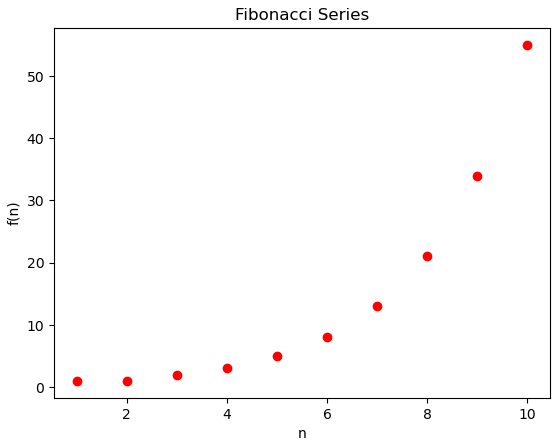
\includegraphics[width=0.5\textwidth]{./chapters/ch-python/figures/fib_exp.png}
\caption{Plot Fibonacci series as scatter plot.}
\label{fig:fib_exp}
\end{figure}

The presentation of the plot can be customized. For example, use \verb|plt.xlim(x1, x2)|, \verb|plt.ylim(y1, y2)| to change the axis limitations, etc. It is possible to change curve color, size, style, and marker size, style, etc.

\subsection{Seaborn}

Seaborn is another visualization library built on top of the Matplotlib library. It tries to standardize the plots with a simple function call. It scarifies some flexibility that Matplotlib offers, but makes plotting easier.

An example of using Seaborn to plot a histogram is given below. The result is given in Fig. \ref{fig:normhistexp}.
\begin{lstlisting}[language=Python]
import numpy as np
import pandas as pd
import matplotlib.pyplot as plt
import seaborn as sns

x = np.random.randn(1000)
plt.figure()
sns.histplot(x, color="red")
plt.title("Histogram Example")
plt.xlabel("x")
plt.ylabel("Count")
\end{lstlisting}

\begin{figure}[htbp]
	\centering
	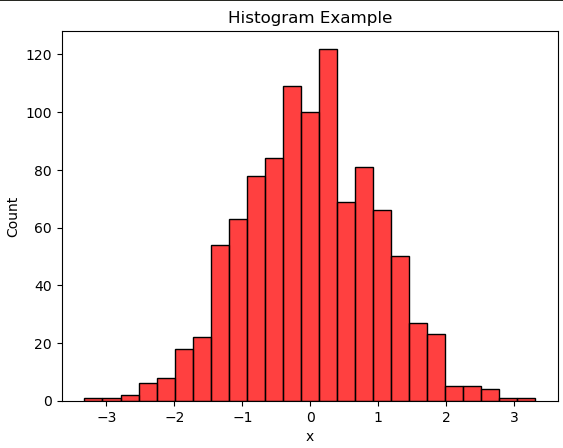
\includegraphics[width=0.5\textwidth]{./chapters/ch-python/figures/normhistexp.png}
	\caption{Histogram plot using Seaborn.}
	\label{fig:normhistexp}
\end{figure}

An example of using Seaborn to plot a count plot for discrete values (usually category values) is given below. Notice that the attribute whose values are put into categories is assigned to $x$ of \verb|seaborn.countplot()|. The result is given in Fig. \ref{fig:countplot}.
\begin{lstlisting}[language=Python]
import numpy as np
import pandas as pd
import matplotlib.pyplot as plt
import seaborn as sns

response = ["yes", "no", "no", "yes", "yes", "yes", "yes", "yes", "yes", "no", "yes", "yes", "NA", "NA"]
plt.figure()
sns.countplot(x=response, color="blue")
plt.title("Count Plot Example")
plt.xlabel("response")
plt.ylabel("Count")
\end{lstlisting}

\begin{figure}[htbp]
	\centering
	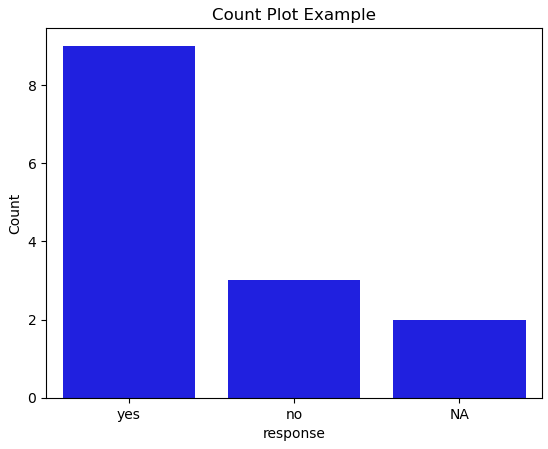
\includegraphics[width=0.5\textwidth]{./chapters/ch-python/figures/countplotexp.png}
	\caption{Count plot using Seaborn.}
	\label{fig:countplot}
\end{figure}

Bot plot gives the maximum, minimum, and interquartile range (IQR) of the data. In the box plot, the data is split into 4 parts, namely $x<Q_1$ ($0\%-25\%$), $Q_1<x<Q_2$ ($25\%-50\%$), $Q_2<x<Q_3$ ($50\%-75\%$), and $Q_3<x$ ($75\%-100\%$). The IQR gives the range between $Q_1$ and $Q_3$, i.e., the half in the middle $25\%-75\%$. An example is given below. The result is given in Fig. \ref{fig:boxplot}.
\begin{lstlisting}[language=Python]
import numpy as np
import pandas as pd
import matplotlib.pyplot as plt
import seaborn as sns

x = np.random.randn(1000)
plt.figure()
sns.boxplot(x, color="blue")
plt.title("Box Plot Example")
plt.xlabel("Input")
plt.ylabel("Value")
\end{lstlisting}

\begin{figure}[htbp]
	\centering
	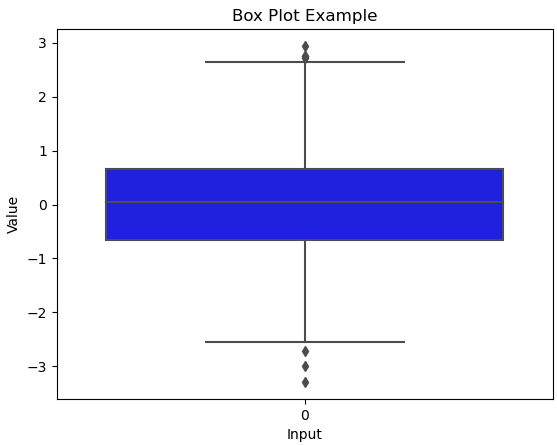
\includegraphics[width=0.5\textwidth]{./chapters/ch-python/figures/boxplotexp.png}
	\caption{Box plot using Seaborn. The box gives IQR. The bars below and above the box give $Q_1-1.5\times\textup{IQR}$ and $Q_3+1.5\times\textup{IQR}$, respectively. The dots are outliers.}
	\label{fig:boxplot}
\end{figure}

There are many more plot functions in Seaborn. For example, scatter plot \verb|seaborn.scatterplot()| works similar with Matplotlib as shown by Fig. \ref{fig:fib_exp}. The marker size and color can be adjusted to reflect different parameters, just like in R language. Pairplot \verb|seaborn.pairplot()| generates a matrix of plots to demonstrate associations of columns in a data frame.

\section{Pandas} \label{sec:pandas}

Many Python packages provide functions to handle structured data such as tables, series, and data frames. Among all these packages, \verb|pandas| is the all-time star that is very widely used by developers and data scientists. With \verb|pandas|, Python gains the ability to easily, flexibly and efficiently deal with data frames. The \verb|pandas| package is introduced in this section.

A large portion of this chapter, including codes and examples, are from online resources such as \textit{Data Analysis by Pandas and Python} on Udemy. My special thanks go to them.

The data frames used in the examples of this chapter may come from different public data resources. It is worth mentioning \textit{kaggle.com}, a place where tens of thousands of data sets, code examples, and notebooks are collected and shared. Some data frames used in the examples come from Kaggle.

Two Python packages, \verb|numpy| and \verb|pandas|, are almost certainly used in all the examples to be presented in this chapter. Import these packages as follows.
\begin{lstlisting}
	import numpy as np
	import pandas as pd
\end{lstlisting}
Unless otherwise mentioned, these packages are always assumed imported in this chapter. To display the packages version, use something like
\begin{lstlisting}
	print("Numpy version: {}.".format(np.__version__))
	print("Pandas version: {}".format(pd.__version__))
\end{lstlisting}

\subsection{Data Importing}

Pandas provide variety of ways to import data from different resources, including plain texts, CSV files, databases, etc. One of the most commonly seen data sources is CSV files. Importing data from CSV files is introduced here.

Pandas provide \verb|.read_csv()| function to import data from CSV files. Its basic usage is introduced below.
\begin{lstlisting}[language=python]
	best_selling_games_df = pd.read_csv("best-selling-video-games.csv")
	best_selling_games_df
\end{lstlisting}
which reads all the information in the CSV table into a data frame as shown by Fig. \ref{fig:dfexp}.
\begin{figure}[htbp]
	\centering
	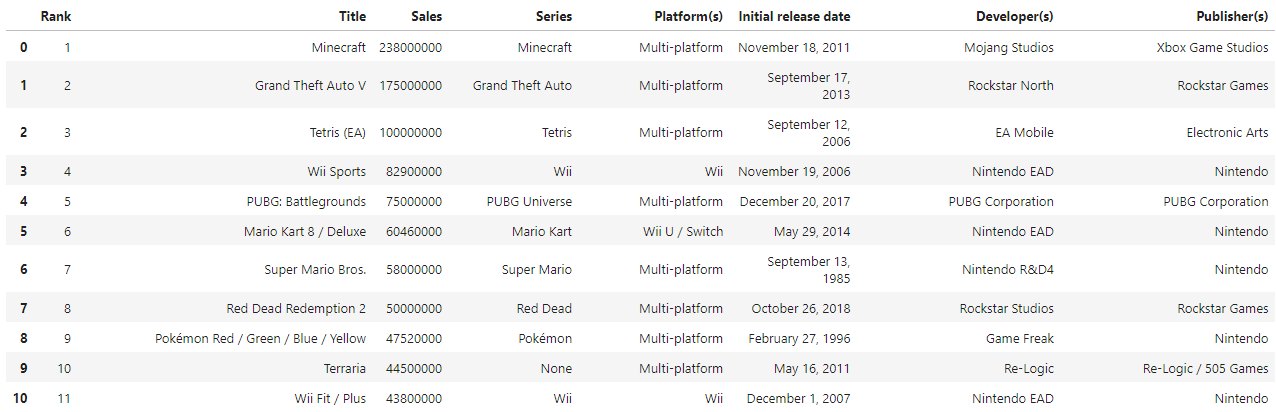
\includegraphics[width=\textwidth]{./chapters/ch-python/figures/df_example.png}
	\caption{The simplest data frame importing using pandas.}
	\label{fig:dfexp}
\end{figure}
It is possible to import only selected columns as follows.
\begin{lstlisting}[language=python]
	best_selling_games_df = pd.read_csv("best-selling-video-games.csv", usecols = ["Title", "Sales", "Publisher(s)"])
	best_selling_games_df
\end{lstlisting}

When no index column is specified, pandas will add an additional auto-incremental column and use it as the index column, as shown in Fig. \ref{fig:dfexp} by the most-left column. When a column index is specified, pandas will use that column as index column. An example is given below. The result is shown in Fig. \ref{fig:dfex2}.
\begin{lstlisting}[language=python]
	best_selling_games_df = pd.read_csv("best-selling-video-games.csv", index_col = "Title", usecols = ["Title", "Sales", "Publisher(s)"])
	best_selling_games_df
\end{lstlisting}
\begin{figure}[htbp]
	\centering
	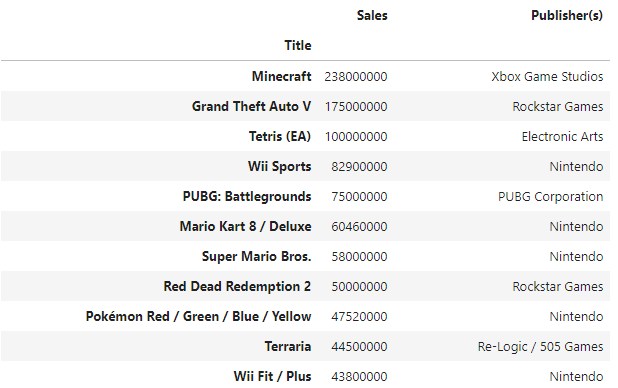
\includegraphics[width=0.5\textwidth]{./chapters/ch-python/figures/df_example2.png}
	\caption{Specifying index column and reading only selected columns using pandas.}
	\label{fig:dfex2}
\end{figure}

It is possible to read the full-size data frame into pandas first, then subsequently select only a few (or event only one) columns to form a new sub data frame. It is possible to take only one column from the data frame, and convert it into a series. Notice that a single-column data frame is different from a series from data type perspective. Examples are given below.
\begin{lstlisting}
	# form sub data frame
	best_selling_games_df = pd.read_csv("best-selling-video-games.csv")
	sub_games_df = best_selling_games_df[["Title", "Sales", "Publisher(s)"]]
	sub_games_df
	# form single-column sub data frame
	sub_games_df = best_selling_games_df[["Title"]]
	sub_games_df
	# convert single-column data frame to series
	best_selling_games_titles = sub_games_df.squeeze('columns')
	best_selling_games_titles
	# get series from data frame directly
	best_selling_games_df = pd.read_csv("best-selling-video-games.csv")
	best_selling_games_titles = best_selling_games_df["Title"]
	best_selling_games_titles
\end{lstlisting}

It is worth mentioning that when generating series from data frames, the index column of the data frame is inherited by the series. This introduces an important feature of pandas series: unlike Python array where it is just single-stream sequence of data, pandas series has a separate measure of index for each element in the series, essentially making it multi-stream of data. More are introduced in later sections.

\subsection{Series and Data Frame}


\chapter{Kubernetes}

Kubernetes is introduced cross sections. This section focuses on a brief introduction to Kubernetes, its basic schematic architecture, and how it can be installed on a local machine.

\section{Basic Kubernetes}

\textit{Kubernetes}, also known as \textit{k8s}, is an open-source container orchestration system originally developed by Google. It automates the deployment, scaling, and management of containerized applications. While Kubernetes is more flexible than Portainer, it's also more complex and has a steeper learning curve.

Note that running Kubernetes on a local server can differ significantly from running it on a cloud platform such as AWS or Google Cloud, which offer managed Kubernetes services with additional features and simplified management. These platforms, AWS with its Elastic Kubernetes Service (EKS) and Google Cloud with Google Kubernetes Engine (GKE), have developed their own tools and interfaces for interacting with Kubernetes. So, while learning Kubernetes can be beneficial, one might not need to learn all the low-level details if he is running Kubernetes using one of the above management tools instead of DIY everything.

This notebook focuses introducing running Kubernetes on a local server in a DIY manner. In this scenario, the following common practice is adopted: \textit{kubectl} is used as the user interface to Kubernetes and \textit{minikube} the software to manage the host machine. Minikube is an open-source software developed by the Kubernetes community to run a single-node Kubernetes cluster on a local machine, which is suitable for developers to learn and test different things in development environment.

Notice that in the past days, docker is the default container engine built-in to Kubernetes, and Kubernetes uses a special program ``dockershim'' that talks to docker engine. As of now, docker support is deprecated in Kubernetes and dockershim is removed from the installation.

\subsection{Infrastructure}

Figure \ref{ch:vac:fig:kubernetescluster} demonstrates what key components Kubernetes has inside its cluster.
\begin{figure}
	\centering
	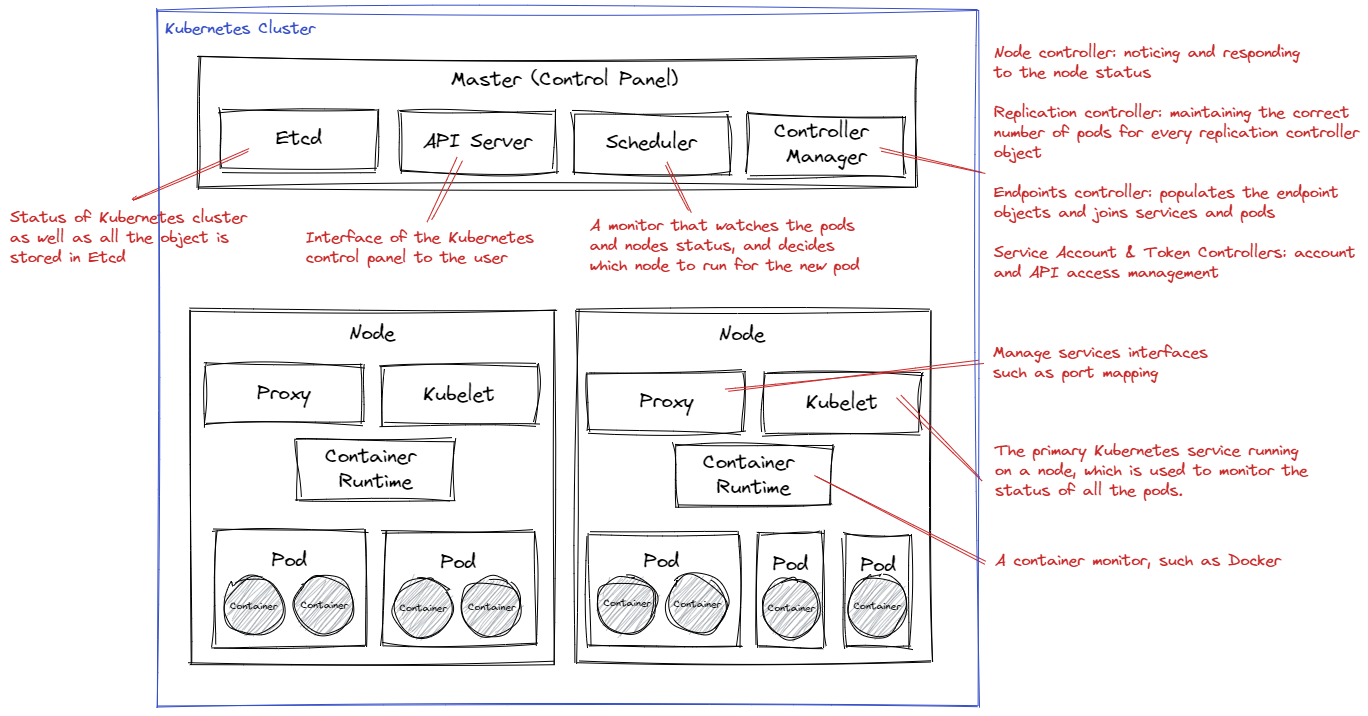
\includegraphics[width=350pt]{chapters/ch-virtualization-and-containerization/figures/kubernetescluster.png}
	\caption{Kubernetes cluster and its key components.} \label{ch:vac:fig:kubernetescluster}
\end{figure}
As shown in Fig. \ref{ch:vac:fig:kubernetescluster}, Kubernetes manages containers in a centralized ``master-worker'' mode, where the master plays as the control panel, API gateway (with static IP address) and load balancer to interact with a user, and the worker nodes (also known as nodes, for short) actually process the data. Each node can host multiple pods, inside each pod is a container or a group of containers that work closely together. Notice that in Kubernetes, containers never run directly in a node. They are always grouped into pods. A pod should be the minimal unit or group of container(s) that can deliver a basic function.

In practice, the master and nodes can run on cross servers or VMs. Kubernetes packages need to be installed on each and every server or VM for the system to work properly. Kubernetes provides variety of tools to distribute the loads to different servers or VMs, or to add redundancy to the system for high availability.

\subsection{Installation}

The installation guidance of Kubernetes can be found at its official website \textit{kubernetes.io}. Notice that different OS adopts different ways of installing and using Kubernetes. The installation procedures introduced in this section applies to Linux OS only. For Windows users, Kubernetes can be installed from Docker desktop. For macOS users, other tools are used to install the tools to be introduced below.

As introduced earlier, \textit{kubectl} is used to interact with Kubernetes. In addition, since we are in development environment, we will also install \textit{minikube} which is used to setup a small Kubernetes cluster in the local machine. They can be installed separately. See following links for more details.
\begin{lstlisting}
	https://kubernetes.io/docs/tasks/tools/install-kubectl-linux/
	https://minikube.sigs.k8s.io/docs/start/
\end{lstlisting}
When running \textit{minikube} for the first time, it would try to install \textit{kubectl} as a built-in. Start \textit{minikube} using \verb|minikube start|, which will start a VM using Vertual Box, and setup a single Kubernetes node in the VM.

If \textit{kubectl} and \textit{minikube} are installed separately, run the following command to verify the successful installation of both software.
\begin{lstlisting}
	$ kubectl cluster-info
	Kubernetes control plane is running at https://192.168.49.2:8443
	CoreDNS is running at https://192.168.49.2:8443/api/v1/namespaces/kube-system/services/kube-dns:dns/proxy
\end{lstlisting}

If \textit{minikube} is installed, and \textit{kubectl} is considered as a built-in installation to \textit{minikube}, use the following command
\begin{lstlisting}
	$ minikube kubectl cluster-info
	Kubernetes control plane is running at https://192.168.49.2:8443
	CoreDNS is running at https://192.168.49.2:8443/api/v1/namespaces/kube-system/services/kube-dns:dns/proxy
\end{lstlisting}
in which case \verb|alias kubectl="minikube kubectl --"| may make things easier.

It is indeed possible to run Docker and Kubernetes directly on a host machine if that machine is running a Linux OS. However, this is typically not recommended for reasons pertaining to access control, security, and isolation. It is generally better practice, particularly in a development environment, to deploy your Kubernetes cluster within a virtual machine.

The \verb|kubectl| command is a command-line interface (CLI) for interacting with Kubernetes clusters. Its behavior is governed by a configuration file, typically located at \verb|~/.kube/config|, which determines which Kubernetes cluster \verb|kubectl| communicates with. This could be a cluster running on the host machine, or a cluster running in a VM managed by tools like Minikube. It's worth noting that, for better isolation and control, it is recommended to deploy the Kubernetes cluster in a VM, instead of directly on the host machine.

\subsection{Kubernetes Configuration Files}

Managing containers via container orchestration such as Kubernetes is different from doing so using container engines such as docker engine. Unlike docker engine where we started from building an image from a dockerfile, Kubernetes requires that all images to be used are already available. Instead of having one configuration file where each entry in that file corresponds with a container, when using Kubernetes, multiple configuration files are required, each file corresponding with an object to be created. Notice that an object is not necessarily a container. It can be a pod, a replica controller, a service, or any other ``thing'' in the Kubernetes framework. There are more involving manual setups of networking when using Kubernetes as well. Details are introduced in the remaining of this section.

The following two configuration files are given as examples \cite{stephen2023docker} to demonstrate how these files look like. This example comes from Udemy course \textit{Docker and Kubernetes: The Complete Guide} by Stephen Grinder. They are both written in YAML. Configuration file to setup a pod:
\begin{lstlisting}
	apiVersion: v1
	kind: Pod
	metadata:
	name: client-pod
	labels:
	component: web
	spec:
	containers:
	- name: client
	image: <image-name>
	ports:
	- containerPort: 3000
\end{lstlisting}
Configuration file to setup the networking service:
\begin{lstlisting}
	apiVersion: v1
	kind: Service
	metadata:
	name: client-node-port
	spec:
	type: NodePort
	ports:
	- port: 3050
	targetPort: 3000
	nodePort: 31515
	selector:
	component: web
\end{lstlisting}

Commonly used Kubernetes object types are summarized in Table \ref{ch:vac:tab:objtype}.
\begin{table}[htbp]
	\centering
	\caption{Commonly used Kubernetes object types.} \label{ch:vac:tab:objtype}
	\begin{tabularx}{\textwidth}{lX}
		\hline
		Object Type & Description \\
		\hline
		Pod & The smallest and most basic unit in the Kubernetes object model. It represents a single instance of a process running on the cluster. \\ \hdashline
		Deployment & Manages the deployment and scaling of a set of identical pods, ensuring the desired number of replicas are running and providing rolling updates for seamless application upgrades. \\ \hdashline
		Service & Enables network access to a set of pods using a stable IP address and DNS name. It provides load balancing across multiple pod replicas and allows external traffic to be directed to the appropriate pods. \\ \hdashline
		ConfigMap & Stores configuration data in key-value pairs, which can be consumed by pods as environment variables, command-line arguments, or mounted as files. \\ \hdashline
		Secret & Similar to a ConfigMap, but specifically designed to store sensitive data, such as passwords, API keys, and TLS certificates. Secrets are encrypted at rest and can be mounted into pods as files or exposed as environment variables. \\ \hdashline
		PersistentVolume & Provides a way to provision and manage persistent storage resources in a cluster. It decouples the storage from the underlying infrastructure and allows data to persist beyond the lifecycle of individual pods. \\ \hdashline
		PersistentVolumeClaim & Requests a specific amount of storage from a PersistentVolume. It acts as a request for a specific storage resource and provides an abstraction layer for managing persistent storage in a cluster. \\ \hdashline
		Ingress & Manages external access to services within a cluster. It acts as a reverse proxy and exposes HTTP and HTTPS routes to route traffic to the appropriate services based on hostnames, paths, or other rules. \\
		\hline
	\end{tabularx}
\end{table}
Some highlights of the above configuration files are as follows.
\begin{itemize}
	\item \verb|apiVersion| plays as the prefix that decides what configuration types are supported. For example, under the scope of \verb|v1|, \verb|Pod|, \verb|Service|, \verb|configMap|, \verb|Namespace|, etc., are supported. In a different \verb|apps/v1|, a different set of configuration types \verb|ControllerRevision|, \verb|StatefulSet|, etc., are supported. It's important to choose the correct apiVersion for the Kubernetes API version you are working with to ensure the compatibility and availability of the desired configuration options.
	\item \verb|kind| This indicates the type of the object that the configuration file describes. For example, \verb|Pod| represents a pod that is used to host containers, and \verb|Service| the primary object type that defines networking, with subtypes \verb|NodePort| (see example above), \verb|ClusterIP|, \verb|LoadBalancer| and \verb|Ingress|.
	\item \verb|metadata| indicates the name and labels of the object. For example, \verb|component: web| is defined as a label of the pod. This information is passed to the networking service under \verb|selector|, so that the networking service knows which object it should link to.
	\item \verb|port|, \verb|targetPort| and \verb|nodePort| are used to specify ports used in the service. The \verb|targetPort| indicates which port in the pod should be exposed to the service, and it is consistent with \verb|containerPort| defined in the pod. Assume that there is another pod in the node who needs to talk to this pod via the service. The other pod's port that communicates with the service is fed into \verb|port|. Finally, \verb|nodePort| is the port with value between 30000 and 32767 that is exposed from the service to outside the node. If \verb|nodePort| is not assigned, a random number within the range will be assigned. This is shown in Fig. \ref{ch:vac:fig:nodeport}.
\end{itemize}
Notice that Kubernetes networking using \verb|kind: Service| is more complicated than shown in the above example. More details of it is given later in a dedicated Section \ref{ch:vac:subsec:k8snetworking}.

\begin{figure}
	\centering
	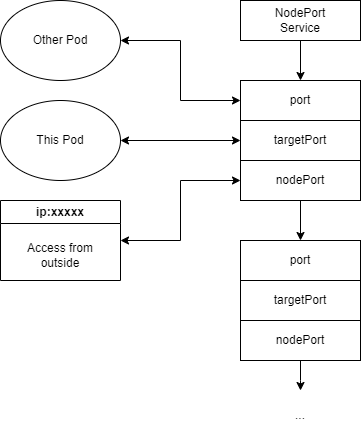
\includegraphics[width=200pt]{chapters/ch-virtualization-and-containerization/figures/nodeport.png}
	\caption{The NodePort networking service.} \label{ch:vac:fig:nodeport}
\end{figure}

\subsection{Cluster Deployment}

With the image and the configuration files ready, the next step is to deploy the nodes, pods, and containers. \textit{kubectl} command line interface is used to instruct Kubernetes to deploy the objects as follows.
\begin{lstlisting}
	$ kubectl apply -f <configuration file>
\end{lstlisting}
This essentially asks the master node in the Kubernetes cluster to start taking actions according to the configuration files, such as to inform the nodes to start creating pods and containers. The master node also keeps monitoring the status of each work node, to make sure that everything is running as planned. If there is a container failure, etc., the master node will guide the associated note to restart the container.

It is worth mentioning here that by default Kubernetes uses declarative deployment instead of imperative deployment, meaning that the developer does not need to specifically tell Kubernetes what to do in each step. The developer only tells the overall objectives, and Kubernetes master node will try to figure out the steps to realize that goal. It is possible to enforce Kubernetes master node to practice specific details via configuration files, but it is almost always recommended to use the default declarative approach with Kubernetes.

To retrieve information, such as the status, of a group of objects, use
\begin{lstlisting}
	$ kubectl get <object type>
\end{lstlisting}
where \verb|<object type>| can be \verb|pods|, \verb|services|, etc. For more details of a specific object, use
\begin{lstlisting}
	$ kubectl describe <object type> <object name>
\end{lstlisting}
for example, to check the containers running in a pod. If \verb|<object name>| is neglected, Kubernetes returns detailed information of all objects of the given object type. For a running object, use
\begin{lstlisting}
	$ kubectl logs <object name>
\end{lstlisting}
to check the log file of that object.

With the above been done, open a browser and use \verb|<ip>:<port>| to access the application running in the container, where \verb|<ip>| is the IP address of the VM (not \verb|localhost|) that \textit{minikube} created, and \verb|<port>| the port configured in NodePort service under \verb|nodePort|. The IP address can be found by running \verb|minikube ip|.

To apply a group of configuration files all together, provide the directory name of all the configuration files to Kubernetes instead of feeding each configuration file one at a time.
\begin{lstlisting}
	$ kubectl apply -f <directory>
\end{lstlisting}
When directory is given instead of a file, Kubernetes will try to apply all the configuration files in that directory.

It is possible to consolidate the configuration files of objects into one conjunctive configuration file. To do that, use \verb|---| to split the configurations for each object in the conjunctive configuration file as follows. It is of personal preference whether to use conjunctive configuration files or separate configuration files for all objects.
\begin{lstlisting}
	<configurations-for-object-1>
	---
	<configurations-for-object-2>
	---
	<...>
\end{lstlisting}

\subsection{Cluster Update} \label{ch:vac:subsec:updatek8s}

Without container orchestration such as Kubernetes, one of the most challenging tasks is to update the container for a different configuration, for example, changing the underlying image. With the help of Kubernetes declarative approach, it is possible update the cluster simply by revising the configuration files, and pass them to Kubernetes as if the cluster is to be deployed for the first time. Kubernetes automatically checks the names and kinds of the revised configuration files, comparing them with existing running objects, and update them if necessary.

Check the status of the pods using \verb|kubectl get pods|. After updating, the pods are often restarted, hence it is expected to see increment in the ``RESTARTS'' tag. To double confirm that updates have been made, use \verb|kubectl describe| to check the details of the relevant objects.

However, there is a limitation to the updating of the Kubernetes deployment. For an existing object, only certain fields in the configuration files can be changed. For example, for a pod that runs containers, the image can be changed, but the container port cannot. Sometimes there can be a walk around. For example, in the case of changing container port of pods, consider using a new object type \verb|Deployment| instead of \verb|Pod|, which allows more flexible updating. The \verb|Deployment| in its backend is consist of one or more monitored and managed identical pods.

To revert \verb|kubectl apply|, i.e., to remove a configuration file, use
\begin{lstlisting}
	$ kubectl delete -f <configuration file>
\end{lstlisting}
Kubernetes treats the above delete command as a specific type of update to the cluster, and will action accordingly.

\section{Advanced Kubernetes}

This section introduces advanced commonly used Kubernetes objects, tools and techniques.

\subsection{Kubernetes Object: Deployment} \label{ch:vac:subsec:deployment}

As introduced in Section \ref{ch:vac:subsec:updatek8s}, updating pods has some limitations. It is practically more convenient to setup pods using ``Deployment'' object instead of ``pod''. The Deployment object servers as an additional layer of Kubernetes infrastructure that manages identical pods. More details of Deployment object is introduced in this section.

As an example, here is a configuration file from Kubernetes manual that deploys a Deployment object.
\begin{lstlisting}
	apiVersion: apps/v1
	kind: Deployment
	metadata:
	name: nginx-deployment
	labels:
	app: nginx
	spec:
	replicas: 3
	selector:
	matchLabels:
	app: nginx
	template:
	metadata:
	labels:
	app: nginx
	spec:
	containers:
	- name: nginx
	image: nginx
	ports:
	- containerPort: 80
\end{lstlisting}
Some highlights are as follows.
\begin{itemize}
	\item \verb|replicas| gives the expected number of pods that the Deployment object manages.
	\item \verb|matchLabels| specifies the pods with which label are to be managed by the Deployment object. In this example, the label is \verb|app: nginx|. When populating pods, the pods would have the same label, as the same label is assigned under \verb|template|, \verb|metadata|, \verb|labels|.
	\item \verb|template| specifies the template that is used to create the pods.
\end{itemize}

When a new version of an image becomes available, we may want to update the containers accordingly. Re-apply the same configuration file would not help, as Kubernetes would reject apply request if no change is detected in the configuration file. It would not check whether the image is in its latest version. Kubernetes uses the following imperial command to update images as a walk around, and the developer needs to run this command manually.
\begin{lstlisting}
	$ kubectl set image deployment/<Deployment name> <container name>=<image name>
\end{lstlisting}
For example,
\begin{lstlisting}
	$ kubectl set image deployment/nginx-deployment nginx=nginx:1.25.1
\end{lstlisting}

\subsection{Kubernetes Object: Service} \label{ch:vac:subsec:k8snetworking}

There are 4 service types defined in Kubernetes. So far ``NodePort'' service type has been introduced in earlier examples. More types are introduced here.

A summary of different service types are given below.
\begin{itemize}
	\item ClusterIP: Exposes the service object on a cluster-internal IP. Objects in the cluster can access to the object that a ClusterIP is pointing at.
	\item NodePort: Assigns a static port with the cluster IP, and exposes the Service object to the internet. This is used mostly used in development environment, not in production environment.
	\item LoadBalancer: Exposes the service object externally using an external load balancer. Kubernetes does not provide built-in load balancer.
	\item ExternalName: Maps the service object to the contents of the \verb|externalName| field, such as a host name. This is related to cluster DNS server.
\end{itemize}

\vspace{0.1in}
\noindent \textbf{ClusterIP}
\vspace{0.1in}

A ClusterIP configuration file may look like the following.
\begin{lstlisting}
	apiVersion: v1
	kind: Service
	metadata:
	name: client-cluster-ip-service
	spec:
	type: ClusterIP
	selector:
	<target tag>
	ports:
	- port: <port for internal comm>
	targetPort: <port for internal comm>
\end{lstlisting}
where the first \verb|port for internal comm| is the port in the ClusterIP service object that opens to other objects in the cluster, and the second the port the target object opens to the ClusterIP service object. They can be set differently, but usually they are just set to the same value.

\vspace{0.1in}
\noindent \textbf{NodePort}
\vspace{0.1in}

NodePort has already been introduced earlier. It exposes the object to the internet with a static port, and it is used more in a development environment than a production environment.

\vspace{0.1in}
\noindent \textbf{LoadBalancer}
\vspace{0.1in}

LoadBalancer is a legacy way of getting network traffic into the pods. It is essentially an interface or a tool to bridge an Kubernetes Deployment with an external load balancer. It will try to automatically configure the external load balancer using the configuration provided by the developer, while compromising the external load balancer rule.

\vspace{0.1in}
\noindent \textbf{Ingress}
\vspace{0.1in}

Ingress is a more commonly used Service type than LoadBalancer to get traffic into the Kubernetes containers. There are different types of Ingress, for example, Nginx Ingress by \textit{github.com/kubernetes/ingress-nginx}. An demonstrative example of ingress service realization is given in Fig. \ref{ch:vac:fig:ingress_service}. In this implementation framework, the configuration file (mainly a set of routing rules) of the object is used to define an ``Ingress Controller'' which manages the runtime that controls inbound traffic. In some applications such as \textit{kubernetes/ingress-nginx}, the ingress controller and the runtime are integrated together.

\begin{figure}
	\centering
	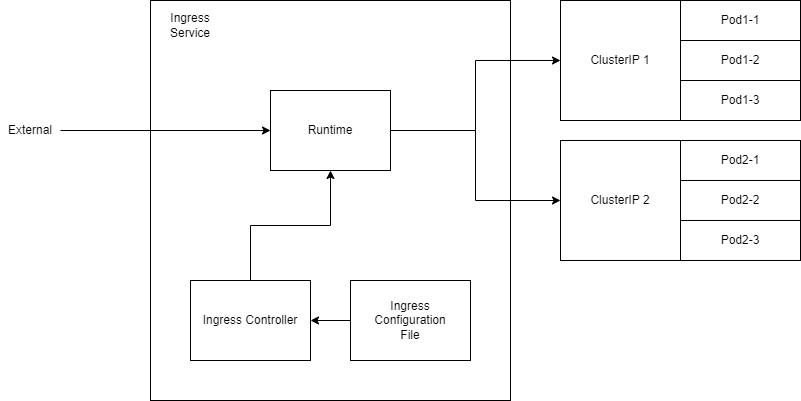
\includegraphics[width=350pt]{chapters/ch-virtualization-and-containerization/figures/ingress_service.png}
	\caption{An example of ingress service framework.} \label{ch:vac:fig:ingress_service}
\end{figure}

The ingress configuration differs depending on the ingress service type and the platform. Details are not given here.

\subsection{Kubernetes Object: Persistent Volume Claim, Persistent Volume, and Volume} \label{ch:vac:subsec:k8svolume}

Docker engine uses volumes to maintain persistent data and share data among containers. Details have been introduced in Section \ref{ch:vac:subsec:dockervolume}. Kubernetes volume framework is similar in the sense that it makes sure that the data is saved and managed by the host machine, so that when the pods or containers are shutdown or restarted, the data can be restored safely.

Do notice that when comes to data sharing using volume, it is dangerous to have multiple containers or the host machine accessing the same files simultaneously, without knowing the existence of each other. Usually additional steps need to be setup to ensure data consistency.

It is worth emphasizing the differences of ``volume'' technology in containerization and Kubernetes volume-related objects: Persistent Volume Claim (PVC). Persistent Volume (PV), and Volume. As a matter of fact, Kubernetes Volume object is usually not what we want. Kubernetes Volume creates the volume tied to a pod, not to the host machine. It survives container failure in the pod, but not pod failure. In summary:
\begin{itemize}
	\item Kubernetes Volume: A volume tied to the pod. It survives container failure inside the pod, but not pod failure.
	\item Kubernetes PV: A volume tied to the host machine. It survives pod failure. It can be provisioned either automatically by a StorageClass, or manually by the developer and administrator.
	\item Kubernetes PVC: It is essentially a request sent from a pod or a container, asking for specific amount of storage from a PV. Kubernetes will find that amount of PV from either existing provisioned static PV, or dynamically provision new ones for the pod or container.
\end{itemize}
Notice that it is not necessary to claim PV in order to use PVC, as PVC can provision PV dynamically. There is a one-to-one relationship between the provisioned PV and the PVC. If there are multiple pods, each requiring a dedicated PV, then multiple PVCs must be used. The developer can either create those PVCs manually, or use a Volume Claim Template to claim them if they are similar.

An example of claiming Kubernetes PV and PVC is given below. In the remaining part of this section, we will be mostly using PVC instead of PV.
\begin{lstlisting}
	# persistent-volume.yaml
	
	apiVersion: v1
	kind: PersistentVolume
	metadata:
	name: my-pv
	spec:
	storageClassName: standard
	capacity:
	storage: 10Gi
	accessModes:
	- ReadWriteOnce
	hostPath:
	path: /data/my-pv
	---
	# persistent-volume-claim.yaml
	
	apiVersion: v1
	kind: PersistentVolumeClaim
	metadata:
	name: my-pvc
	spec:
	storageClassName: standard
	accessModes:
	- ReadWriteOnce
	resources:
	requests:
	storage: 5Gi
\end{lstlisting}
To check the PV objects, use \verb|$ kubectl get pv| and \verb|$ kubectl get pvc|.

To add the above Kubernetes PVC to a Kubernetes Deployment, add volumes information to the specs as given in the following example.
\begin{lstlisting}
	apiVersion: apps/v1
	kind: Deployment
	metadata:
	name: my-app-deployment
	spec:
	replicas: 1
	selector:
	matchLabels:
	app: my-app
	template:
	metadata:
	labels:
	app: my-app
	spec:
	containers:
	- name: my-app-container
	image: my-app-image
	ports:
	- containerPort: 8080
	volumeMounts:
	- name: data-volume
	mountPath: /data
	subPath: data-from-container
	volumes:
	- name: data-volume
	persistentVolumeClaim:
	claimName: my-pvc
\end{lstlisting}
where \verb|volumes| defines which Kubernetes PVC is used, and \verb|volumeMounts| tells how it is mounted in the container. The \verb|mountPath| is the path in the container whose data is mounted by the volume. If a \verb|subPath| is given, a sub-folder of its specified name will be created in the host machine in the volume to contain the data.

There are different types of access modes: 
\begin{itemize}
	\item \verb|ReadWriteOnce|: Allow one node to read and write at a time.
	\item \verb|ReadOnlyMany|: Allow many nodes to read at a time.
	\item \verb|ReadWriteMany|: Allow many nodes to read and write at a time.
\end{itemize}

The developer can specify the place for Kubernetes PVs. This is usually the hard drive on a local server, a virtual storage space in the VM. Use the following command to check Kubernetes possible choice of storage.
\begin{lstlisting}
	$ kubectl get storageclass
\end{lstlisting}
and 
\begin{lstlisting}
	$ kubectl describe storageclass
\end{lstlisting}
When deploying Kubernetes on the Cloud, the developer needs to do additional configurations as there would be many storage options. Usually, each Cloud provider will have its own default storage space for Kubernetes, such as AWS Elastic Block Store for AWS.

\subsection{Kubernetes Object: Secrets} \label{ch:vac:subsec:k8ssecrets}

Kubernetes Secrets object is used store confidential information, such as the database password, API key, etc. It is often a piece of information that is necessary for the containers, but the developer does not want to present as plain text in the configuration file.

Secrets are not created from configuration files, which is the recommended way of creating other Kubernetes objects. Instead, it is created from one-time imperative command, inside which the confidential information needs to be told to Kubernetes. Use the following command to create a Secret object.
\begin{lstlisting}
	$ kubectl create secret <type-of-secret> <secret-name> --from-literal <key>=<value>
\end{lstlisting}
There are 3 types of Secrets: \verb|generic|, \verb|docker-registry| and \verb|tls|.

\subsection{Kubernetes Environment Variables}

Kubernetes environment variables are used to pass or share information among Deployments. Depending on the features of the information, such as whether it is a constant global configuration or a dynamic value, whether it is plain text or confidential encoding, etc., it might be handled differently.

To define constant environment variables in containers, simply specify them in the Deployment configuration file as given in the example below.

\begin{lstlisting}
	apiVersion: apps/v1
	kind: Deployment
	metadata:
	name: my-app-deployment
	spec:
	replicas: 1
	selector:
	matchLabels:
	app: my-app
	template:
	metadata:
	labels:
	app: my-app
	spec:
	containers:
	- name: my-app-container
	image: my-app-image
	ports:
	- containerPort: 8080
	volumeMounts:
	- name: data-volume
	mountPath: /data
	subPath: data-from-container
	env:
	- name: <name1>
	value: <value1>
	- name: <name2>
	value: <value2>
	- name: <name3>
	valueFrom:
	secretKeyRef:
	name: <secret-name>
	key: <key>
	volumes:
	- name: data-volume
	persistentVolumeClaim:
	claimName: my-pvc
\end{lstlisting}
where a new tag \verb|env| is defined under template, specifications, containers. Under the \verb|env| tag, a list is defined containing names and values of the environment variables. The value must be a string, not a numerical number.

\section{Container Deployment in Production Environment}

With the tools and methodologies introduced so far, we are able to deploy containers in development environment. This is good enough for testing purpose or for small individual projects. However, when comes to enterprise tier projects or collaborative projects, there is often a CI/CD pipeline that standardize the integration and delivery of the containers in production environment. Container orchestrations such as Kubernetes is often a must have.

This section briefly introduces the steps to develop and deploy containers in production environment with Kubernetes. Figure \ref{ch:vac:fig:prodenvworkflow} gives an example of overview of what such deployment may look like. Notice that this example is more towards a community project but not an enterprise project.

\begin{figure}
	\centering
	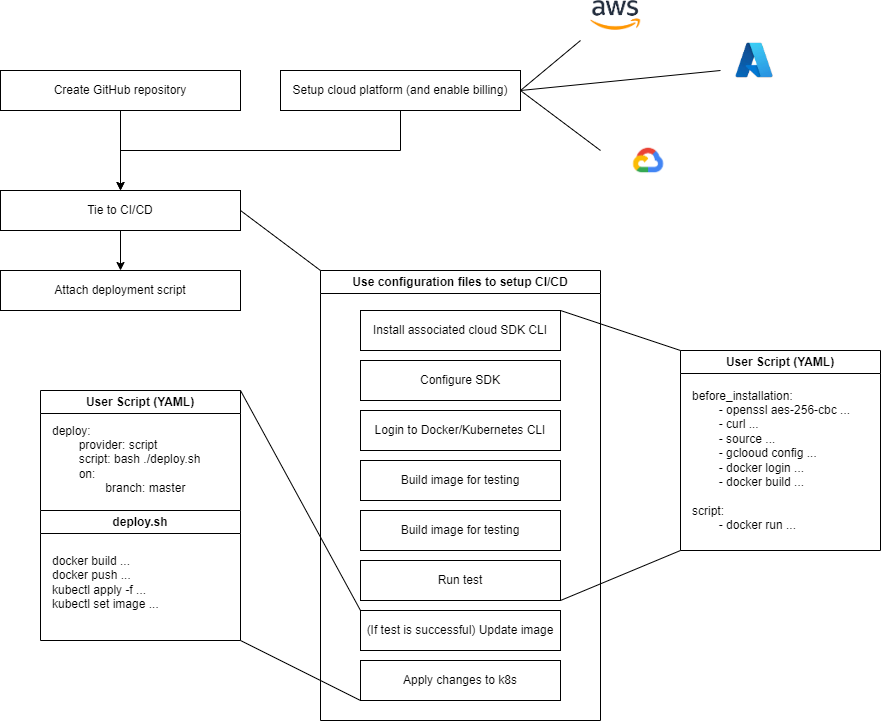
\includegraphics[width=350pt]{chapters/ch-virtualization-and-containerization/figures/prodenvworkflow.png}
	\caption{An example workflow of creating a production environment with Kubernetes.} \label{ch:vac:fig:prodenvworkflow}
\end{figure}

The example used in this section to demonstrate Kubernetes CI/CD on a cloud platform in production environment is taken from \cite{stephen2023docker}. Following \cite{stephen2023docker}, Google Cloud Platform is used as the cloud platform provider.

\subsection{Setup Cloud Account}

Many cloud platforms nowadays have a very good support of Kubernetes. The deployment of containers using Kubernetes can be done via their UIs easily. The developer needs to decide the resources to be used for the deployment. The more nodes and more power machine, the higher the charge. In most cases, the developer does not need to start a VM and install Kubernetes on it by himself. The cloud provider shall have dedicated Kubernetes engine service that would automatically configure the VM per required.

\subsection{Configure CI/CD}

Travis CI is a continuous integration service tool written. It can be deployed on the cloud and linked to a Github repository and a CI/CD platform such as a Kubernetes cluster on Google Cloud Platform.

To run Travis, a machine supporting Ruby programming language is required. For that, a separate container with Ruby installation is deployed to run Travis. Use Github credentials to login to Travis, so that it can link to the Github repositories.

Travis has built-in file encryption function. This function is mainly used to encrypt login credentials and service account credentials (in this example, the service account information to link to Kubernetes clusters on Google Cloud Platform) locally, so that later the unencrypted original credential files can be deleted, and only the encrypted credentials uploaded to the Github repository. When encrypting a file, Travis will also guide the user on how to call the encrypt information in the build script. 

Travis uses configuration files to setup CI/CD pipeline.

\subsection{Deploy Containers}

In the Travis configuration file, \verb|deploy| is used to specify the script to run when the testing is successful. A separate bash script \verb|deploy.sh| is defined for this purpose, inside which is a sequence of commands that builds and publishes images, and configures Kubernetes using \verb|kubectl|.

It is particularly worth mention that in \verb|deploy.sh|, when building and applying the latest version of the docker image, tagging using \verb|<image-name>:latest| alone is not going to work for the same reason explained earlier in Section \ref{ch:vac:subsec:deployment}: when the same configuration with \verb|<image-name>:latest| is applied, the system would simply acknowledge it as ``no change'' and would not actually download the latest version of the image.

The walk around introduced in Section \ref{ch:vac:subsec:deployment} was to use version number in the configuration file and/or as an imperial command as follows.
\begin{lstlisting}
	$ kubectl set image deployment/<Deployment name> <container name>=<image name>:<version>
\end{lstlisting}
so what when the version name changes, Kubernetes would notice the differences and apply the new image. When working with CI/CD using \textit{Git}, this can be further automated. Just use the \verb|$GIT_SHA| as part of the tag as follows.
\begin{lstlisting}
	docker build -t <docker-id>/<image-name>:latest -t <docker-id>/<image-name>:$GIT_SHA -f <dockerfile> <save-directory>
	docker push <docker-id>/<image-name>:latest 
	docker push <docker-id>/<image-name>:$GIT_SHA
\end{lstlisting}
Notice that in addition to \verb|:latest|, \verb|:$GIT_SHA| is used as a secondary tag. When pushing the built image to Docker hub, both \verb|:latest| and \verb|:$GIT_SHA| are pushed (although they have identical content). When setting image, the \verb|$GIT_SHA| is used to identify the image just like the version number.

It is recommended not to remove \verb|:latest| in the building command. This is because if someone wants to pull and test the latest image in his server (without knowing the value of \verb|$GIT_SHA| for the latest commit), he is still able to do so using only the image name.

Notice that \verb|$GIT_SHA| is not a built-in environment variable. The developer needs to set that environmental variable manually in the configuration YAML file as follows. It is possible to replace \verb|$GIT_SHA| with a different name.
\begin{lstlisting}
	env:
	global:
	- GIT_SHA=$(git rev-parse HEAD)
\end{lstlisting}
With the above setup, \verb|$GIT_SHA| can be used in \verb|deploy.sh| as an environmental variable.

\subsection{Manage Secrets}

Notice that when CI/CD tool is tied to the cloud platform provider, service account authentication is required. It is a good habit to NOT to put the authentication information in the CI/CD configuration file as plain text, or to upload the unencrypted file that contains the authentication information to the public workspace. It is possible that some CI/CD tools provide encryption tools that can be used to encrypt the authentication file. In such case, the developer may need to install the required CLI for that CI/CD tool.

In Section \ref{ch:vac:subsec:k8ssecrets}, it has been introduced that Kubernetes uses Secrets object to encrypt secret files. The encrypted secret files can then be safely published online. In the Kubernetes configuration file, an environmental variable can be created to call the secret information.

Many cloud platform providers including Google Cloud Platform provides services to manage secrets.

\subsection{Helm}

To install a software in a Kubernetes pod, the most intuitive way is to commit the installation in the image, and call the image in the Kubernetes configuration file. For commonly used services such as \verb|ingress-nginx|, its installation configuration file is available online as part of the manual. It essentially starts and initializes a branch of Kubernetes objects to enable the service.

Helm is designed as an alternative to manage software installation in Kubernetes clusters. In many occasions, it is more convenient (or even only possible) to use Helm to install a software. More details are given in \textit{github.com/helm/helm}. 

We need to first install Helm from script. Helm installation used to contain two parts, the CLI (referred as Helm client) and the server (referred as Tiller server). We could then use Helm CLI to install other third-party software and tools. 

Access control is important on cloud platforms. In practice, user accounts are used to identify users, and service accounts to identify pods and programs. Associated role bindings are used to manage what resources can be accessed by a user or program. For example, administrative role over the entire account can be used to bind with the administrative user. The same applies to Helm. The Tiller server required some extent of administrative control over the resources in an account. In many occasions, Tiller server was given the administrative permission to access the entire account, which introduced security risks.

As of Helm version 3, a major change was carried out where Tiller server was removed completely. Helm architecture is more secure and simpler today. The concerns related to Tiller's permission in the Kubernetes cluster are no longer relevant. Helm 3 of course requires permissions to use the resources, which is now managed by Kubernetes role-based access control mechanisms.


\part{Linux Security}

% Linux Security

% Security Enhanced Linux

% Firewall

\part{Linux on Cloud}

% General introduction to cloud computing

\chapter{Estimation of Population Statistics} \label{ch:estimation}

The statistics of the population, such as its mean, variance, etc., can be estimated using the samples. For more insights, we can assume a distribution for the population, and consequently using the samples to estimate the 
parameters in the distribution. Commonly seen methods are introduced in this section.

\section{Method of Moments}

The statistics of the samples can in some extent reflect the system. The most intuitive assumption that one may make is that the samples share the same statistical features with the population. The larger size of the sample set, the more likely this statement is true. This statement can be proved correct for some of the statistical properties such as the mean.

\subsection{Mean and Variance}

The sample mean and variance are calculated as follows. Let $X_1, \ldots, X_m$ be the samples. For sampling number $m\geq 2$,
\begin{eqnarray}
	\bar{X} &=& \dfrac{1}{m}\sum_{i=1}^{m}X_i \label{eq:sample_mean} \\
	S^2 &=& \dfrac{1}{m-1}\sum_{i=1}^{m}\left(X_i - \bar{X}\right)^2 \label{eq:sample_variance}
\end{eqnarray}

Equations \eqref{eq:sample_mean} and \eqref{eq:sample_variance} are often used to estimate the mean and variance of the population, respectively. Note the denominator $m-1$ instead of $m$ in \eqref{eq:sample_variance}. This is to ensure that there is no static bias in the estimation of the population variance using the sample variance when the samples are chosen without replacement (this is often the case when the population size is extremely large).

The proof that \eqref{eq:sample_variance} is an unbiased estimation of the population variance is given as follows. Let the true mean and variance (not the sample mean and variance) of $X_i$ be denoted by $E[X_i] = \mu$ and $\textup{Var}(X_i)=\sigma^2$ respectively. The objective is to prove $E\left[S^2\right]=\sigma^2$.

From \eqref{eq:sample_variance},
\begin{eqnarray}
	E\left[S^2\right] &=& E\left[\dfrac{1}{m-1}\sum_{i=1}^{m}\left(X_i - \bar{X}\right)^2\right] \nonumber \\
	&=& \dfrac{1}{m-1} E\left[\sum_{i=1}^{m}\left(X_i^2 - 2X_i\bar{X} + \bar{X}^2\right)\right] \label{eq:proof_samplevar_1} \\
	&=& \dfrac{1}{m-1} E\left[\sum_{i=1}^{m}\left(X_i^2 - \bar{X}^2\right)\right] \nonumber \\
	&=& \dfrac{1}{m-1}\sum_{i=1}^{m} E\left[X_i^2\right] - \dfrac{1}{m(m-1)}E\left[\left(\sum_{i=1}^{m}X_i\right)^2\right] \label{eq:proof_samplevar_2} \\
	&=& \dfrac{1}{m-1}\sum_{i=1}^{m} \left(\textup{Var}(X_i) + E[X_i]^2\right) \nonumber \\ && -  \dfrac{1}{m(m-1)}\left(\textup{Var}\left(\sum_{i=1}^{m}X_i\right) + E\left[\sum_{i=1}^{m}X_i\right]^2\right) \nonumber \\
	&=& \dfrac{m}{m-1}\left(\sigma^2 + \mu^2\right) - \dfrac{1}{m(m-1)}\left(m\sigma^2 + m^2\mu^2\right) \nonumber \\
	&=& \dfrac{1}{m-1}\left(m\sigma^2 + m\mu^2 - \sigma^2 - m\mu^2\right) \nonumber \\
	&=& \sigma^2 \nonumber
\end{eqnarray}
where notice that in \eqref{eq:proof_samplevar_1} $\sum_{i=1}^{m}X_i = \sum_{i=1}^{m}\bar{X}$ and in \eqref{eq:proof_samplevar_2} $E\left[X^2\right] = \textup{Var}(X) + E[X]^2$ for any random variable $X$ from \eqref{eq:varderived}.

This use of $m-1$ in \eqref{eq:sample_variance} is essentially due to the fact that $\bar{X}$ is also obtained from the samples. Imagine a scenario where the mean of the population $\mu$ is known beforehand. In that case, we could have used
\begin{eqnarray}
	{S^*}^2 &=& \dfrac{1}{m}\sum_{i=1}^{m}\left(X_i - \mu\right)^2 \nonumber
\end{eqnarray}
as the sample variance to estimate the population variance $\sigma^2$, which also gives a non-biased estimation.

\subsection{Other Moments}

Recall from Section \ref{sec:moments} that the mean and the variance are the $1$st order moment and the $2$nd order central moment respectively. The mean and variance obtained from the samples are closely related their correspondents in the population. It is natural to expand the idea to other moments. This is known as the \textit{method of moments} in population estimation.

Commonly used moments and central of moments are $4$th order or lower. Notice that bias might be introduced when using central of moments and the central is obtained from the samples, just like illustrated earlier for the sample variance.

\section{Maximum Likelihood and Maximum a Posteriori Estimations}

Assume that the distribution of the population follows PDF $f(x;\theta)$ where $\theta$ is the collection of parameters in the distribution. For example, if $f(x)$ follows normal distribution, $\theta=[\mu, \sigma^2]$ is the collection of the mean and variance of the normal distribution.  In the case where the population is discrete and finite, it is assumed that the population are populated from $f(x)$

The objective is to estimate $\theta$ given samples $X_1, \ldots, X_m$.

\subsection{Maximum Likelihood Estimation}

In MLE, we assume that there is no priori knowledge of the possible value of $\theta$. The estimation is to ``guess'' $\theta$ that maximizes $P(x|\theta)$, hence the name, maximum likelihood.

There are many ways to solve an MLE problem. In the special cases where $f(x)$ is a special distribution, such as Gaussian, Laplace, etc., the MLE becomes weighted least squares (WLS) estimator, least absolute value (LAV) estimator, etc., respectively.

A general way of solving MLE is given below. Let cost function
\begin{eqnarray}
	J &=& -\sum_{i=1}^{m}\textup{ln}f(X_i) \label{eq:mlecostfunc}
\end{eqnarray}
and the solution is given by
\begin{eqnarray}
	\hat{\theta} &=& \arg\min_{x} J \nonumber
\end{eqnarray}
which can be solved using commonly used optimization algorithms such as Newton Raphson Method.

\subsection{Maximum a Posteriori Estimation}

Maximum a Posteriori (MAP) estimation is also known as the Bayesian estimation. Unlike MLE which maximizes $P(x|\theta)$ using \eqref{eq:conditionalpdf2} and \eqref{eq:posteriorimemo}. To summarize, MLP finds such $\theta$ that maximizes the following posteriori probability
\begin{eqnarray}
	P(\theta|x) &=& \dfrac{P(x|\theta)P(\theta)}{P(x)} \nonumber
\end{eqnarray}
or in PDF form,
\begin{eqnarray}
	g(\theta) &=& \dfrac{f(x)f_{\theta}(\theta)}{f_{X}(x)} \label{eq:mappdf}
\end{eqnarray}
where $f_{\theta}(\theta)$ and $f_{X}(x)$ is the ground truth distribution of $\theta$ and $x$, respectively. Notice that $f_{X}(x)$ is not affected by the guess of $\theta$. Hence, maximizing \eqref{eq:mappdf} is essentially maximizing $f(x)f_{\theta}(\theta)$.

A general way of solving MAP is given below. Modify the cost function of MLE in \eqref{eq:mlecostfunc} as follows to consider the priori knowledge $f_\theta(\theta)$
\begin{eqnarray}
	J &=& -\sum_{i=1}^{m}\textup{ln}f(X_i) - \textup{ln}f_\theta(\theta) \label{eq:mapcostfunc}
\end{eqnarray}
and \eqref{eq:mapcostfunc} can be solved likewise.

\subsection{Relation of MLE and MAP}

MLE and MAP differ in the objective function. MLE maximizes $f(x)$ while MAP maximizes $f(x)f_{\theta}(\theta)$. The difference lies on the priori knowledge of $f_{\theta}(\theta)$, i.e., how $\theta$ is distributed without taking into account the samples. MAP requires the priori knowledge of $f_{\theta}(\theta)$ while MLE does not.

When $f_{\theta}(\theta)$ is unknown, MLE is the preferred choice. MLE can also be taken as a special case of MAP where $f_\theta(\theta)$ is constant, i.e., in the priori knowledge, $\theta$ is distributed evenly for all its possible values. When $f_{\theta}(\theta)$ is known, MAP can be used.

In some literatures, $f_{\theta}(\theta)$ is considered as part of the MLE cost function as given by \eqref{eq:mapcostfunc}. Though it is called an MLE in those literatures, it is effectively an MAP estimator.

\section{Comparison of Different Estimation Methods}

With the same set of samples, different methods (methods of moments, MLE and MAP with different likelihood functions, etc.) will give different results. There is no universally best way to estimate the statistical features of the population. It is important to choose the appropriate estimation method case by case depending on the problem.

With that been said, there are benchmarks to evaluate the performance of an estimation method. One of them is bias, which has been briefly mentioned in the previous section. Other benchmarks include efficiency, robustness, etc. Commonly seen ones are introduced in this section.

\subsection{Unbiased Estimation}

Recall that we use samples to estimate the statistics parameters of the population. When distributions are used to model the population, the samples are used to estimate the parameters in the distributions. We have been taken it as granted that:
\begin{itemize}
	\item The estimation can have error;
	\item The expectation of the estimation error should be zero.
\end{itemize}
The above implies that if we repeat the estimation many times (each time using new samples) and aggregate the results, the positive and negative error would cancel out, eventually giving us the estimates very close to the true parameters values. So long as we have enough samples, the error can be reduced to be as small as we need. When the sample size approaches infinity, the estimation error should approach zero.

When the expectation of the estimation error is zero, the estimation is said to be \textit{unbiased}. This is often considered a good feature of the estimation. However, this is not always the case. It is difficult to make the estimation unbiased in reality. For those estimators claimed to be unbiased, rigorous mathematical proof is often required.

There are several factors that may contribute to the bias:
\begin{itemize}
	\item Samples are not selected randomly. This is often not as much of a concern in science and engineering as compared with social science.
	\item Measurement noise is skewed. We often assume normal distribution for the measurement noise of sensors, which is non-skewed. However, normal distribution is only an approximation to the reality. The actual measurement noise may be skewed and not zero-mean.
	\item The estimator is biased. Depending on the configurations of an estimator such as the noise assumption in the MLE, the estimator itself can be biased.
\end{itemize}

\subsection{Mean Squared Error}

Consider unbiased estimation. The magnitude of the estimation error can be evaluated using MSE and RMSE as defined below. 

Let $\theta$ be a parameter and $\hat{\theta}_i$ its estimation in the $i$th Monte-Carlo run. Let $n$ be the total number of Monte-Carlo runs. Define MSE and RMSE over the $n$ Monte-Carlo runs as follows.
\begin{eqnarray}
	\textup{MSE} &=& \dfrac{1}{n}\sum_{i=1}^{n}\left(\hat{\theta}_i-\theta\right)^2 \nonumber \\
	\textup{RMSE} &=& \sqrt{\textup{MSE}} \nonumber
\end{eqnarray}
Notice that in practice, MSE and RMSE are meaningful only when $n$ is large enough so that their values converge. Let $n$ approaches infinity and we can observe that
\begin{eqnarray}
	\textup{Var}(\hat{\theta}) = E\left[\left(\hat{\theta}-E\left[\hat{\theta}\right]\right)^2\right] = E\left[\left(\hat{\theta}-\theta\right)^2\right] = \textup{MSE} \nonumber
\end{eqnarray}
for unbiased estimator because $E\left[\hat{\theta}\right]=\theta$, and the MSE approaches the variance of the estimate. From this point of view, we can use the variance of the estimate, $\textup{Var}(\hat{\theta})$, interchangeably with MSE as an evaluation of the performance of the estimation. In most literatures, $\textup{Var}(\hat{\theta})$ is used, implying that the result is theoretical and derived under the assumption of ``infinite runs''.

The smaller $\textup{Var}(\hat{\theta})$, the more precise the estimation. There is a limitation to how small $\textup{Var}(\hat{\theta})$ can be regardless of the design of the estimator. This is intuitive because there is only so much information contained in the samples, given limited sample size and measurement error. So long as the estimation is done using those samples, its precision is limited. 

The maximum information contained in the samples can be described by \textit{Fisher Information Matrix} named after Sir Ronald Fisher. The following equation describes the relation between $\textup{Var}(\hat{\theta})$ and Fisher Information Matrix $I(\theta)$ for a scalar unbiased estimator.
\begin{eqnarray}
	\textup{Var}(\hat{\theta}) &\geq& I(\theta)^{-1} \label{eq:crlb}
\end{eqnarray}
which is known as the \textit{Cram\'{e}r–Rao lower bound} (CRLB) of the estimator. From \eqref{eq:crlb}, it can be seen that the ``larger'' $I(\theta)$, the lower $\textup{Var}(\hat{\theta})$  can possibly reach.

It is possible (although in many cases difficult) to check and prove whether an estimator hits the bound and provides the smallest possible $\textup{Var}(\hat{\theta})$ by comparing it with its corresponding CRLB. If its variance equals to CRLB, the estimator is said to be \textit{optimal}.

A more general CRLB for biased estimator can also be derived. The detailed derivations of Fisher Information Matrix and general CRLB are not given in this notebook.

\section{Interval Estimation}

The estimation obtained from empirical data may bias from its true value due to the randomness introduced by the samples. From CLT, we know that the more samples, the more confident we are that the true value is close to the estimate. 

To put it into perspective, we can derive the probability of the true value $\theta$ actually lying with a given interval $\left[\hat{\theta}_{\textup{min}},\hat{\theta}_{\textup{max}}\right]$, $P\left(\hat{\theta}_{\textup{min}} \leq \theta \leq \hat{\theta}_{\textup{max}}\right)$, as a function of estimation algorithm, measurement noise and samples number. The interval is known as the Confidence Interval (CI). Each CI is corresponding with a probability.

The purpose of interval estimation is to obtain the probability of a CI or find the CI for a specific probability given the samples.

\subsection{Estimate the Mean of a Normal Distribution}

As an example, consider estimating the CI of a normal distribution using samples taken from that distribution. Notice that this is only one of the many scenarios of interval estimation.

Let $\mathcal{N}(\mu,\sigma^2)$ be a normal distribution, and $X_1, \ldots, X_m$ a set of $m$ samples generated from the distribution. Let $\mu^*$, ${\sigma^2}^*$ be the mean and variance estimate of the distribution respectively. The objective is to calculate the CI of $\mu$ using $\bar{X}$, ${\sigma^2}^*$ and $m$.

Apparently, $\mu$ does not necessarily equal to $\mu^*$. The smaller $\sigma^2$ and larger $m$, the more likely that $\mu$ is close to $\mu^*$. The error $\mu - \mu^*$ is a random variable, with variance
\begin{eqnarray}
	\textup{Var}[\mu-\mu^*] &=& E\left[\left(\mu-\dfrac{1}{m}\sum_{i=1}^{m} X_i\right)^2\right] \nonumber \\
	&=& \dfrac{1}{m^2}E\left[\sum_{i=1}^{m}\left(\mu-X_i\right)^2\right] \label{eq:sample_mean_var1} \\
	&=& \dfrac{1}{m}\sigma^2 \label{eq:sample_mean_var2}
\end{eqnarray}
Though \eqref{eq:sample_mean_var2} can be used to derive the CI, it is useless in the empirical approach because the statistics of the original distribution, $\mu$ and $\sigma$, is not known exactly. Therefore, \eqref{eq:sample_mean_var2} needs to be reformulated to include $\mu^*$ and ${\sigma^2}^*$.

Denote $\tilde{\mu} = \mu-\mu^*$. Note that 
\begin{eqnarray}
	\textup{Var}[\mu-\mu^*] = E\left[\left(\tilde{\mu}-E[\tilde{\mu}]\right)^2\right] = E[\tilde{\mu}^2] \nonumber
\end{eqnarray}
because $E[\tilde{\mu}]=E[\mu]-E[\mu^*]=0$. Rewrite \eqref{eq:sample_mean_var1} as follows.
\begin{eqnarray}
	\textup{Var}[\mu-\mu^*] &=& E[\tilde{\mu}^2] \nonumber \\
	 &=& \dfrac{1}{m^2}E\left[\sum_{i=1}^{m}\left(\mu^*+\tilde{\mu}-X_i\right)^2\right] \nonumber \\
	&=& \dfrac{1}{m^2}E\left[\sum_{i=1}^{m}\left(\mu^*-X_i\right)^2\right] + \dfrac{2}{m^2}E\left[\sum_{i=1}^{m}\left(\mu^*-X_i\right)\tilde{\mu}\right] + \dfrac{1}{m^2}E\left[\sum_{i=1}^{m}\tilde{\mu}^2\right] \nonumber \\
	&=& \dfrac{m-1}{m^2}{\sigma^2}^* + \dfrac{1}{m}E[\tilde{\mu}^2] \label{eq:sample_mean_var3}
\end{eqnarray}
Solving \eqref{eq:sample_mean_var3} for $E[\tilde{\mu}^2]$ gives
\begin{eqnarray}
	\textup{Var}[\mu-\mu^*] &=& \dfrac{1}{m}{\sigma^2}^* \label{eq:sample_mean_var4}
\end{eqnarray}
Equations \eqref{eq:sample_mean_var2} and \eqref{eq:sample_mean_var4} look similar except that $\sigma^2$ is replaced by ${\sigma^2}^*$. Notice that \eqref{eq:sample_mean_var4} gives the variance. For the standard deviation,
\begin{eqnarray}
	\textup{Std}(\mu-\mu^*) = \dfrac{1}{\sqrt{m}}\sqrt{{\sigma^2}^*} = \dfrac{1}{\sqrt{m}}\sigma^* \label{eq:sample_mean_var5}
\end{eqnarray} 
where $\sigma^*$ is the estimate of the standard deviation using the samples. Given the confidence, CI can be determined using \eqref{eq:sample_mean_var5} as
\begin{eqnarray}
	\left[\mu^*-\dfrac{u_{\alpha}}{\sqrt{m}}\sigma^*, \mu^*+\dfrac{u_{\alpha}}{\sqrt{m}}\sigma^*\right] \label{eq:intervalci}
\end{eqnarray}
where $u_{\alpha}$ is a gain determined by the desired confidence, i.e., $P\left(\hat{\theta}_{\textup{min}} \leq \theta \leq \hat{\theta}_{\textup{max}}\right)$. The gain $u_{\alpha}$ can be derived from the CDF of the noise assumption. The higher $P$, the larger $u_{\alpha}$. Some commonly used $u_{\alpha}$ and confidence pairs are listed below for normal distribution noise assumption:
\begin{itemize}
	\item $u_{\alpha}=1$, $P=0.683$;
	\item $u_{\alpha}=1.96$, $P=0.95$;
	\item $u_{\alpha}=2$, $P=0.954$;
	\item $u_{\alpha}=2.58$, $P=0.99$;
	\item $u_{\alpha}=3$, $P=0.997$;
	\item $u_{\alpha}=3.29$, $P=0.999$.
\end{itemize}

In general, $u_{\alpha}$ can be derived from the CDF of the normal distribution as follows.
\begin{eqnarray}
	\textup{F}(u_\alpha) = \dfrac{1}{2}\left(1+\textup{erf}\left(\dfrac{u_\alpha}{\sqrt{2}}\right)\right) = \dfrac{P+1}{2} \nonumber
\end{eqnarray}
or equivalently
\begin{eqnarray}
	\textup{erf}\left(\dfrac{u_\alpha}{\sqrt{2}}\right) &=& P \nonumber
\end{eqnarray}
where $F(\cdot)$ is the CDF of the standard normal distribution and $\textup{erf}(\cdot)$ the error function.


\subsection{General Interval Estimation}

In the previous example, the problem is to estimate the CI of the mean of a normal distribution. In practice, there are many other problems. 

For example, instead of using normal distribution as the noise assumption, $t$-distribution might be used, especially if the number of samples are small. The $t$-distribution has the ``heavy tail'' to emulate outliers, thus making the result more robust.

Depending on the choice of noise assumption, CI may look different and/or $u_{\alpha}$ may differ. There are CI tables for different types of noise.



% Amazon Web Service solution architecture and development

\chapter{Estimation of Population Statistics} \label{ch:estimation}

The statistics of the population, such as its mean, variance, etc., can be estimated using the samples. For more insights, we can assume a distribution for the population, and consequently using the samples to estimate the 
parameters in the distribution. Commonly seen methods are introduced in this section.

\section{Method of Moments}

The statistics of the samples can in some extent reflect the system. The most intuitive assumption that one may make is that the samples share the same statistical features with the population. The larger size of the sample set, the more likely this statement is true. This statement can be proved correct for some of the statistical properties such as the mean.

\subsection{Mean and Variance}

The sample mean and variance are calculated as follows. Let $X_1, \ldots, X_m$ be the samples. For sampling number $m\geq 2$,
\begin{eqnarray}
	\bar{X} &=& \dfrac{1}{m}\sum_{i=1}^{m}X_i \label{eq:sample_mean} \\
	S^2 &=& \dfrac{1}{m-1}\sum_{i=1}^{m}\left(X_i - \bar{X}\right)^2 \label{eq:sample_variance}
\end{eqnarray}

Equations \eqref{eq:sample_mean} and \eqref{eq:sample_variance} are often used to estimate the mean and variance of the population, respectively. Note the denominator $m-1$ instead of $m$ in \eqref{eq:sample_variance}. This is to ensure that there is no static bias in the estimation of the population variance using the sample variance when the samples are chosen without replacement (this is often the case when the population size is extremely large).

The proof that \eqref{eq:sample_variance} is an unbiased estimation of the population variance is given as follows. Let the true mean and variance (not the sample mean and variance) of $X_i$ be denoted by $E[X_i] = \mu$ and $\textup{Var}(X_i)=\sigma^2$ respectively. The objective is to prove $E\left[S^2\right]=\sigma^2$.

From \eqref{eq:sample_variance},
\begin{eqnarray}
	E\left[S^2\right] &=& E\left[\dfrac{1}{m-1}\sum_{i=1}^{m}\left(X_i - \bar{X}\right)^2\right] \nonumber \\
	&=& \dfrac{1}{m-1} E\left[\sum_{i=1}^{m}\left(X_i^2 - 2X_i\bar{X} + \bar{X}^2\right)\right] \label{eq:proof_samplevar_1} \\
	&=& \dfrac{1}{m-1} E\left[\sum_{i=1}^{m}\left(X_i^2 - \bar{X}^2\right)\right] \nonumber \\
	&=& \dfrac{1}{m-1}\sum_{i=1}^{m} E\left[X_i^2\right] - \dfrac{1}{m(m-1)}E\left[\left(\sum_{i=1}^{m}X_i\right)^2\right] \label{eq:proof_samplevar_2} \\
	&=& \dfrac{1}{m-1}\sum_{i=1}^{m} \left(\textup{Var}(X_i) + E[X_i]^2\right) \nonumber \\ && -  \dfrac{1}{m(m-1)}\left(\textup{Var}\left(\sum_{i=1}^{m}X_i\right) + E\left[\sum_{i=1}^{m}X_i\right]^2\right) \nonumber \\
	&=& \dfrac{m}{m-1}\left(\sigma^2 + \mu^2\right) - \dfrac{1}{m(m-1)}\left(m\sigma^2 + m^2\mu^2\right) \nonumber \\
	&=& \dfrac{1}{m-1}\left(m\sigma^2 + m\mu^2 - \sigma^2 - m\mu^2\right) \nonumber \\
	&=& \sigma^2 \nonumber
\end{eqnarray}
where notice that in \eqref{eq:proof_samplevar_1} $\sum_{i=1}^{m}X_i = \sum_{i=1}^{m}\bar{X}$ and in \eqref{eq:proof_samplevar_2} $E\left[X^2\right] = \textup{Var}(X) + E[X]^2$ for any random variable $X$ from \eqref{eq:varderived}.

This use of $m-1$ in \eqref{eq:sample_variance} is essentially due to the fact that $\bar{X}$ is also obtained from the samples. Imagine a scenario where the mean of the population $\mu$ is known beforehand. In that case, we could have used
\begin{eqnarray}
	{S^*}^2 &=& \dfrac{1}{m}\sum_{i=1}^{m}\left(X_i - \mu\right)^2 \nonumber
\end{eqnarray}
as the sample variance to estimate the population variance $\sigma^2$, which also gives a non-biased estimation.

\subsection{Other Moments}

Recall from Section \ref{sec:moments} that the mean and the variance are the $1$st order moment and the $2$nd order central moment respectively. The mean and variance obtained from the samples are closely related their correspondents in the population. It is natural to expand the idea to other moments. This is known as the \textit{method of moments} in population estimation.

Commonly used moments and central of moments are $4$th order or lower. Notice that bias might be introduced when using central of moments and the central is obtained from the samples, just like illustrated earlier for the sample variance.

\section{Maximum Likelihood and Maximum a Posteriori Estimations}

Assume that the distribution of the population follows PDF $f(x;\theta)$ where $\theta$ is the collection of parameters in the distribution. For example, if $f(x)$ follows normal distribution, $\theta=[\mu, \sigma^2]$ is the collection of the mean and variance of the normal distribution.  In the case where the population is discrete and finite, it is assumed that the population are populated from $f(x)$

The objective is to estimate $\theta$ given samples $X_1, \ldots, X_m$.

\subsection{Maximum Likelihood Estimation}

In MLE, we assume that there is no priori knowledge of the possible value of $\theta$. The estimation is to ``guess'' $\theta$ that maximizes $P(x|\theta)$, hence the name, maximum likelihood.

There are many ways to solve an MLE problem. In the special cases where $f(x)$ is a special distribution, such as Gaussian, Laplace, etc., the MLE becomes weighted least squares (WLS) estimator, least absolute value (LAV) estimator, etc., respectively.

A general way of solving MLE is given below. Let cost function
\begin{eqnarray}
	J &=& -\sum_{i=1}^{m}\textup{ln}f(X_i) \label{eq:mlecostfunc}
\end{eqnarray}
and the solution is given by
\begin{eqnarray}
	\hat{\theta} &=& \arg\min_{x} J \nonumber
\end{eqnarray}
which can be solved using commonly used optimization algorithms such as Newton Raphson Method.

\subsection{Maximum a Posteriori Estimation}

Maximum a Posteriori (MAP) estimation is also known as the Bayesian estimation. Unlike MLE which maximizes $P(x|\theta)$ using \eqref{eq:conditionalpdf2} and \eqref{eq:posteriorimemo}. To summarize, MLP finds such $\theta$ that maximizes the following posteriori probability
\begin{eqnarray}
	P(\theta|x) &=& \dfrac{P(x|\theta)P(\theta)}{P(x)} \nonumber
\end{eqnarray}
or in PDF form,
\begin{eqnarray}
	g(\theta) &=& \dfrac{f(x)f_{\theta}(\theta)}{f_{X}(x)} \label{eq:mappdf}
\end{eqnarray}
where $f_{\theta}(\theta)$ and $f_{X}(x)$ is the ground truth distribution of $\theta$ and $x$, respectively. Notice that $f_{X}(x)$ is not affected by the guess of $\theta$. Hence, maximizing \eqref{eq:mappdf} is essentially maximizing $f(x)f_{\theta}(\theta)$.

A general way of solving MAP is given below. Modify the cost function of MLE in \eqref{eq:mlecostfunc} as follows to consider the priori knowledge $f_\theta(\theta)$
\begin{eqnarray}
	J &=& -\sum_{i=1}^{m}\textup{ln}f(X_i) - \textup{ln}f_\theta(\theta) \label{eq:mapcostfunc}
\end{eqnarray}
and \eqref{eq:mapcostfunc} can be solved likewise.

\subsection{Relation of MLE and MAP}

MLE and MAP differ in the objective function. MLE maximizes $f(x)$ while MAP maximizes $f(x)f_{\theta}(\theta)$. The difference lies on the priori knowledge of $f_{\theta}(\theta)$, i.e., how $\theta$ is distributed without taking into account the samples. MAP requires the priori knowledge of $f_{\theta}(\theta)$ while MLE does not.

When $f_{\theta}(\theta)$ is unknown, MLE is the preferred choice. MLE can also be taken as a special case of MAP where $f_\theta(\theta)$ is constant, i.e., in the priori knowledge, $\theta$ is distributed evenly for all its possible values. When $f_{\theta}(\theta)$ is known, MAP can be used.

In some literatures, $f_{\theta}(\theta)$ is considered as part of the MLE cost function as given by \eqref{eq:mapcostfunc}. Though it is called an MLE in those literatures, it is effectively an MAP estimator.

\section{Comparison of Different Estimation Methods}

With the same set of samples, different methods (methods of moments, MLE and MAP with different likelihood functions, etc.) will give different results. There is no universally best way to estimate the statistical features of the population. It is important to choose the appropriate estimation method case by case depending on the problem.

With that been said, there are benchmarks to evaluate the performance of an estimation method. One of them is bias, which has been briefly mentioned in the previous section. Other benchmarks include efficiency, robustness, etc. Commonly seen ones are introduced in this section.

\subsection{Unbiased Estimation}

Recall that we use samples to estimate the statistics parameters of the population. When distributions are used to model the population, the samples are used to estimate the parameters in the distributions. We have been taken it as granted that:
\begin{itemize}
	\item The estimation can have error;
	\item The expectation of the estimation error should be zero.
\end{itemize}
The above implies that if we repeat the estimation many times (each time using new samples) and aggregate the results, the positive and negative error would cancel out, eventually giving us the estimates very close to the true parameters values. So long as we have enough samples, the error can be reduced to be as small as we need. When the sample size approaches infinity, the estimation error should approach zero.

When the expectation of the estimation error is zero, the estimation is said to be \textit{unbiased}. This is often considered a good feature of the estimation. However, this is not always the case. It is difficult to make the estimation unbiased in reality. For those estimators claimed to be unbiased, rigorous mathematical proof is often required.

There are several factors that may contribute to the bias:
\begin{itemize}
	\item Samples are not selected randomly. This is often not as much of a concern in science and engineering as compared with social science.
	\item Measurement noise is skewed. We often assume normal distribution for the measurement noise of sensors, which is non-skewed. However, normal distribution is only an approximation to the reality. The actual measurement noise may be skewed and not zero-mean.
	\item The estimator is biased. Depending on the configurations of an estimator such as the noise assumption in the MLE, the estimator itself can be biased.
\end{itemize}

\subsection{Mean Squared Error}

Consider unbiased estimation. The magnitude of the estimation error can be evaluated using MSE and RMSE as defined below. 

Let $\theta$ be a parameter and $\hat{\theta}_i$ its estimation in the $i$th Monte-Carlo run. Let $n$ be the total number of Monte-Carlo runs. Define MSE and RMSE over the $n$ Monte-Carlo runs as follows.
\begin{eqnarray}
	\textup{MSE} &=& \dfrac{1}{n}\sum_{i=1}^{n}\left(\hat{\theta}_i-\theta\right)^2 \nonumber \\
	\textup{RMSE} &=& \sqrt{\textup{MSE}} \nonumber
\end{eqnarray}
Notice that in practice, MSE and RMSE are meaningful only when $n$ is large enough so that their values converge. Let $n$ approaches infinity and we can observe that
\begin{eqnarray}
	\textup{Var}(\hat{\theta}) = E\left[\left(\hat{\theta}-E\left[\hat{\theta}\right]\right)^2\right] = E\left[\left(\hat{\theta}-\theta\right)^2\right] = \textup{MSE} \nonumber
\end{eqnarray}
for unbiased estimator because $E\left[\hat{\theta}\right]=\theta$, and the MSE approaches the variance of the estimate. From this point of view, we can use the variance of the estimate, $\textup{Var}(\hat{\theta})$, interchangeably with MSE as an evaluation of the performance of the estimation. In most literatures, $\textup{Var}(\hat{\theta})$ is used, implying that the result is theoretical and derived under the assumption of ``infinite runs''.

The smaller $\textup{Var}(\hat{\theta})$, the more precise the estimation. There is a limitation to how small $\textup{Var}(\hat{\theta})$ can be regardless of the design of the estimator. This is intuitive because there is only so much information contained in the samples, given limited sample size and measurement error. So long as the estimation is done using those samples, its precision is limited. 

The maximum information contained in the samples can be described by \textit{Fisher Information Matrix} named after Sir Ronald Fisher. The following equation describes the relation between $\textup{Var}(\hat{\theta})$ and Fisher Information Matrix $I(\theta)$ for a scalar unbiased estimator.
\begin{eqnarray}
	\textup{Var}(\hat{\theta}) &\geq& I(\theta)^{-1} \label{eq:crlb}
\end{eqnarray}
which is known as the \textit{Cram\'{e}r–Rao lower bound} (CRLB) of the estimator. From \eqref{eq:crlb}, it can be seen that the ``larger'' $I(\theta)$, the lower $\textup{Var}(\hat{\theta})$  can possibly reach.

It is possible (although in many cases difficult) to check and prove whether an estimator hits the bound and provides the smallest possible $\textup{Var}(\hat{\theta})$ by comparing it with its corresponding CRLB. If its variance equals to CRLB, the estimator is said to be \textit{optimal}.

A more general CRLB for biased estimator can also be derived. The detailed derivations of Fisher Information Matrix and general CRLB are not given in this notebook.

\section{Interval Estimation}

The estimation obtained from empirical data may bias from its true value due to the randomness introduced by the samples. From CLT, we know that the more samples, the more confident we are that the true value is close to the estimate. 

To put it into perspective, we can derive the probability of the true value $\theta$ actually lying with a given interval $\left[\hat{\theta}_{\textup{min}},\hat{\theta}_{\textup{max}}\right]$, $P\left(\hat{\theta}_{\textup{min}} \leq \theta \leq \hat{\theta}_{\textup{max}}\right)$, as a function of estimation algorithm, measurement noise and samples number. The interval is known as the Confidence Interval (CI). Each CI is corresponding with a probability.

The purpose of interval estimation is to obtain the probability of a CI or find the CI for a specific probability given the samples.

\subsection{Estimate the Mean of a Normal Distribution}

As an example, consider estimating the CI of a normal distribution using samples taken from that distribution. Notice that this is only one of the many scenarios of interval estimation.

Let $\mathcal{N}(\mu,\sigma^2)$ be a normal distribution, and $X_1, \ldots, X_m$ a set of $m$ samples generated from the distribution. Let $\mu^*$, ${\sigma^2}^*$ be the mean and variance estimate of the distribution respectively. The objective is to calculate the CI of $\mu$ using $\bar{X}$, ${\sigma^2}^*$ and $m$.

Apparently, $\mu$ does not necessarily equal to $\mu^*$. The smaller $\sigma^2$ and larger $m$, the more likely that $\mu$ is close to $\mu^*$. The error $\mu - \mu^*$ is a random variable, with variance
\begin{eqnarray}
	\textup{Var}[\mu-\mu^*] &=& E\left[\left(\mu-\dfrac{1}{m}\sum_{i=1}^{m} X_i\right)^2\right] \nonumber \\
	&=& \dfrac{1}{m^2}E\left[\sum_{i=1}^{m}\left(\mu-X_i\right)^2\right] \label{eq:sample_mean_var1} \\
	&=& \dfrac{1}{m}\sigma^2 \label{eq:sample_mean_var2}
\end{eqnarray}
Though \eqref{eq:sample_mean_var2} can be used to derive the CI, it is useless in the empirical approach because the statistics of the original distribution, $\mu$ and $\sigma$, is not known exactly. Therefore, \eqref{eq:sample_mean_var2} needs to be reformulated to include $\mu^*$ and ${\sigma^2}^*$.

Denote $\tilde{\mu} = \mu-\mu^*$. Note that 
\begin{eqnarray}
	\textup{Var}[\mu-\mu^*] = E\left[\left(\tilde{\mu}-E[\tilde{\mu}]\right)^2\right] = E[\tilde{\mu}^2] \nonumber
\end{eqnarray}
because $E[\tilde{\mu}]=E[\mu]-E[\mu^*]=0$. Rewrite \eqref{eq:sample_mean_var1} as follows.
\begin{eqnarray}
	\textup{Var}[\mu-\mu^*] &=& E[\tilde{\mu}^2] \nonumber \\
	 &=& \dfrac{1}{m^2}E\left[\sum_{i=1}^{m}\left(\mu^*+\tilde{\mu}-X_i\right)^2\right] \nonumber \\
	&=& \dfrac{1}{m^2}E\left[\sum_{i=1}^{m}\left(\mu^*-X_i\right)^2\right] + \dfrac{2}{m^2}E\left[\sum_{i=1}^{m}\left(\mu^*-X_i\right)\tilde{\mu}\right] + \dfrac{1}{m^2}E\left[\sum_{i=1}^{m}\tilde{\mu}^2\right] \nonumber \\
	&=& \dfrac{m-1}{m^2}{\sigma^2}^* + \dfrac{1}{m}E[\tilde{\mu}^2] \label{eq:sample_mean_var3}
\end{eqnarray}
Solving \eqref{eq:sample_mean_var3} for $E[\tilde{\mu}^2]$ gives
\begin{eqnarray}
	\textup{Var}[\mu-\mu^*] &=& \dfrac{1}{m}{\sigma^2}^* \label{eq:sample_mean_var4}
\end{eqnarray}
Equations \eqref{eq:sample_mean_var2} and \eqref{eq:sample_mean_var4} look similar except that $\sigma^2$ is replaced by ${\sigma^2}^*$. Notice that \eqref{eq:sample_mean_var4} gives the variance. For the standard deviation,
\begin{eqnarray}
	\textup{Std}(\mu-\mu^*) = \dfrac{1}{\sqrt{m}}\sqrt{{\sigma^2}^*} = \dfrac{1}{\sqrt{m}}\sigma^* \label{eq:sample_mean_var5}
\end{eqnarray} 
where $\sigma^*$ is the estimate of the standard deviation using the samples. Given the confidence, CI can be determined using \eqref{eq:sample_mean_var5} as
\begin{eqnarray}
	\left[\mu^*-\dfrac{u_{\alpha}}{\sqrt{m}}\sigma^*, \mu^*+\dfrac{u_{\alpha}}{\sqrt{m}}\sigma^*\right] \label{eq:intervalci}
\end{eqnarray}
where $u_{\alpha}$ is a gain determined by the desired confidence, i.e., $P\left(\hat{\theta}_{\textup{min}} \leq \theta \leq \hat{\theta}_{\textup{max}}\right)$. The gain $u_{\alpha}$ can be derived from the CDF of the noise assumption. The higher $P$, the larger $u_{\alpha}$. Some commonly used $u_{\alpha}$ and confidence pairs are listed below for normal distribution noise assumption:
\begin{itemize}
	\item $u_{\alpha}=1$, $P=0.683$;
	\item $u_{\alpha}=1.96$, $P=0.95$;
	\item $u_{\alpha}=2$, $P=0.954$;
	\item $u_{\alpha}=2.58$, $P=0.99$;
	\item $u_{\alpha}=3$, $P=0.997$;
	\item $u_{\alpha}=3.29$, $P=0.999$.
\end{itemize}

In general, $u_{\alpha}$ can be derived from the CDF of the normal distribution as follows.
\begin{eqnarray}
	\textup{F}(u_\alpha) = \dfrac{1}{2}\left(1+\textup{erf}\left(\dfrac{u_\alpha}{\sqrt{2}}\right)\right) = \dfrac{P+1}{2} \nonumber
\end{eqnarray}
or equivalently
\begin{eqnarray}
	\textup{erf}\left(\dfrac{u_\alpha}{\sqrt{2}}\right) &=& P \nonumber
\end{eqnarray}
where $F(\cdot)$ is the CDF of the standard normal distribution and $\textup{erf}(\cdot)$ the error function.


\subsection{General Interval Estimation}

In the previous example, the problem is to estimate the CI of the mean of a normal distribution. In practice, there are many other problems. 

For example, instead of using normal distribution as the noise assumption, $t$-distribution might be used, especially if the number of samples are small. The $t$-distribution has the ``heavy tail'' to emulate outliers, thus making the result more robust.

Depending on the choice of noise assumption, CI may look different and/or $u_{\alpha}$ may differ. There are CI tables for different types of noise.



\part{Appendix}

\chapter{Scripts}

This appendix chapter gives the scripts used in this notebook.

\section{\textit{Vim} Configuration \texttt{vimrc} Used in Section \ref{ch:tfe}}

\begin{lstlisting}
call plug#begin()
Plug 'vim-airline/vim-airline'
Plug 'joshdick/onedark.vim'
call plug#end()

inoremap jj <Esc>
noremap j h
noremap k j
noremap i k
noremap h i

noremap s <nop>
noremap S :w<CR>
noremap Q :q<CR>

syntax on
colorscheme onedark

set number
set cursorline
set wrap
set wildmenu

set hlsearch
exec "nohlsearch"
set incsearch
set ignorecase
noremap <Space> :nohlsearch<CR>
noremap - Nzz
noremap = nzz

noremap sj :set nosplitright<CR>:vsplit<CR>
noremap sl :set splitright<CR>:vsplit<CR>
noremap si :set nosplitbelow<CR>:split<CR>
noremap sk :set splitbelow<CR>:split<CR>
noremap <C-j> <C-w>h
noremap <C-l> <C-w>l
noremap <C-i> <C-w>k
noremap <C-k> <C-w>j
noremap J :vertical resize-2<CR>
noremap L :vertical resize+2<CR>
noremap I :res+2<CR>
noremap K :res-2<CR>

set scrolloff=3
noremap sc :set spell!<CR>
\end{lstlisting}

\chapter{Conclusions and Future Work}
... 

\bibliographystyle{ieeetr}
\bibliography{reference}

\printindex

\end{document}
